%%
%% This document created by A.Tasora
%%

\documentclass{digitaldynamics}

%%
%% Additional packages... --------------------------------------------------
%%


\usepackage{graphicx}
\usepackage{amsmath, amssymb} 
\usepackage[english]{alg}
\usepackage{empheq}
\usepackage{bm}
\usepackage{listings}
\usepackage{nccmath}

% For bibliography: use biber and biblatex. 
% NOTE: your IDE build toolchain should use biber instead of bibtex when compiling.
\usepackage[backend=biber]{biblatex}

% Use \addbibresource{...}  to use .bib databases from our GIT repository if possible.
% ..using relative path in this GIT:
\addbibresource{"../../bibliography/refsFEM.bib"}
\addbibresource{"../../bibliography/refsMBS.bib"}


\sloppy

\graphicspath{{./pics/}}


%%
%% Custom commands  --------------------------------------------------------
%%
\newtheorem{theorem}{Theorem}
\newtheorem{assumption}{Assumption} 
\newtheorem{proposition}{Proposition} 
\newtheorem{lemma}{Lemma}
\newtheorem{definition}{Definition}
\newtheorem{defn}{Definition}

	 %% vector as boldface   
\def\vect#1{\bm{#1}}
\def\vcovar#1{{\bm{#1}}^*}
\def\vcontr#1{\underline{\bm{#1}}}

\def\tensor#1{\bm{#1}}
\def\etensor#1{\underline{\bm{#1}}}
\def\eetensor#1{\underline{\underline{\bm{#1}}}}

\def\matr#1{{#1}}



\def\mycite#1{\cite{#1}}

\newcommand{\norm}[1]{\left|\left| #1 \right| \right|}




\def\mycorollary{cor}
\def\mytheorem{thm}
\def\myproof{pf}


%%%%%%%%%%%%%%%%%%%%%%%%%%%%%%%%%%%%%%%%%%%%%%%%%%%%%%%%%%%%%%%%%%%%%%%%%%%%%%%%%%%%
%%%%%%%%%%%%%%%%%%%%%%%%%%%%%%%%%%%%%%%%%%%%%%%%%%%%%%%%%%%%%%%%%%%%%%%%%%%%%%%%%%%%




\begin{document}


%%
%% TITLE
%%


\title{An introduction to \\ Computational mechanics}

\author{Alessandro Tasora \\ alessandro.tasora@unipr.it}

\maketitle
\thispagestyle{fancy}

\begin{abstract} 

This document contains some short notes for the seminar on Computational Mechanics
for the PhD students at the University of Parma. It starts covering a review of tensor notation,
then it moves to PDE applications in engineering, such as FEA and CFD, 
highlighting how in many cases they share a common underlying mathematical structure. Then it
presents basic concepts about strong-weak formulations and discretization, and it discusses
numerical methods for solving large scale linear problems. Finally it presents a review
of the most relevant integration methods for time-dependant problems and it discusses the
implementation details of for index-2 ODEs and DAEs that are of particular interest for the mechanical 
engineering community.  

Note: this is a first release, it will be extended in future. Please report typos and suggestions for future revisions.

\end{abstract}



%%
%% SECTIONS
%%

\section{Introduction}

Most problems in applied and theoretical mechanics share a common structure, ad require going through three steps:
\begin{itemize}
	\item find a mathematical formulation of the physical problem
	\item find a discretized version of the formulation
	\item implement solvers for the discretized formulation
\end{itemize}

An interesting aspect is that, even if applied to completely different contexts, a problem of fluid dynamics, a problem of heat diffusion or a problem of elasticity might share the same mathematical formulation. Often these formulations are expressed in differential form. This will be discussed in the section on \textit{Classes of problems}.

One of the biggest challenges of computational mechanics (and of computational sciences in general) is how to transform those mathematical formulations into \textit{discretized} problems with a \textit{finite} number of unknowns. This is the rationale of the finite element methods, or the finite volume methods, or the meshless particle methods, for example. This will be discussed in the sections on \textit{Discretization}. Additionally, time-dependant problems might require a time integration process: this is discussed in the \textit{Time integration} section.

Going a step further: once the problem is discretized and turned into a solution procedure, such procedure might embed numerical problems that often fall into a limited number of classes - for instance finite element methods require the solution of a system of linear equations. This brings in some issues: how to efficiently solve a linear system? How to handle very large and sparse matrices? Topics like this are discussed in the section on \textit{Linear solvers} etc.

The following sections represent a primer on computational mechanics, starting from general general mathematical tools such as tensor notation and vector algebra, then showing a taxonomy of mechanical problems, and finally presenting some insight on the numerical methods that can solve computational primitives that often are encountered while solving computational mechanics: sparse large linear systems, performing time integration, etc.


\newpage
\section{Notation, tensors and other mathematical tools}

In the following we list some basic notations that will be used later when dealing with computer methods. 
When possible, we highlight the similarities between the vector/matrix notation and the tensor notation.
The reader is invited to look for additional details on the topic in textbooks such as \cite{Hackbusch2012,Truesdell2004}.


\subsection{Symbols}

A cheat sheet with notation that will be used in the following:

\begin{itemize}
 \item $s$ is a scalar
 \item $\vect{v}$ is a generic vector 
 \item $\vcovar{v}$ is a covariant vector (or covariant base vector)
 \item $\vcontr{v}$ is a contravariant vector (or contravariant base vector)
 \item $\matr{A}$ is a matrix
 \item $A_{ij}$ is a (scalar) element of matrix $\matr{A}$
 \item $\tensor{T}$ is a generic tensor
 \item $T^i{}_j{}^k$ is a (scalar) component of a tensor $\tensor{T}$
 \item $\etensor{t}$ is an euclidean tensor, rank 1.
 \item $\eetensor{T}$ is an euclidean tensor, rank 2.
\end{itemize}

\subsection{Index notation}


First, we need to introduce the index notation. 

Index notation is used as an alternative to the conventional notation in matrix algebra.
It is used also in tensor formulas, and one might be tempted to think that tensors are just like matrices, i.e. multidimensional
arrays, however tensors are not just like matrices because they convey more information about the underlying coordinate
systems (see contravariance and covariance later), and vice-versa there are matrices that could not be interpreted as tensors. 

By the way, index notation (despite more intricate than matrix notation at the first glance) offer more possibilities later when coming to 
formulas for differential geometry.
	

\begin{itemize}


	\item The \textit{Einstein\footnote{It is remarkable how many bright scientists attended the University of Göttingen.} summation convention} is used: it assumes that repeated indexes 
	are automatically summed, so the $\sum$ symbol can be omitted:
	\begin{align*}
  \vect{v} &= \sum_{i=1}^{3} v_i \vect{e}_i   \quad \Rightarrow \quad   \vect{v} =  v_i \vect{e}_i 
	\end{align*}
	
	\item With index notation,	one can express, for example, a product of matrix by vector in this way:
	\[
	\vect{v} = \matr{A} \vect{b}   \quad \Rightarrow \quad  v_i = A_{i j} b_j
	\]
	and a product between matrices as:
	\[
	\vect{C} = \matr{A} \matr{B}   \quad \Rightarrow \quad  C_{i j} = A_{i k} B_{k j} 
	\]
	
	\item The \textit{transpose} of a matrix translates into switching the order of the indexes:
	\[
	C_{i j} = (C^T)_{j i} 
	\]
	
	\item The \textit{trace} of a matrix translates into:
	\[
	\text{tr} A = A_{i i}
	\]
	
	\item The \textit{Kronecker delta} is the equivalent of the identity matrix $\matr{I}_{ij}=\delta_{ij}$ in index notation:
	\[
			\delta_{ij} = \begin{cases}
		0 &\text{if } i \neq j,   \\
		1 &\text{if } i=j.   \end{cases}
	\]
	
	\item With index notation, and with tensors in general, one does not use bold symbols because
	all formulas are effectively speaking about scalars (ex. the $i$-th element of a vector, in formula above, where the fact that $i$ expands into multiple values is implicitly assumed by the \textit{range convention}).
	
	\item Index notation can be easily translated into computer code: \textit{Einstein convention} and \textit{range convention} lead to \texttt{for} loops, for instance
	\[
	D_{i j} = A_{i k} B_{k l} C_{l j}  \quad \Rightarrow \quad  D_{i j} = \sum_{k=1}^{m} \sum_{l=1}^{m} A_{i k} B_{k l} C_{l j}
	\]
	where the two $\sum$ become two nested \texttt{for} loops with sums (also \textit{reduction} primitives in a parallel computing environment),
	all enclosed in two additional \texttt{for} loops over the $i$ and $j$ indexes for storing results of sums into the $C$ data structure.
	
	\item The \texttt{for} loops with sums can become \textit{reduction} primitives in a parallel computing environment.
	
	\item The repeated indexes are called \textit{dummy indexes}. 
	
	\item The non-repeated indexes are called \textit{free indexes}.
	
	\item In a tensor expression indexes are repeated maximum two times (if dummy indexes).  

	\item The \textit{outer product} is also called dyadic product or tensor product. Assuming vectors with basis $\vect{e}_i$, it is:
	\begin{align}
		\vect{a}\otimes\vect{b} &= \vect{a b}^\mathsf{T} = 
		\begin{pmatrix}
			a_1 \\ a_2 \\ a_3
		\end{pmatrix}\begin{pmatrix}
			b_1 & b_2 & b_3
		\end{pmatrix} = \begin{pmatrix}
			a_1 b_1 & a_1 b_2 & a_1 b_3 \\
			a_2 b_1 & a_2 b_2 & a_2 b_3 \\
			a_3 b_1 & a_3 b_2 & a_3 b_3
		\end{pmatrix}. \\
		[\vect{a} \otimes \vect{b}]_{i j} &= a_i b_j
		\\
		\vect{a} \otimes \vect{b} &= a_i b_j \vect{e}_i \otimes \vect{e}_j
	\end{align}
	
	\item Some properties of dyadic product:
	\begin{align}
    (\mathbf{u} \otimes \mathbf{v})^\mathsf{T} &= (\mathbf{v} \otimes \mathbf{u}) \\
  (\mathbf{v} + \mathbf{w}) \otimes \mathbf{u} &= \mathbf{v} \otimes \mathbf{u} + \mathbf{w} \otimes \mathbf{u} \\
  \mathbf{u} \otimes (\mathbf{v} + \mathbf{w}) &= \mathbf{u} \otimes \mathbf{v} + \mathbf{u} \otimes \mathbf{w} \\
             c (\mathbf{v} \otimes \mathbf{u}) &= (c\mathbf{v}) \otimes \mathbf{u} = \mathbf{v} \otimes (c\mathbf{u})
\end{align}

	
\end{itemize}



\subsection{Contravariant and covariant transformations}

\begin{itemize}
	\item We introduce a \textit{manifold} $M$ parametrized by $n$ coordinates $\theta_i$.
	
	\item When changing coordinates from $\theta_i$ to new coordinates $\hat{\theta}_i$, we say that 
	an entity such as a vector $a_i$ changes with a \textit{contravariant transformation rule} if it holds:
	\[
	\hat{a}^i = \frac{\partial \hat{\theta}_i}{\partial \theta_j} a^j
	\]
	
	\item We say that an entity $a_i$ changes with a \textit{covariant transformation rule} if it holds:
	\[
	\hat{a}_i = \frac{\partial {\theta}_j}{\partial \hat{\theta}_i} a_j
	\]
	
	\item Indexes denoting covariant components are denoted with \textit{superscripts}. Indexes denoting contravariant components are denoted with \textit{subscripts}. More on this later, when discussing tensors, that can have multiple indexes and mixed contravariant/covariant properties.
	
	\item Example: the derivative of a scalar function, $a_j=\frac{\partial f(\cdot)}{\partial \theta_j}$, transforms covariantly. Same for base vectors $\vcovar{g}_i = \frac{\partial}{\partial \theta_i}$, tangents to the (maybe curvilinear) grid of coordinates. Differential forms transform contravariantly. 
	
	
\end{itemize}



\subsection{Coordinate basis}

\begin{itemize}

\item We introduce the \textit{basis}, a set of linearly independent vectors spanning a vector space $V$; usually $V$ is the Euclidean 3D space $\mathbb{R}^3$,

\item We denote a set of \textit{covariant basis vectors} as $\left\{ \vcovar{g}_1, \vcovar{g}_2, \vcovar{g}_3 \right\} = \left\{ \vcovar{g}_i \right\}$, these can be computed as tangents to the coordinate grid: $\vcovar{g}_i = \frac{\partial}{\partial \theta_i}$.

\item Covariant basis vectors transform covariantly as: 
\begin{align*}
	\hat{\vcovar{g}}_i = \frac{\partial {\theta}_j}{\partial \hat{\theta}_i} \vcovar{g}_j
	\label{eq:basiscovariant}
\end{align*}

\item We denote a set of \textit{contravariant basis vectors} as $\left\{ \vcontr{g}^1, \vcontr{g}^2, \vcontr{g}^3 \right\} = \left\{ \vcontr{g}^i \right\}$
such that 
\begin{align}
  \vcontr{g}^i \cdot \vcovar{g}_j = \delta^i_j
\end{align}

\item Contravariant basis vectors transform contravariantly as: 
\begin{align}
	\hat{\vcontr{g}}^i = \frac{\partial \hat{\theta}_i}{\partial \theta_j} \vcontr{g}^j 
	\label{eq:basiscontravariant}
\end{align}

\item Note that, apart from using $\vcontr{g}^i \cdot \vcovar{g}_j = \delta^i_j$, these might be computed also as $\vcontr{g}^i = \nabla_{\vect{r}} \theta_i$ if one could have a function $\vect{\theta}(\vect{r})$ with $\vect{r}$ as manifold point; more often however one has $\vect{r}(\vect{\theta})$. More easily, the contravariant basis, if needed, can be computed just from the covariant basis by passing through the inverse of the metric tensor (see later).



\item A vector is represented as a linear combination of covariant basis, or equivalently, as a linear combination of contravariant basis:
\begin{align*}
	\vect{v} = \; v^i \vcovar{g}_i \; = \; v_i \vcontr{g}^i 
\end{align*}
	
\item The vector with covariant basis $v^i \vcovar{g}_i$ is called \textit{contravariant vector} because, for representing the same $\vect{v}$ after a change of coordinates, its components $v^i$ must follow the contravariant transformation, hence are \textit{contravariant components}: 
\[
	\hat{v}^i = \frac{\partial \hat{\theta}_i}{\partial \theta_j} v^i
\]
Similarly, the vector with contravariant basis $v_i \vcontr{g}^i$ is called \textit{covariant vector} because its components $v^i$ must follow the contravariant transformation, hence are \textit{covariant components}:
	\[
	\hat{v}_i = \frac{\partial {\theta}_j}{\partial \hat{\theta}_i} v_j
	\]

\item Covariant vectors are also called \textit{covectors}.

\item Covariant and contravariant vectors differ respect to the way they are transformed with a change of basis coordinates.
	For a vector $\vect{v}$ to remain invariant under coordinate changes, the components $v^i$ should transform following a 
	contravariant rule and the components $v_i$ should transform following a covariant rule.

\item Examples. Velocity is a contravariant vector. A gradient is a covariant vector. In fact, say you shrink the basis of a velocity vector by a factor 0.1, you must then scale by a factor of 10 its components to keep it the same. Viceversa, if you shrink the basis by factor 0.1, the gradient scales 0.1 times as well.

\item As a rule of thumb: vectors that contain distance at the numerator in a dimensional expression (ex. velocity = distance / time) transform contravariantly; vectors that have the dimension of distance at the denominator (ex. the gradient) transform covariantly.

\end{itemize}



\subsection{Tensors}

\begin{itemize}
 
	\item We assume that tensors represent physical entities whose meaning does not change when changing frame of reference, so it
	must come equipped with some type of information about how it is transformed when its basis is changed, just like we did for vectors (which are, indeed, special cases of tensors).
	
	\item Given basis vectors $\{\vcontr{g}^i\}$ in $\underbar{E}$ and  dual basis vectors $\{\vcovar{g}_{i}\}$ in $E^*$, both of dimension $m$, a $p$-times contravariant and $q$-times covariant \textbf{tensor} $\tensor{T}$ is:
	\begin{align*}
  \tensor{T} = T^{i_1, i_2, ..., i_p}_{j_1, j_2, ..., j_q} 
	\vcovar{g}_{i_1} \otimes \vcovar{g}_{i_2} \otimes ... \otimes \vcovar{g}_{i_p} \otimes 
	\vcontr{g}^{j_1} \otimes \vcontr{g}^{j_2} \otimes ... \otimes \vcontr{g}^{j_p}
	\end{align*}
	
	\item  The \textit{type} or \textit{valence} of tensor is given by the couple $(p,q)$.
	
	\item  The \textit{rank} of the tensor is the sum $n=p+q$, also \textit{order} \footnote{Order and rank are often used interchangeably, but some Authors distinguish rank from order where the former does not count repeated indices (for contractions - see later).}.
	
	\item  The \textit{dimension} of the tensor is $m$, ex. $m=3$ for most problems in three dimensional space, $m=4$ in general relativity, etc.
	
	\item  The number of \textit{components} is $m^n$.
	
	\item Tensors with covariant components only, as in $R_{a b}$, are said \textit{covariant} tensors.
	
	\item Tensors with contravariant components only, as in $R^{a b}$, are said \textit{contravariant} tensors.
	
	\item Tensors with both covariant and contravariant components, as in $R^a{}_{b c d}$ are said \textit{mixed} contravariant/covariant tensors.
	
	\item Often the $\vcovar{g}_{i_1} \otimes \vcovar{g}_{i_2} \otimes ... \otimes \vcovar{g}_{i_p} \otimes 
	\vcontr{g}^{j_1} \otimes \vcontr{g}^{j_2} \otimes ... \otimes \vcontr{g}^{j_p}$ dyadic products are omitted and tensors are written
	simply as:
	\[
	   T^{i_1, i_2, ..., i_p}_{j_1, j_2, ..., j_q}
	\]
	We call this the \textit{squeezed} simplified notation. Using this purely indicial notation, an example of tensor could be
	\[
	   T^{ijk}_{lmn}
	\]
	
	\item Another simplified notation, again purely indicial, uses vertically aligned superscripts and subscripts as, for example,
	\[
	   T^{ij}{}_{lm}{}^{k}{}_{n}
	\]
	In fact we assumed a dyadic product of all covariant bases followed by all contravariant bases, although
	this is arbitrary. For example, as dyadic product is not commutative,  the tensor $T^{ij}_{k} \vcovar{g}_{i} \otimes \vcovar{g}_{j} \otimes \vcontr{g}^{k}$ is not exactly 
	$T^{ij}_{k} \vcovar{g}_{i} \otimes \vcontr{g}^{k} \otimes \vcovar{g}_{j}$, yet if we write them with the squeezed simplified notation we obtain the same symbol $T^{ij}_{k}$, and we loose the information on how we ordered contravariant/covariant bases. 
	For this reason, some authors introduce small spaces in the index super/subscripts to retain the ordering information, so the two examples
		become $T^{ij}{}_{k}$ and $T^{i}{}_{k}{}^{j}$, respectively. For example $R^i{}_j$ is not $R_j{}^i$ unless symmetric, whereas $R^i_j$ would be equivocal.
		
		In the following we will use simplified notations only in the cases where there is no risk of misunderstanding.
		
		\item
		\textit{Two point tensors} are tensors where some of the base vectors belong to a coordinate reference A, and some other belong to a coordinate reference B. Often, the distinction is done by using uppercase/lowercase both for the dyads and for the indexes, so for example the former base vectors are $\vcovar{g}_i$ or $\vcontr{g}_j$, and latter are $\vcovar{G}_I$ or $\vcontr{G}_J$. An example is the deformation tensor\footnote{This holds assuming a material point in coordinates of the reference configuration is $\vect{X}=X^I \vcovar{G}_I$, and in current configuration is $\vect{x}=x^i \vcovar{g}_i$, for $d\vect{x}=\tensor{F} d\vect{X}$ or equivalently $dx^i = \frac{\partial x^i}{\partial X^I} dX^I$ .} in nonlinear elasticity:
		\[
		\tensor{F} = F^i{}_I \vcovar{g}_{i} \otimes \vcontr{G}^{I}
		\]
		
	
	\item From the point of view of computer implementation, a tensor $\tensor{T}$ can be stored in memory just like a \textit{multi-dimensional array} of
	scalars, ie. 	$T^{i_1, i_2, ..., i_p}_{j_1, j_2, ..., j_q}$, and there is no need to store the basis vectors $\vcontr{g}^i$ and $\vcovar{g}_j$ of the dyadic products. 
	In fact it is implicitly assumed that who write the tensor expression is aware of the basis (whose components can be stored once in a single place, if needed).
	Also there is a binary information per each index (covariant or contravariant?) that can be omitted as it is implicitly assumed that
	who writes the formulas in the computer code is aware of the permitted transformations.
 	
	\item Similarly to vectors, covariant and contravariant components of tensors differ respect to the way they are transformed with a change of basis.
	For a vector $\vect{v}$ to remain invariant under coordinate changes, contravariant components should transform following a 
	contravariant rule and covariant components should transform following a covariant rule. Formally, when changing coordinates $\vect{\theta} \rightarrow \hat{\vect{\theta}}$, one passes from $\tensor{T}$ to $\hat{\tensor{T}}$, hence from 
	$T^{abc}{}_{def} \vcovar{g}_a \otimes \vcovar{g}_b \otimes \vcovar{g}_c \otimes \vcontr{g}^d \otimes \vcontr{g}^e \otimes \vcontr{g}^f$ 
	to  
	$\hat{T}^{abc}{}_{def} \hat{\vcovar{g}}_a \otimes \hat{\vcovar{g}}_b \otimes \hat{\vcovar{g}}_c \otimes \hat{\vcontr{g}}^d \otimes \hat{\vcontr{g}}^e \otimes \hat{\vcontr{g}}^f$
	but for invariance $\tensor{T}=\hat{\tensor{T}}$ to hold, transforming all bases as in \eqref{eq:basiscontravariant} and \eqref{eq:basiscovariant}, one obtains the \textit{transformation rule} of tensor components:
	\begin{align}
  \hat{T}^{abc\ldots}{}_{def\ldots} = {T}^{ijk\ldots}{}_{lmn\ldots} 
			\frac{\partial \hat{\theta}_a}{\partial \theta_i}
			\frac{\partial \hat{\theta}_b}{\partial \theta_j}
			\frac{\partial \hat{\theta}_c}{\partial \theta_k}\ldots
			\frac{\partial \theta_l}{\partial \hat{\theta}_d}
			\frac{\partial \theta_m}{\partial \hat{\theta}_e}
			\frac{\partial \theta_n}{\partial \hat{\theta}_f}\ldots
			\label{eq:trasftensor}
	\end{align}
	
	\item More succinctly, one can define $\frac{\partial \hat{\theta}_i}{\partial \theta_j} = \beta^i_j$ and $\frac{\partial \theta_i}{\partial \hat{\theta}_j} = \alpha^i_j$, which are basically matrices, like jacobians, and write:
	\begin{align}
  \hat{T}^{abc\ldots}{}_{def\ldots} = {T}^{ijk\ldots}{}_{lmn\ldots} 
			\beta^a_i \beta^b_j \beta^c_k \ldots
			\alpha^l_d \alpha^m_e \alpha^n_f \ldots
			\label{eq:trasftensorab}
	\end{align}
	
	\item Note that one might obtain $\alpha^i_j$ matrices directly with some simple procedures, without need of passing through $\vect{\theta}$ coordinates and derivatives. For example, a common scenario is a rotation in Cartesian coordinates via a $\mathsf{SO}(3)$ matrix $R$, ie.e a 3x3 array, that would lead to $\alpha^i_j = R^i{}_j$. 
	
	\item One can compute $\beta=\alpha^{-1}$ by matrix inversion with linear algebra, since one can show $\alpha^k_i \beta^j_k = \delta^j_i$. 
	In the example with the rotation matrix, given orthogonality of $R$, one has $R^{-1} = R^{T}$ and  $(R^{T})^i{}_j = R_j{}^i$, so it would be $\beta^i_k = (\alpha^{-1})^i_k = R_j{}^i$.
	
	\item An example of change of basis with orthogonal transformation (rotation matrix $R$), for a case of a (0,1) tensor like a velocity, corresponding to well known linear algebra $\hat{\vect{v}} = R^{T} \vect{v}$: 
	\begin{align*}
  \hat{v}^{i} = R_j{}^i v^j
	\end{align*}
	
	\item An example of change of basis with orthogonal transformation (rotation matrix $R$), for a case of a (0,2) tensor like stress tensor, corresponding to well known linear algebra $\hat{\sigma} = R^{T} \vect{\sigma} R$:  
	\begin{align*}
  \hat{\sigma}^{ij} = R_k{}^i R_m{}^j  \sigma^{km}
	\end{align*}

	
	\item Some examples of tensors. 
	
	\begin{itemize}
		\item $s$ : a scalar is a order 0 tensor,
		\item $v^i$ : velocity is a first order contravariant three dimensional tensor, hence of type $(1,0)$, with $n=3$ components,
		\item $d_i$ : gradients are first order covariant tensors, hence of type $(0,1)$, with $n=3$ components if in 3D space,
		\item $g_{\alpha \beta}$ : the \textit{metric tensor} is a covariant second order tensor, hence of type $(0,2)$
		\item $R_{i j}$ : the Ricci curvature tensor is a covariant second order tensor, of type $(0,2)$
		\item $g^{\alpha \beta}$ : the \textit{inverse metric tensor} is a contravariant second order tensor, of type $(2,0)$
		\item $J^{i j}$ : the \textit{inertia tensor} is a contravariant second order tensor, of type $(2,0)$
		\item $\sigma^{ij}$ : stress tensors (v.Piola-Kirchhoff) are contravariant second order tensors, of type $(2,0)$
		\item $\epsilon_{kl}$ : strain tensors (v.Green-Lagrange) are covariant second order tensors, of type $(0,2)$
		\item ${R^\alpha}_{\beta\gamma\nu}$ : the Riemann\footnote{It is remarkable how many bright scientists attended the University of Göttingen.} curvature tensor is a mixed tensor of type $(1,3)$
		\item ${\delta^i}_j$ : the Kronecker delta tensor is a mixed order tensor, of type $(1,1)$
		\item ${R^i}_j$ : a rotation matrix is a mixed order tensor, of type $(1,1)$
	\end{itemize}
	

	
	
	\item Tensor \textbf{multiplication by a scalar} is associative and commutative, for ex. (omitting dyads):
	\begin{align}
	 a \tensor{T} \; = \; \tensor{T} a  \; = a T^{ij}{}_{k}  
	\label{eq:scalartensor}
	\end{align}
	
	\item Tensor \textbf{addition and subtraction} is associative and commutative, and can be done only for tensors of same rank and type, for ex. (omitting dyads):
	\begin{align}
	 \tensor{A} + \tensor{B} - \tensor{C} \; = \; {A}^{ij}{}_k + {B}^{ij}{}_k - {C}^{ij}{}_k
	\label{eq:scalartensor}
	\end{align}
	
	\item Note that tensor addition requires same super/subscripts. Dummy indexes do not count, ex. 
	${A}^{ij}{}_k + {B}^{ij}{}_k + {C}^{mij}{}_{mk}$ is legal too. In fact see contraction, later, for which ${C}^{mij}{}_{mk}={D}^{ij}{}_k$.
	
	\item An example of tensor expression with addition and scalar multiplication: the Ricci flow (with $g_{ij}$ metric tensor, $R_{ij}$ Ricci curvature):
	\[
	\partial_t g_{ij} + 2 R_{ij} = 0 
	\]
	
	
	\item Tensor \textbf{transpose}, defined for 2nd rank tensors, is obtained swapping the order of indexes; this correspond simply to swapping columns and rows in the $T$ matrix of components. Note that also corresponding bases in dyadic products are switched, so the contravariant/covariant property of each index persists:
	\begin{align}
	 ({}^t T)_{ij} = T_{ji} \quad 
	 ({}^t T)^{ij} = T^{ji} \quad
	 ({}^t T)^{i}{}_{j} = T_{j}{}^{i}
	\label{eq:transpose}
	\end{align}
	
	\item Tensor \textbf{product}, denoted with $\otimes$, takes two vectors of types $(p_a,q_a)$ and $(p_b,q_b)$  
	and returns a tensor of type $(p_a+p_b, q_a+q_b)$, appending dyadic products (and components) as in this example:
	\begin{align}
	 \tensor{A} \otimes \tensor{B} &= \tensor{C} \\
																 &= A^{ij}{}_{k} B^{m}{}_{n} 
																     \vcovar{g}_i \otimes \vcovar{g}_j \otimes \vcontr{g}^k 
																		 \otimes
																		 \vcovar{g}_m \otimes \vcontr{g}^n \\
																 &= C^{ij}{}_{k}{}^{m}{}_{n} 
																		 \vcovar{g}_i \otimes \vcovar{g}_j \otimes \vcontr{g}^k 
																		 \otimes
																		 \vcovar{g}_m \otimes \vcontr{g}^n
	\label{eq:tensorproduct}
	\end{align}
	that is, in simplified indicial notation:
	\begin{align}
						 A^{ij}{}_{k} B^{m}{}_{n} = C^{ij}{}_{k}{}^{m}{}_{n}								 
	\label{eq:tensorproductindicial}
	\end{align}
	
	\item The tensor product, as in dyadic product seen before, is associative but \textit{not commutative}. Hence, except special cases: 
	\begin{align}
	 \tensor{A} \otimes \tensor{B} \neq \tensor{B} \otimes \tensor{A}
	\label{eq:tensorproduct}
	\end{align}
	
	\item Note that one can commute the order of terms in the indicial notation of the product without problems, such as in:
	\[
	   A^i{}_j B^k{}_l = B^k{}_l A^i{}_j 
	\]
	and this independence of order of terms holds for all tensor expressions in indicial form. Where is the trick? 
	The reason is that the indicial form deals with simple scalar products, hence commutative, yet the hidden sorcery is that the order of tensor  
	product is preserved \textit{because we do not change the indexes},
	in fact: $\tensor{A} \otimes \tensor{B} = A^i{}_j B^k{}_l = B^k{}_l A^i{}_j = C^{i}{}_j{}^k{}_l$, but 
	$\tensor{B} \otimes \tensor{A} = B^i{}_j A^k{}_l = C^{i}{}_j{}^k{}_l$, note how the same $C^{i}{}_j{}^k{}_l$ term has two different expressions in A and B 
	components depending on the order of multiplication?
	
	\item This said, by the way, there is no need to prefer a "well ordered" expression $A^i{}_j B^k{}_l = C^{i}{}_j{}^k{}_l$ respect to $B^k{}_l A^i{}_j = C^{i}{}_j{}^k{}_l$, although the former might be more intuitive. 
	
	\item Also the name of indexes are arbitrary, for instance $A^i B^k = C^{ik}$ would work equally well as $A^p B^m = C^{pm}$, and repeated indexes (that will elide because of by Einstein notation, implying contraction - see later) are allowed everywhere as in $A^{iz}{}_{jz} B^k = C^{i}{}_j{}^k$.
	
  \item Tensor \textbf{contraction} is an operation where two indices in a tensor terms are set the same, hence implying summation over that indices by Einstein convention. The repeated indices and corresponding bases are elided if rewriting the tensor term.
	This means that it takes a tensor $(p,q)$ and returns a tensor of $(p-1,q-1)$ type: 
	\begin{align}
	 \mathrm{contract}_{j,l}(A^{ij}{}_{kl}) = A^{ic}{}_{kc} = A^{i}{}_{k}
	\label{eq:tensorcontraction}
	\end{align}
	Note that choosing the pair of indices to contract is not arbitrary: one must have a "physical" reason to do so. 
	
	\item Contraction can be done only between a covariant and a contravariant index, or viceversa.
	
	\item In general an index does not repeat more than two times in a tensor term. Expressions like $T^{ii}_{i}$ are illegal.
	
	\item The \textbf{trace} of a rank-2 matrix in matrix algebra can be written as a contraction using tensors, es:
	\[ 
		\mathrm{tr}(\tensor{A}) = A^i_i
	\]
	
	
	\item Tensor \textbf{contracted product}, denoted $\cdot$, is just a shorthand notation for representing a tensor product (that gives an "`inflated"' tensor) followed by a contraction over a pair of indices (that "`deflates"' the tensor), as for example:
	\begin{align}
	 \tensor{C} = \tensor{A} \cdot \tensor{B} = A^{ij}{}_{kl} B^{l}_{m} = C^{ij}{}_{km}
	\label{eq:tensorcontractedproduct}
	\end{align}
	Note that there is no agreed rule on the pair of indices must be contracted, but usually one writes the expressions such that the contracted indices are the last of the first term, and the first index of the second term.
	
	\item Sometimes a more compact notation is used, where the dot is skipped if the meaning is clear, thus $\tensor{A} = \tensor{B} \cdot \tensor{C} \cdot \tensor{D}$ could be written as 
	\[
	\tensor{A} = \tensor{B} \tensor{C} \tensor{D}
	\]
	
	\item Tensor contracted product $\cdot$ is not commutative just like the tensor product.
	
	\item A special case: the contracted product of a covariant $(0,1)$ tensor $\tensor{a} \in \underline{E}$ and a contravariant $(1,0)$ tensor $\vect{b} \in E^*$, where the couple of indices to contract is obvious, returns a scalar, i.e. a tensor of (0,0) type, hence it is equivalent to a scalar product between the two vectors $\vect{a}$ and $\vect{b}$:
	\[
	c = \vect{a} \cdot \vect{b} = a_i b^i
	\]
	Some authors call this a \textbf{tensor dot product}.
	
	\item A special case: the contracted product of a second order mixed tensor $\tensor{T} \in E^* \otimes \underline{E}$ and a first order tensor $\tensor{v} \in E^*$, is the equivalent of a matrix-by-vector product $\vect{u}=\matr{T}\vect{v}$ with linear algebra:
	\[
	\tensor{u} = \tensor{T} \cdot \vect{v} = T^i{}_j v^j \vcovar{g}_i;
	\]
	Similarly, for the contracted product of a second order mixed tensor $\tensor{T} \in \underbar{E} \otimes E^*$ and a first order tensor $\tensor{w} \in \underline{E}$:
	\[
	\tensor{z} = \tensor{T} \cdot \vect{w} = T_i{}^j w_j \vcontr{g}^i;
	\]
	
	\item A special case: the contracted product of a second covariant tensor $\tensor{T} \in \underline{E} \otimes \underline{E}$ and two first order tensors $\tensor{u} \in E^*$, $\tensor{v} \in E^*$, that is equivalent to the expression $\vect{u}^T\matr{T}\vect{v}$ with linear algebra:
	\[
	c = \tensor{u} \cdot \tensor{T} \cdot \tensor{v} = T_{ij} u^i v^j
	\]
	
	\item The previous example also explain that a tensor is also a \textit{multilinear map}: a $p$-contravariant $q$-covariant tensor, 
	$\tensor{T}\in E^*_1 \otimes E^*_2 \otimes \ldots \otimes E^*_p \otimes  \underline{E}_1 \otimes \underline{E}_2 \otimes \ldots \otimes \underline{E}_q$ 
	is a multilinear form on vector space 
	$(\underbar{E})^p \times ({E}^*)^q$, 
	in fact in the above example the tensor $\tensor{T}\in \underline{E} \otimes \underline{E} $ is a multilinear map of type $c=\tensor{T}(\tensor{u},\tensor{v})$ hence a multilinear map $E^* \times E^* \rightarrow \mathbb{R}$.
	
	
	\item An example of tensor expression with products and contractions: the Einstein field equation in general relativity, with $R_{\mu \nu}$ Ricci curvature tensor, $R$ Ricci scalar curvature -a scalar given by double contraction $g^{\mu \nu} R_{\mu \nu}$, $g_{\mu \nu}$ is the metric tensor, $\Lambda$ is the cosmological constant, $T_{\mu \nu}$ is the stress-energy tensor ex. depending on mass density, $G$ is Newton gravitation constant, $c$ is speed of light constant:
	\[
	  R_{\mu \nu} - \tfrac{1}{2}R g_{\mu \nu} + \Lambda g_{\mu \nu} = \frac{8 \pi G }{c^4} T_{\mu \nu}
	\]
	
	\item The \textbf{Kroeneker symbol} $\delta^i_j$ does not perform any transformation on the components, just like in linear algebra with an identity matrix $\matr{A}= \matr{I} \matr{A}$ for $I_{ij}=\delta_{ij}$, but just keep in mind that it changes the name of an index, as in:
	\[
	 a_i \delta^i_j = a_j
	\]
	
	\item The \textbf{Levi-Civita symbol} $\varepsilon_{a_1 a_2 a_3 \ldots a_n}$ is a pseudotensor defined as
	\begin{align}
	\varepsilon_{a_1 a_2 a_3 \ldots a_n} =
		\begin{cases}
		+1 & \text{if }(a_1 , a_2 , a_3 , \ldots , a_n) \text{ even permutation of } (1,2,3,\dots,n) \\
		-1 & \text{if }(a_1 , a_2 , a_3 , \ldots , a_n) \text{ odd permutation of } (1,2,3,\dots,n) \\
		\;\;\,0 & \text{otherwise}
		\end{cases}
		\label{eq:levicivita}
	\end{align}
	and in the simple two-dimension case, for example, it becomes a 2x2 hemisymmetric matrix $[0,1;-1,0]$. 
	Also note $\varepsilon_{a_1 a_2 a_3 \ldots a_n} = \varepsilon^{a_1 a_2 a_3 \ldots a_n}$.
	
	\item The \textbf{cross product} of two vectors $\vect{a} \in \mathbf{R}^3$, $\vect{b} \in \mathbf{R}^3$, denoted $\times$ in vector algebra, can be represented using the Levi-Civita symbol and tensor notation - that also generalizes to other dimensions:
	\begin{align}
		\vect{a} \times \vect{b} &= a^j b^k \varepsilon_{i j k} \vcovar{g}_i \\
		[\vect{a} \times \vect{b}]^i &= a^j b^k \varepsilon_{i j k}
	\end{align}
	
	\item The cross product commutes as
	\[
	\vect{a} \times \vect{b} = - \vect{b} \times \vect{a}
	\]
	
	\item Just for curiosity:
	\begin{align}
		\vect{a} \cdot (\vect{b} \times \vect{c}) &= a^i b^j c^k \varepsilon_{i j k}
	\end{align}
	
	\item The Levi-Civita symbol $\varepsilon$ is a \textit{pseudo}tensor because it changes sign after an improper orthogonal transformation of coordinates, ex. a reflection like in a mirror.
	
	\item The determinant of a second rank tensor can be computed with the Levi-Civita symbol as
	\begin{align}
		\mathrm{det}(\tensor{A}) &= \varepsilon_{i j k \ldots m} A^i_1 A^j_2 A^k_3 \ldots A^m_m
	\end{align}
	
	
	\item Tensor \textbf{double contracted product}, denoted $:$, is just a shorthand notation for representing a tensor product followed by two contractions over two pairs of indices, as for example:
	\begin{align}
	 c = \tensor{A} : \tensor{B} = A^{ij} B_{ji} 
	\label{eq:tensordoublecontractedproduct}
	\end{align}
	In most cases this operation is done on two second-rank tensors. 
	Note that most Authors agree to assume the two indexes being ${}^{ij}$ and ${}^{ji}$, that is, swapped, but other Authors assume ${}^{ij}$ and ${}^{ij}$. With out notation the latter would rather $ A^{ij} B_{ij} = \tensor{A} : {}^t\tensor{B}$. For the latter, another symbol could be used:
	
	\item Tensor \textbf{double contracted product}, denoted $\cdot \cdot$, corresponds to:
	\begin{align}
	 c = \tensor{A} \cdot \cdot \tensor{B} = A^{ij} B_{ij} 
	\label{eq:tensordoublecontractedproductt}
	\end{align}

	\item The \textbf{invariants} of a second order mixed tensor of type (1,1) are scalars computed as
	\begin{align}
	 I_1 &= \mathrm{tr} \tensor{A}  = A^{i}_{i} \\
	 I_2 &= \frac{1}{2} \mathrm{tr} (\tensor{A} \cdot \tensor{A})   = \frac{1}{2}  A^{i}_{j} A^{j}_{i} \\
	 I_3 &= \frac{1}{3} \mathrm{tr} (\tensor{A} \cdot \tensor{A} \cdot \tensor{A})   = \frac{1}{3}  A^{i}_{j} A^{j}_{k}  A^{k}_{i}\\
	 I_4 &= \ldots
	\label{eq:invariants}
	\end{align}




	\item A manifold $( M , \tensor(G) )$ is said a \textit{Riemannian manifold} if it is a differentiable manifold $M$ equipped with an 
	everywhere non-degenerate, smooth, symmetric, positive-definite metric tensor $\tensor(G)$. If the metric tensor is not necessarily 
	positive-definite, it is said \textit{pseudo-Riemannian} manifold: a special case is the Lorentzian manifold in relativity.
	
	
	\item The \textbf{metric tensor} is a type (0,2) tensor, a covariant second order tensor defined as
	\begin{align}
	 \tensor{G} = g_{ij} \vcontr{g}^i \otimes \vcontr{g}^j
	\label{eq:metrictensor}
	\end{align}
	where the components are defined as
	\begin{align}
	 g_{ij} = \vcontr{g}^i \cdot \vcontr{g}^j
	\label{eq:metrictensor}
	\end{align}
	
	\item We can also compute the inverse of the metric tensor as 
	\begin{align}
	 g^{ij} = \vcovar{g}_i \cdot \vcovar{g}_j
	\label{eq:invmetrictensor}
	\end{align}
	and noting that $g_{ij} g^{jk} = \delta_i^j$, this also means that one can compute $g^{ij}$ using linear algebra as a matrix inverse of $g_{ij}$, and vice versa.
	

	\item Contracted product by the metric tensor $\tensor{G}$ gives an \textbf{index lowering}, ex. getting a covariant tensor from a contravariant vector:
	\begin{align}
	  \tensor {a} = a_i \vcontr{g}^i = g_{ij} b^j \vcontr{g}^i
	\label{eq:lowering}
	\end{align}
	or shortly: $a_i = g_{ij} b^j$.
	
	\item Contracted product by the inverse metric tensor $\tensor{G}^{-1}$ gives an \textbf{index raising}, ex. getting a contravariant tensor from a covariant vector:
	\begin{align}
	  \tensor {b} = b^i \vcovar{g}_i = g^{ij} a_j \vcovar{g}_i
	\label{eq:raising}
	\end{align}
	or shortly: $b^i = g^{ij} a_j$.
	
	\item The index lowering/raising via tensor metric is also called \textbf{musical isomorphism}, with notation
	\begin{align}
	  \tensor {a} &= \tensor{b}^\flat \\
		\tensor {b} &= \tensor{a}^\sharp 
	\label{eq:musical}
	\end{align}
	
	\item The $\mathrm{d}s$ distance on a manifold is defined as
	\begin{align}
	  \mathrm{d}s^2 &= \mathrm{d}\tensor{r} \cdot \tensor{G} \cdot \mathrm{d}\tensor{r} = g_{ij} \mathrm{d}\theta^i \mathrm{d}\theta^j
	\label{eq:distance}
	\end{align}
	also written as a quadratic form with map $G(\mathrm{d}\tensor{r})$ or $\left\langle \mathrm{d}\tensor{r}, \mathrm{d}\tensor{r} \right\rangle_G$.
	For a Cartesian system, with ortonormal basis, it boils down to $\mathrm{d}s^2 = \mathrm{d}r^i \delta_{ij} \mathrm{d}r^i = \sum_i \mathrm{d}r_i^2$.
	
	\item Note that the metric tensor can be computed as a matrix product of transformation jacobian by its transpose, $G = J^T J$,  
	\[ 
		g_{ij} = \alpha^k_i \alpha^k_j
	\], 
	for example in the case of a surface in 3D space parametrized as $\vect{x}=\vect{x}(\vect{\theta})$ one has $\alpha^i_j = \frac{\partial x_i}{\partial \theta_j}$.
	
	\item In the special case where the manifold is a surface in 3D space parametrized by $\theta_1, \theta_2$, infinitesimal area is scaled by square root of determinant of the metric tensor as in
	\begin{align}
	  \mathrm{d}A &= \sqrt{\mathrm{det}(g_{ij})} d\theta_1 d\theta_2 \\
		\mathrm{d}A &= \mathrm{det}(\alpha^i_j) d\theta_1 d\theta_2   \quad  \alpha^i_j = \frac{\partial x_i}{\partial \theta_j}
	\label{eq:darea}
	\end{align}
	and this for example allows to compute the area of a surface, given its metric, as $A=\int\int \sqrt{|\mathrm{det}(g_{ij})|} d\theta_1 d\theta_2$. Note that if the local reference is Cartesian, $\mathrm{det}(g_{ij}) = 1$.
	
	\item In the special case where the manifold is a curved volume in 3D space parametrized by $\theta_1, \theta_2, \theta_3$, infinitesimal volume is scaled by square root of determinant of the metric tensor as in
	\begin{align}
	  \mathrm{d}V &= \sqrt{\mathrm{det}(g_{ij})} d\theta_1 d\theta_2 d\theta_3 \\
		\mathrm{d}V &= \mathrm{det}(\alpha^i_j) d\theta_1 d\theta_2 d\theta_3  \quad  \alpha^i_j = \frac{\partial x_i}{\partial \theta_j}
	\label{eq:dvolume}
	\end{align}

	\item In the special case where the manifold is a surface in 3D space, the metric tensor is also called \textit{first fundamental form} of the surface, $\tensor{I}$, that in an intuitive sense tells how the surface "stretches". 
	
	
	

	
	\item A vector space equipped with an inner product $s = \vect{a} \cdot \vect{b}$ is called an \textit{inner product space}. 
	An inner product $\vect{a} \cdot \vect{a}$ induces a \textit{quadratic form}, if the form is positive we say that the vector space is \textit{Euclidean}.
	
	\item In a Euclidean space we can define the \textbf{dot product} using the metric tensor as in:
	\[
	   \vect{a} \cdot \vect{b} = g_{ij} a^i b^i 
	\]
	This is sometimes written as a map $G(\vect{a},\vect{b})$.
	
	\item If a basis is \textit{ortonormal}, it is identical to its dual basis, and $\tensor{G} = \tensor{G}^{-1}$,
	In terms of matrix algebra, $\tensor{G}$ would be a unit matrix, as in $g_{ij} = \delta_{ij}$.
	
	\item \textit{Cartesian reference systems} have ortonormal basis, thus in a Cartesian reference one could forget the distinction between
	contravariant and covariant components, and super/subindexes could be written all as subscripts. This simplifies the notation quite a bit,
	for example $A^{i}_{j}$ could be written $A_{ij}$, or $C_{ij}{}^{kl}$ could be written $C_{ijkl}$, etc.
	
	\item The all-subscript notation is often used in computational mechanics where problems are formulated in a Cartesian system. However this simplification
	might not be used, for instance, when using polar coordinates, etc.

\end{itemize}

  



\subsection{Differential operators}

\begin{itemize}

  \item We introduce the \textbf{Christoffel symbols of the 2nd kind}, denoted as ${\Gamma^k}_{i j}$ and defined as
	\begin{align}
	   \frac{\partial \vcovar{g}_s}{\partial \theta^n} =  {\Gamma^p}_{sn} \vcovar{g}_p  
	\label{eq:christoffel2}
	\end{align}
	intuitively representing how a basis is changing along coordinates of a manifold, expressed in the basis itself.
	
	\item We introduce the \textbf{Christoffel symbols of the 1st kind}, denoted as ${\Gamma}_{i j k}$ and defined as
	\begin{align}
	   \frac{\partial \vcontr{g}^s}{\partial \theta^n} =  {\Gamma}_{p s n} \vcontr{g}^p 
	\label{eq:christoffel1}
	\end{align}
	intuitively representing how a basis is changing along coordinates of a manifold, expressed along the dual basis.
	One has $\Gamma_{psn} = g_{pd} {\Gamma^d}_{sn}$.
	
	\item Sometimes Christoffel symbols of the 2nd kind ${\Gamma^p}_{s n}$ are written as $\left\{{}^p_{s n} \right\}$. 
	\item Sometimes Christoffel symbols of the 1st kind ${\Gamma}_{p s n}$ are written as $[s n,p]$.
	
	\item One can compute Christoffel symbols of 2nd kind, if one knows $\vect{\theta}=\vect{\theta}(\vect{x})$ with $\vect{x}$ coordinates of a Cartesian system, as:
	\[
		{\Gamma^p}_{sn} = \frac{\partial^2 x^m}{\partial \theta^s \partial \theta^n} \frac{\partial \theta^p}{\partial x^n}
	\]
	or directly from the metric tensor as:
	\[
	 {\Gamma}_{cab} = \frac{1}{2} \left(\frac{\partial g_{ca}}{\partial x^b} + \frac{\partial g_{cb}}{\partial x^a} - \frac{\partial g_{ab}}{\partial x^c} \right)
	\]
	
	
	\item The \textbf{covariant derivative} of a contravariant vector field $\vect{u} = u^i \vcovar{g}_i$ is 
	$\frac{\partial \vect{u}}{\partial \theta^n} = \frac{\partial u^i}{\partial \theta^n} \vcovar{g}_i + u^i \frac{\vcovar{g}_i}{\partial \theta^n}$, hence:
	\begin{align}
	  \nabla_{j} \vect{u} = \left(\frac{\partial u^k}{\partial \theta^j} + u^i {\Gamma^k}_{ij} \right) \vcovar{g}_k
	\label{eq:covariantderivative}
	\end{align}
	
	\item The \textbf{covariant derivative} of a covariant vector field $\vect{u} = u_i \vcontr{g}^i$ is 
	\begin{align}
	  \nabla_{j} \vect{u} = \left(\frac{\partial u_k}{\partial \theta^j} - u_i {\Gamma^i}_{k j} \right) \vcontr{g}^k
	\label{eq:covariantderivativecovector}
	\end{align}
	
	\item Note that the Christoffel symbols in \eqref{eq:covariantderivative} \eqref{eq:covariantderivativecovector} account
	for the fact that the basis might change direction as in curved manifolds. In a straight manifold (ex. in a Cartesian reference) they vanish to zero.
	
	\item The \textbf{covariant directional derivative} of a contravariant $\vect{u}$ along a direction $\vect{v}$ is:
	\begin{align}
	  \nabla_{\vect{v}} \vect{u} = \left( v^j \frac{\partial u^k}{\partial \theta^j} + v^j u^i {\Gamma^k}_{i j} \right) \vcontr{g}_k
	\label{eq:directionalderivative}
	\end{align}
	and the covariant directional derivative of a covariant $\vect{u}$ along a direction $\vect{v}$ is:
	\begin{align}
	  \nabla_{\vect{v}} \vect{u} &= \left( v^j \frac{\partial u_k}{\partial \theta^j} - v^j u_i {\Gamma^i}_{k j} \right) \vcontr{g}^k
	\label{eq:directionalderivativecovector}
	\end{align}
	
	
	
	
	
	\item For a more compact notation, we introduce the following semicolon ";" notation for the (components of) the covariant derivative:
	\begin{align}
	   u^k{}_{;j} &= \left(\frac{\partial u^k}{\partial \theta^j} + u^i {\Gamma^k}_{i j} \right) \\
		 u_k{}_{;j} &= \left(\frac{\partial u_k}{\partial \theta^j} - u_i {\Gamma^i}_{k j} \right)
	\end{align}
	
	
	To sum up things: alternative notations for the covariant derivative:
	\begin{align}
	  \nabla_j \vect{u} = \nabla_{\vect{g}_j} \vect{u} = u^i|_j \vcovar{g}_i = u^i{}_{;j} \vcovar{g}_i
	\label{eq:covariantderivative3}
	\end{align}
	Moreover, some Authors call only the component part $u^i{}_{;j}$ as "covariant derivative", not including $\vcovar{g}_i$.
	
	
	\item One can see the covariant derivative as an extended version of the partial derivative, the latter often being denoted with a "," in shorthand
	notation instead of semicolon ";": 
	\begin{align}
	  \frac{\partial u^i}{\partial \theta^j} = \partial_j u^i = u^i{}_{,j} 
	\label{eq:partialderivative}
	\end{align}
	
	
	
	
	\item Using the simplified notation above, one can express the following special cases:
	
	\begin{itemize}
		\item The covariant derivative of a scalar field is also the partial derivative regardless of the curvature,
		\[
		   \phi_{,j} = \phi_{;j} =  \partial_j \phi  
		\]
			
		\item The covariant derivative of a contravariant vector field:
		\[
		   {u}^i{}_{;j} = u^i{}_{,j} + u^k {\Gamma^i}_{kj} 
		\]
		
		\item The covariant derivative of a covariant vector field:
		\[
		   {u}_i{}_{;j} = u_i{}_{,j} -  u_k {\Gamma^k}_{ij}
		\]
		
		\item The covariant derivative of a contravariant vector field in a Cartesian system simplifies to:
		\[
		   {u}^i{}_{;j} = u^i{}_{,j} 
		\]
		The covariant derivative of a covariant vector field in a Cartesian system simplifies to:
		\[
		   {u}_i{}_{;j} = u_i{}_{,j} 
		\]
		
		\item In a Cartesian reference, as we have seen before, contravariant and covariant basis are the same so we 
		can take a further simplification and write indifferently contravariant and covariant vector components with
		subscripts anyway, as often happens in computational mechanics where derivatives are written as $a_{ij,k}$, $v_{i,j}$, etc.
		
	\end{itemize}
	
	\item The covariant derivative for a generic (p,q) type tensor can be expressed as
	\[
		 \nabla_{\vect{g}_n} \tensor{T} = T^{ij..}{}_{kl.. ;n} \vcovar{g}_i \otimes \vcovar{g}_j \ldots \otimes \vcontr{g}^k \otimes \vcontr{g}^l \ldots
	\]
	and again, introducing the conventional partial derivatives $T^{ij..}{}_{kl.. ,n} = \frac{\partial T^{ij..}{}_{kl..} }{\partial \theta^n}$, one corrects them with the Christoffel symbols as:
	\begin{align}
	T^{ij..}{}_{kl.. ;n} =& T^{ij..}{}_{kl.. ,n} \\% \frac{\partial T^{ij..}{}_{kl..} }{\partial \theta^n} 
	 &+ T^{sj..}{}_{kl..} {\Gamma^i}_{sn} 
	 + T^{is..}{}_{kl..} {\Gamma^j}_{sn} 
	 + \ldots \\
	 &- T^{ij..}{}_{sl..} {\Gamma^s}_{kn} 
	 - T^{ij..}{}_{ks..} {\Gamma^s}_{ln} 
	 - \ldots
	\end{align}
	
	\item The $\nabla$ is a \textit{connection}, see the \textit{Levi-Civita connection} in Riemannian geometry.  
	
	\item In the special case where the manifold is a surface in 3D space, the \textit{second fundamental form} is the tensor $\tensor{I\!I}$, and this 
	is related to the covariant derivative as 
	$\tensor{I\!I}(\vect{u},\vect{v}) = \left\langle \nabla_{\vect{u}} \vect{v}, \vect{n} \right\rangle$, 
	with $\vect{n}$ normal vector field to the manifold.
	
	
	
	\item The \textbf{gradient} operator is obtained with the covariant derivative.
	Some examples in different notations in the following; note the added tensor product by $\vcontr{g}^{j} \otimes \ldots$ in the dyads.
	
	\begin{itemize}
		\item The gradient of a scalar is a covariant vector:
		\[
				 \mathrm{grad}(\phi) = \nabla \phi = \phi_{\textcolor{blue}{;i}} \textcolor{blue}{\vcontr{g}^{i}}
		\]
		
		\item The gradient of a contravariant vector is a rank-2 tensor of mixed type (1,1):
		\[
				 \mathrm{grad}(\vect{v}) = \nabla \vect{v} = v^i{}_{\textcolor{blue}{;j}} \; \textcolor{blue}{\vcontr{g}^{j}} \otimes \vcovar{g}_{i}
		\]
		
		\item The gradient of a covariant vector is a rank-2 tensor of covariant type (0,2):
		\[
				 \mathrm{grad}(\vect{v}) = \nabla \vect{v} = v_i{}_{\textcolor{blue}{;j}} \; \textcolor{blue}{\vcontr{g}^{j}} \otimes \vcontr{g}^{i}
		\]
		
		\item The gradient of a n-rank tensor of type (p,q), in general, is a (n+1) rank tensor of type (p,q+1):
		\[
					\mathrm{grad}(\tensor{T}) = \nabla \tensor{T}  = T^{ij..}{}_{kl.. \textcolor{blue}{;n}} \; \textcolor{blue}{\vcontr{g}^n} \otimes \; \vcovar{g}_i \otimes \vcovar{g}_j \ldots \otimes \vcontr{g}^k \otimes \vcontr{g}^l \ldots
		\]
	\end{itemize}


	
	\item The \textbf{divergence} operator takes a (n) rank tensor and returns a (n-1) rank tensor, 
	basically it is a contraction -usually on the first index- after the covariant derivative.
	Some examples in different notations in the following.
	
	\begin{itemize}
		\item The divergence of a scalar field is not defined.
	
		\item The divergence of a contravariant vector field is a scalar: 
		\[
				 \mathrm{div}(\vect{v}) = \nabla \cdot \vect{v} = \phi^i_{\textcolor{blue}{;i}}
		\]
		
		\item The divergence of a covariant vector field is a scalar - note the metric tensor for index raising to allow contraction: 
		\[
				 \mathrm{div}(\vect{v}) = \nabla \cdot \vect{v} = \textcolor{blue}{g^{ni}} \phi_i{}_{\textcolor{blue}{;n}} 
		\]
		
		\item The divergence of a tensor field in general - note the covariant basis vector $\vcovar{g}_i$ that disappears from dyads:
		\begin{align}
					\mathrm{div}(\tensor{T}) = \nabla \cdot \tensor{T}  
					&= T^{ij..}{}_{kl.. \textcolor{blue}{;i}} \; \vcovar{g}_j \ldots \otimes \vcontr{g}^k \otimes \vcontr{g}^l \ldots \\
					&= \textcolor{blue}{g^{ni}} T_i{}^{j..}{}_{kl.. \textcolor{blue}{;n}} \; \vcovar{g}_j \ldots \otimes \vcontr{g}^k \otimes \vcontr{g}^l \ldots
		\end{align}
	\end{itemize}
	
	
	
	\item The \textbf{rotor} operator takes a (n) rank tensor and returns a (n) rank tensor, 
	using the Levi-Civita symbol.
	The rotor of a tensor in general is:
		\begin{align}
					\mathrm{curl}(\tensor{T}) = \nabla \times \tensor{T}  
					&= \vcontr{g}^n \times T^{ij..}{}_{kl.. \textcolor{blue}{;n}} \; \vcovar{g}_i \otimes \vcovar{g}_j \ldots \otimes \vcontr{g}^k \otimes \vcontr{g}^l \ldots \\
					&= \textcolor{blue}{\varepsilon_{n i m}} T^{ij..}{}_{kl.. \textcolor{blue}{;l}} \; \textcolor{blue}{g^{nl}} \vcontr{g}^m \otimes \vcovar{g}_i \otimes \vcovar{g}_j \ldots \otimes \vcontr{g}^k \otimes \vcontr{g}^l \ldots
		\end{align}
	
	Some special cases in the following.
	
	\begin{itemize}
		\item The rotor of a contravariant vector is a covariant vector: 
		\[
				 \mathrm{curl}(\vect{v}) = \nabla \cdot \vect{v}
				   = \varepsilon_{ijk} v^j{}_{;n} g^{ni} \vcontr{g}^k
		\]
		
		\item The rotor of a covariant vector is a contravariant vector: 
		\[
				 \mathrm{curl}(\vect{v}) = \nabla \cdot \vect{v}
				   = \varepsilon^{ijk} v_j{}_{;n} \vcovar{g}_k
		\]
		
	\end{itemize}
	
	
	
	
	\item The \textbf{Laplacian} operator $\nabla^2$ takes a (n) rank tensor and returns a (n) rank tensor,
	and is defined in different notations 
	\[
		\nabla^2 \tensor{T} \; = \delta \tensor{T} \; = \; \nabla \cdot \nabla \tensor{T} \; = \; \mathrm{div} (\mathrm{grad} \tensor{T})
	\]
	Some examples in the following:
	
	\begin{itemize}
		\item The Laplacian of a scalar field, hence divergence of a gradient vector, is a scalar:
		\[
				  \nabla^2 \phi = \phi_{\textcolor{blue}{;ii}}
		\]
	
		\item The Laplacian of a contravariant vector field is a contravariant vector: 
		\[
				 \nabla^2  \vect{v} = v^i{}_{;nl} g^{nl} \vcovar{g}_i
		\]
		
		\item The Laplacian of a covariant vector field is a covariant vector:
		\[
				 \nabla^2  \vect{v} = v_i{}_{;nl} g^{nl} \vcontr{g}^i
		\]
		
		\item The Laplacian of a tensor field in general is again a tensor of same type:
		\begin{align}
					\nabla^2 \tensor{T} = \nabla \cdot \nabla \tensor{T}  
					&= T^{ij..}{}_{kl.. \textcolor{blue}{;nl}} \; \textcolor{blue}{g^{nl}} \vcovar{g}_i \otimes \vcovar{g}_j \ldots \otimes \vcontr{g}^k \otimes \vcontr{g}^l \ldots 
		\end{align}
		where the components of the double covariant derivative are represented by the complex expression
		\begin{align}
		T^{ij..}{}_{kl.. \textcolor{blue}{;nl}} =& T^{ij..}{}_{kl.. ,nl}  \\
	 &+ T^{sj..}{}_{kl..;l} {\Gamma^i}_{sn} + T^{sj..}{}_{kl..} \frac{\partial{\Gamma^i}_{sn}}{\partial \theta^l} \\
	 &+ T^{is..}{}_{kl..;l} {\Gamma^j}_{sn} + T^{is..}{}_{kl..} \frac{\partial{\Gamma^j}_{sn}}{\partial \theta^l} \\
	 &+ \ldots 
		\end{align}
		Hovever the expression above simplifies in case of Cartesian coordinate systems as:
		\[
		T^{ij..}{}_{kl.. \textcolor{blue}{;nl}}  = T^{ij..}{}_{kl.. ,nl}  = \frac{\partial^2 T^{ij..}{}_{kl}}{\partial \theta^n \partial \theta^l}
		\]
	\end{itemize}
	
\end{itemize}


\subsection{Special case: Cartesian coordinates}

Many problems in computational mechanics are expressed in Cartesian coordinates, for example finite element problems, multibody problems, etc. Under this assumption, many of the
expressions of the previous sections will simplify, in fact in a Cartesian coordinate system one has ortonormal base vectors, hence: 
covariant and contravariant bases are cohincident,
the $g_{ij}$ and $g^{ij}$ metric tensors can be eliminated from formulas (or just them in place enough to raise/lower indices for formal correctness), Christoffel symbols can be omitted in
derivatives. 

In this simplified setting, one has the following expressions (where we use subscripts regardless if components are covariant or contravariant):

\begin{table}[]
\centering
\caption{Table of simplified formulas for Cartesian coordinate system}
\label{tab:my-table}
\begin{tabular}{lll}
\hline\hline
& Tensor notation     &    Indicial notation  \\ 
\hline\hline
\scriptsize inner product & $\vect{u} \cdot \vect{v} = u_i v_i$     &    $\vect{u} \cdot \vect{v} = u_i v_i$  \\ 
\scriptsize outer product & $\vect{u} \otimes \vect{v} = u_i v_j  \vect{g}_i \otimes \vect{g}_j$  &   $[\vect{u} \otimes \vect{v}]_{ij} = u_i v_j$   \\
\scriptsize cross product & $\vect{u} \times \vect{v} = u_i v_j \varepsilon_{ijk} \vect{g}_k$  &   $[\vect{u} \times \vect{v}_{k}]_k = u_i v_j \varepsilon_{ijk}$   \\
\hline
\scriptsize matrix product     & $\tensor{A} \vect{v} = A_{ij} v_j \vect{g}_i$  &   $[\tensor{A} \vect{v}]_i = A_{ij} v_j $   \\
\scriptsize matrix product     & $\tensor{A}^T \vect{v} = A_{ji} v_j \vect{g}_i$  &   $[\tensor{A}^T \vect{v}]_i = A_{ji} v_j $   \\
\scriptsize matrix product     & $\vect{u}^T \tensor{A}^T \vect{v} = A_{ji} u_i v_j$    &   $\vect{u}^T \tensor{A}^T \vect{v} = A_{ji} u_i v_j $    \\
\scriptsize matrix product     & $\tensor{A}\cdot\tensor{B} = A_{ij} B_{jk} \vect{g}_i \otimes \vect{g}_j$  &  $[\tensor{A}\cdot\tensor{B}]_{ij} = A_{ij} B_{jk}$ \\
\scriptsize matrix trace       & $\mathrm{tr}(\tensor{A}) = A_{ii}$ &  $\mathrm{tr}\tensor{A} = A_{ii}$ \\
\scriptsize matrix determinant & $\mathrm{det}(\tensor{A}) = \varepsilon_{ijk} A_{i1} A_{j2} A_{j3}$  &  $\mathrm{det}(\tensor{A}) = \varepsilon_{ijk} A_{i1} A_{j2} A_{j3}$ \\
\hline
\scriptsize $\mathrm{grad}(\phi)$          & $ \nabla \phi = \phi_{,i}\;\vect{g}_i$ &  $[\nabla \phi]_i = \phi_{,i}$ \\
\scriptsize $\mathrm{grad}(\vect{v})$      & $ \nabla \vect{v} = v_{i,j}\;\vect{g}_i\otimes\vect{g}_j$ &  $[\nabla \vect{v}]_{ij} = v_{i,j}$ \\
\scriptsize $\mathrm{grad}(\tensor{A})$    & $ \nabla \tensor{A} = A_{ij,k}\;\vect{g}_i\otimes\vect{g}_j\otimes\vect{g}_k$   &  $[\nabla \tensor{A}]_{ijk} = A_{ij,k}$ \\
\scriptsize $\mathrm{div}(\vect{v})$       & $ \nabla \cdot \vect{v} = v_{i,i}$ &  $ \nabla \cdot \vect{v} = v_{i,i}$ \\
\scriptsize $\mathrm{div}(\tensor{A})$     & $ \nabla \cdot \tensor{A} = A_{ij,j} \;\vect{g}_i$ &  $\nabla \cdot \tensor{A} = A_{ij,j}$ \\
\scriptsize $\mathrm{curl}(\vect{v})$      & $ \nabla \times \vect{v} = v_{i,j} \varepsilon_{jik} \vect{g}_k$ &  $  [\nabla \times \vect{v}]_k = v_{i,j} \varepsilon_{jik}$ \\
\scriptsize $\mathrm{curl}(\tensor{A})$    & $ \nabla \times \tensor{A} = A_{ij,k} \varepsilon_{kjl} \;\vect{g}_i \otimes \vect{g}_l$ &  $[\nabla \times \tensor{A}]_{il} = A_{ij,k} \varepsilon_{kjl} \;\vect{g}_i \otimes \vect{g}_l$ \\
\scriptsize $\mathrm{div} (\mathrm{grad} (\phi)) $     & $ \nabla \cdot \nabla \phi = \nabla^2 \phi = \phi_{,jj}$ &  $ \nabla \cdot \nabla \phi = \phi_{,ii}$ \\
\scriptsize $\mathrm{div} (\mathrm{grad} (\vect{v})) $ & $ \nabla \cdot \nabla \vect{v} = \nabla^2 \vect{v}  = v_{j,ii}  \vect{g}_j$ &  $ [\nabla \cdot \vect{v}]_j = v_{j,ii}$ \\
 &  \\ 
\hline\hline
\end{tabular}
\end{table}


\subsection{Properties}

Here is a list of important properties of vector calculus, as often met in physical problems in Cartesian coordinates with vectors $\mathbf{v},\mathbf{u},$ etc. and scalars $\psi, \phi,$ etc.


\textbf{Gradient properties}

\begin{align}
\nabla(\psi+\phi) &=\nabla\psi+\nabla\phi \\
\nabla(\psi \phi) &= \phi\nabla \psi  + \psi \nabla \phi \\
\nabla(\psi \mathbf{v} ) &= \nabla \psi \otimes \mathbf{v} + \psi \nabla \mathbf{v} \\
\nabla(\mathbf{v} \cdot \mathbf{u}) &= (\mathbf{v} \cdot \nabla)\mathbf{u} + (\mathbf{u} \cdot \nabla)\mathbf{v} + \mathbf{v} \times (\nabla \times \mathbf{u})
 + \mathbf{u} \times (\nabla \times \mathbf{v}) 
\end{align}

\textbf{Divergence properties}

\begin{align}
\nabla\cdot(\mathbf{v}+\mathbf{u}) &= \nabla\cdot\mathbf{v}+\nabla\cdot\mathbf{u} \\
\nabla\cdot\left(\psi\mathbf{v}\right) &= \psi\nabla\cdot\mathbf{v}+\mathbf{v}\cdot\nabla \psi \quad \leftarrow \textrm{see use in weak formulations} \\ 
\nabla\cdot\left(\mathbf{v}\times\mathbf{u}\right) &= (\nabla\times\mathbf{v})\cdot \mathbf{u}-(\nabla\times\mathbf{u})\cdot \mathbf{v}  \\
\nabla\cdot(\nabla \times \mathbf{v}) &= 0
\end{align}

\textbf{Curl properties}

\begin{align}
\nabla\times(\mathbf{v}+\mathbf{u}) &=\nabla\times\mathbf{v}+\nabla\times\mathbf{u} \\
\nabla\times\left(\psi\mathbf{v}\right) &=\psi\,(\nabla\times\mathbf{v})+\nabla\psi\times\mathbf{v} \\
\nabla\times\left(\psi\nabla\phi\right) &= \nabla \psi \times \nabla \phi \\
\nabla\times\left(\mathbf{v}\times\mathbf{u}\right) &= \mathbf{v}\left(\nabla\cdot\mathbf{u}\right)-\mathbf{u} \left( \nabla\cdot\mathbf{v}\right)+\left(\mathbf{u}\cdot\nabla\right)\mathbf{v}- \left(\mathbf{v}\cdot\nabla\right)\mathbf{u} \\
\nabla\times(\nabla\psi) &= \mathbf{0}
\end{align}

\textbf{Laplacian properties}

\begin{align}
\nabla^2\psi &= \nabla \cdot (\nabla\psi)\\ 
\nabla^2\mathbf{v} &= \nabla\left(\nabla \cdot \mathbf{v}\right) - \nabla \times \left(\nabla \times \mathbf{v}\right) \\
\nabla \cdot (\phi\nabla\psi) &= \phi\nabla^2\psi + \nabla\phi \cdot \nabla\psi \\
\psi\nabla^2\phi - \phi\nabla^2\psi &= \nabla \cdot \left(\psi\nabla\phi - \phi\nabla\psi\right) \\
\nabla^2(\phi\psi) &= \phi\nabla^2\psi + 2(\nabla\phi) \cdot(\nabla\psi) + \left(\nabla^2\phi\right)\psi \\
\nabla^2(\psi\mathbf{v}) &= \mathbf{v}\nabla^2\psi + 2(\nabla\psi \cdot \nabla)\mathbf{v} + \psi\nabla^2\mathbf{v} \\
\nabla^2(\mathbf{v} \cdot \mathbf{u}) &= \mathbf{v} \cdot \nabla^2\mathbf{u} - \mathbf{u} \cdot \nabla^2\!\mathbf{v} + 2\nabla \cdot ((\mathbf{u} \cdot \nabla)\mathbf{v} + \mathbf{u} \times (\nabla \times \mathbf{v})) 
\end{align}



\subsection{Integral theorems}

In the following we present some formulas that are often used in computational mechanics, ex. to transform surface integrals into volume integrals etc. 
We show that using the tensor notation one can generalize the divergence theorem (aka Ostrogradsky–Gauss\footnote{It is remarkable how many bright scientists attended the University of Göttingen.} theorem) and the Stokes theorem (aka Stokes-Cartan theorem).

\begin{itemize}
 
\item The \textbf{divergence theorem} states that, given a continuously differentiable vector field 
$\vect{v}$ on a compact volume $V$, with piecewise smooth boundary 
$S = \partial V$ with normal $\vect{n}$, it holds:
\begin{align}
 \int_V \nabla \cdot \vect{v} dV = \int_{S} \vect{v} \cdot \vect{n} \, dS
\end{align}
We can express this with tensor notation and generalize it:
\begin{itemize}

	\item The divergence theorem for vector fields:
	\begin{align}
		\int_V v_{i,i} dV = \int_{S} v_i n_i \, dS
	 \end{align}
	
	\item The divergence theorem for rank-two tensor fields:
	\begin{align}
		\int_V T_{ij,j} dV = \int_{S} T_{ij} n_j \, dS
	 \end{align}
	
\end{itemize}


\item The \textbf{Stokes theorem} states that, given a continuously differentiable vector field $\vect{v}$ on a surface $S$, with piecewise smooth contour boundary $C = \partial S$ with tangent $\vect{r}$, it holds:
\begin{align}
 \int_S (\nabla \times \vect{v}) \cdot \vect{n} \, dS = \int_{C} \vect{v} \cdot d\vect{r}
\end{align}
We can express this with tensor notation and generalize it:
\begin{itemize}

	\item The Stokes theorem for vector fields:
	\begin{align}
		\int_S \varepsilon_{ijk} v_{k,j} n_i \, dS = \int_{C} v_i dx_i
	 \end{align}
	
	\item The Stokes theorem for rank-two tensor fields:
	\begin{align}
		\int_S \varepsilon_{ijk} T_{kl,j} n_i \, dS = \int_{C} T_{il} dx_i
	 \end{align}
	
\end{itemize}

\end{itemize}


\subsection{Exercises}

{
\small

\begin{enumerate}
	
	\item Write a software procedure to compute the 3x3 stress tensor from a given 3x3 strain tensor and a given fourth-order $\tensor{C}$ elastic tensor:
	\[
	\tensor{\sigma} = \tensor{C} : \tensor{\epsilon}
	\]
	You can make assumptions like material isotropy to justify that you do not need to pass all 81 components of $\tensor{C}$.
	
	\item Write $\tensor{\sigma} = \tensor{C} : \tensor{\epsilon}$ using the Voigt notation and conventional linear algebra, where one can exploit the symmetry of $\tensor{\epsilon}$ and $\tensor{\sigma}$ to rewrite stress and strains as simple column vectors:
	$\tensor{\sigma} = \{ \sigma_{xx}, \sigma_{yy}, \sigma_{zz}, \sigma_{xy}, \sigma_{zx}, \sigma_{yz} \}^T 
	                  = \{ \sigma_x, \sigma_y, \sigma_z, \tau_{xy}, \tau_{zx}, \tau_{yz} \}^T$,
	$\tensor{\epsilon} = \{ \epsilon_{xx}, \epsilon_{yy}, \epsilon_{zz}, 2\epsilon_{xy}, 2\epsilon_{zx}, 2\epsilon_{yz} \}^T  
	                   = \{ \epsilon_x, \epsilon_y, \epsilon_z, \gamma_{xy}, \gamma_{zx}, \gamma_{yz} \}^T $ 
	and $\tensor{C}$ as a 6x6 matrix.
	Note the use of the engineering strain definition $\epsilon_{xy} = \frac{1}{2}\gamma_{xy}$.
	Demonstrate that one needs at most 21 independent components to define the symmetric $\tensor{C}$ matrix.
	
	
\end{enumerate}

}



\newpage
\section{Classes of problems}

Thie following is a short overview of important special cases of PDEs. 
The interested reader can find more details on PDEs in the area of mechanics on specialized textbooks such as \cite{cosserat1909,Truesdell2004}.


\subsection{Partial differential equations}

Given an unknown function $u(\vect{x},t)$, depending on independent variables $\vect{x}$ where one can have time $t$ among these, in the most 
general case a \textbf{Partial Differential Equation (PDE)} is a (possibly nonlinear)
equation that include partial derivatives of $u$ as in:
\[
f \left (x_1, \ldots x_n, u, \frac{\partial u}{\partial x_1}, \ldots \frac{\partial u}{\partial x_n}, \frac{\partial^2 u}{\partial x_1 \partial x_1}, \ldots \frac{\partial^2 u}{\partial x_1 \partial x_n}; \ldots \right) = 0 
\]
If $f$ depends only linearly to the partial derivatives, this becomes a \textit{linear PDE}, as in the Laplace equation, Poisson equation, etc., and it is a case of big interest. 

The \textit{degree} of the PDE is the highest derivative degree, usually is 2 in many cases of practical interest.

In most cases, PDEs are paired with \textit{boundary conditions}. Assume a boundary $\partial \Omega$ of the $\Omega$ domain, and assume that the boundary can be split in disjoint parts $\Gamma_1, \Gamma_2, ...$ with $\Gamma_i \in \partial\Omega$, $\partial\Omega = \cup_i \Gamma_i$, one can impose one or multiple (mixed) boundary conditions of the type:

\begin{itemize}
	\item The \textbf{Dirichlet\footnote{It is remarkable how many bright scientists attended the University of Göttingen.} boundary condition} imposes the value $b$ of the function on a part of the boundary:
	\begin{align}
	u(\vect{x}) = b(\vect{x})  \quad \forall \vect{x} \in \Gamma_i
	\label{dirichlet}
	\end{align}
	
	\item The \textbf{Neumann \footnote{It is remarkable how many bright scientists attended the University of Göttingen.} boundary condition} imposes the value $d$ of the derivative of the function on a part of the boundary:
	\begin{align}
	\frac{\partial{u(\vect{x})}}{\partial \vect{n}} = d(\vect{x}) \quad \forall \vect{x} \in \Gamma_i
	\label{dirichlet}
	\end{align}
	
	\item The \textbf{Robin boundary condition} imposes the a linear combination of the function and its derivative on a part of the boundary:
	\begin{align}
	a_1 u(\vect{x})  + a_2 \frac{\partial{u(\vect{x})}}{\partial \vect{n}} = r(\vect{x}) \quad \forall \vect{x} \in \Gamma_i
	\label{robin}
	\end{align}
	
	\item The \textbf{Cauchy boundary condition} imposes at the same time the value of the function and its derivative on a part of the boundary:
	\begin{align}
	\left\{
	\begin{aligned}
		u(\vect{x}) &= b(\vect{x}) \\
		\frac{\partial{u(\vect{x})}}{\partial \vect{n}} &= d(\vect{x})
	\end{aligned}
	\right.
	\quad \forall \vect{x} \in \Gamma_i
	\label{cauchy}
	\end{align}
	
\end{itemize}

In the following we will see how few classes of PDE can cover different physical problems under similar mathematical structures.




\subsection{Poisson equation}

The \textbf{Poisson equation} is a PDE of the following type:
\begin{align}
\nabla^2 u = f
\end{align}
where $u$ is the unknown function $u(\vect{x})$ (usually scalar, but also tensor-valued) and $f$ is a given term (scalar, but also tensor-valued) over a manifold,
and it is often paired with Dirichlet and Neumann boundary conditions.

In the following we list some physical problems that share the same mathematical structure of the Poisson equation, 
all assumed in a 3D domain $\Omega$, with $\vect{x} \in \Omega \subset \mathbb{R}^3$:

\begin{itemize}
	\item The \textbf{steady state heat equation}:
	\[
	k\nabla^2 T = -q
	\]
	where $T(\vect{x})$ is the unknown temperature field in [K] units, 
	$k$ is the thermal conductivity [W/(m K)], 
	$q$ is the heat-flux [W/m${}^3$] of sources in $\Omega$ if any - for example heat from uranium fission. 
	\begin{itemize}
		\item a Dirichlet boundary condition $T=T_0, \; \forall \vect{x}\in\Gamma_i$ means imposing a temperature on a boundary surface $\Gamma_i$, 
		\item a Neumann   boundary condition $-k\partial{T}/\partial{\vect{n}}=q_0 \; \forall \vect{x}\in\Gamma_i$ means imposing a heat flux $q_0$ [W/m${}^2$] through a boundary zone $\Gamma_i$, remembering $\vect{q}=-k \nabla T$.
	\end{itemize}
	
	
	\item The \textbf{electrostatics equation}:
	\[
	\epsilon \nabla^2 \phi = -\rho
	\]
	where $\phi(\vect{x})$ is the unknown scalar electric potential field in [V] units, 
	$\epsilon$ is the permittivity [F/m] of the material,
	$\rho$ is the total volume charge density of sources in $\Omega$, in [C/m$^3$], if any. 
	\begin{itemize}
		\item a Dirichlet boundary condition $\phi=\phi_0, \; \forall \vect{x}\in\Gamma_i$ means imposing an electric potential [V] on a boundary surface $\Gamma_i$, 
		\item a Neumann   boundary condition $\partial{\phi}/\partial{\vect{n}}=-E_0 \; \forall \vect{x}\in\Gamma_i$ means imposing an electric field [V/m] $E_0$ through a boundary zone $\Gamma_i$, remembering that electric field in [V/m] is $\vect{E}=-\nabla \phi$.
	\end{itemize}
	
	\item The \textbf{magnetostatics equation}:
	\[
	\nabla^2 \vect{A} = -\mu \vect{J}
	\]
	where $\vect{A}(\vect{x})$ is the unknown vector magnetic potential field in [V s / m] units, 
	$\mu$ is the permeability [H/m] of the material,
	$\vect{J}$ is the volume current density, a vector in [A / m${}^2$] units. 
	\begin{itemize}
		\item a Dirichlet boundary condition $\vect{A}=\vect{A}_0, \; \forall \vect{x}\in\Gamma_i$ means imposing a vector magnetic potential [A] on a boundary surface $\Gamma_i$, 
		%\item a Neumann   boundary condition $\partial{\vect{A}}/\partial{\vect{n}}=-A_0 \; \forall \vect{x}\in\Gamma_i$ means imposing a magnetic field intensity [A/m] $H_0$ through a boundary zone $\Gamma_i$, remembering that magnetic field intensity in [A/m] is $\vect{H}=-\nabla \psi$.
		\item Once the vector magnetic potential is computed, one can get the magnetic field intensity in [A/m] as $\vect{H} = \frac{1}{\mu} \nabla \times \vect{A}$ and magnetic flux density as $\vect{B} = \nabla \times \vect{A}$.
	\end{itemize}
	
	
	\begin{figure}
		\centering
			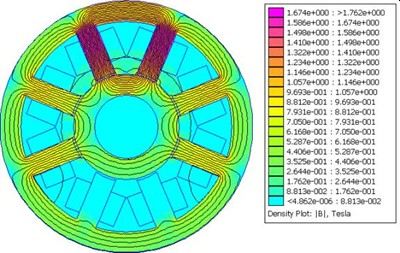
\includegraphics[width=5cm]{pics/es_magnetostatics.jpg}
			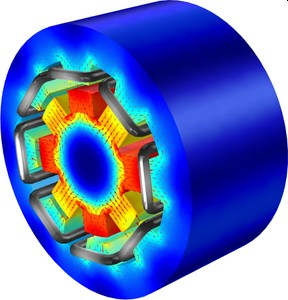
\includegraphics[width=5cm]{pics/es_electrostatics.jpg}
		\caption{Examples of finite element solution to electrostatics/magnetostatics problems (from FEMM and COMSOL documentation)}
		\label{fig:es_electrostatics}
	\end{figure}
	
	
	%\item The \textbf{magnetostatics equation}:
	%\[
	%\mu \nabla^2 \psi = -\xi
	%\]
	%where $\psi(\vect{x})$ is the unknown scalar magnetic potential field in [A] units, 
	%$\mu$ is the permeability [H/m] of the material,
	%$\xi$ is the volume charge density in $\Omega$, divergence of magnetization $\xi = \nabla \cdot \vect{M}$, if any. 
	%\begin{itemize}
		%\item a Dirichlet boundary condition $\phi=\phi_0, \; \forall \vect{x}\in\Gamma_i$ means imposing a magnetic potential [A] on a boundary surface $\Gamma_i$, 
		%\item a Neumann   boundary condition $\partial{\psi}/\partial{\vect{n}}=-H_0 \; \forall \vect{x}\in\Gamma_i$ means imposing a magnetic field intensity [A/m] $H_0$ through a boundary zone $\Gamma_i$, remembering that magnetic field intensity in [A/m] is $\vect{H}=-\nabla \psi$.
	%\end{itemize}
	
	\item The \textbf{Newtonian gravitational field equation}:
	\[
	\nabla^2 \phi = 4 \pi \rho G
	\]
	where $\phi(\vect{x})$ is the unknown scalar gravitational potential field, 
	$\rho$ is the density of the material,
	$G$ is the gravitational constant. 
	\begin{itemize}
		\item a Dirichlet boundary condition $\phi=\phi_0, \; \forall \vect{x}\in\Gamma_i$ means imposing a gravitational potential on a boundary surface $\Gamma_i$, 
		\item a Neumann   boundary condition $\partial{\phi}/\partial{\vect{n}}=g_0 \; \forall \vect{x}\in\Gamma_i$ means imposing a gravitational field $g_0$ perpendicular to a boundary zone $\Gamma_i$, remembering that $\vect{g}= -\nabla \phi$.
	\end{itemize}
	
	
	\item The \textbf{Reynolds equation on lubrication of thin films}:
	\[
	\nabla \cdot (-\vect{q}) =  \rho W
	\]
	where $\vect{q} \in \mathbb{R}^2$ is a mass flow rate 
	$\vect{q}=\rho \left\{ 
	\frac{Uh}{2}-\frac{h^3}{12\eta}\frac{\partial P}{\partial x},
	\frac{Vh}{2}-\frac{h^3}{12\eta}\frac{\partial P}{\partial y}
	\right\}$ 
	that stems from the original Reynolds equation that is often written in  in the more conventional form 
	\[
	 \frac{\partial}{\partial x} \left( \frac{\rho h^3}{12 \eta}\frac{\partial P}{\partial x}\right) 
  +\frac{\partial}{\partial y} \left( \frac{\rho h^3}{12 \eta}\frac{\partial P}{\partial y}\right) 
	= \frac{\partial}{\partial x}\left( \frac{\rho U h}{2}\right)
	+ \frac{\partial}{\partial y}\left( \frac{\rho V h}{2}\right)
	+ \rho W
	\] 
	for $P$ as pressure, $\rho$ as density, $U,V,W$ as (tangential,tangential,vertical) relative surface velocities, $h$ film thickness, $\eta$ viscosity. Boundary conditions often constrain the pressure on the boundary.
	

	\item The Laplace equation is a Poison equation without the source term
	
	\item The thin elastic membrane on rigid support is $K \nabla^2 z = -f$ with $z$ vertical displacement and $f$ is vertical force.
\end{itemize}




\subsection{Diffusion equations}

\textbf{Diffusion equations} are parabolic PDEs of the following type:
\begin{align}
\frac{\partial u}{\partial t}  = \mathbf{\nabla} \cdot (D \mathbf{\nabla} u) + R
\label{eq:diffusion}
\end{align}
where $u$ is the unknown $u(\vect{x},t)$, often scalar-valued but might also be tensor-valued,
$D$ is a diffusivity coefficient, 
$\vect{V}$ is the velocity, 
$R$ is a source (sink) term expressing loads per units of volume.

In the following we list some physical problems that share the same mathematical structure of the diffusion equation, 
all assumed in a 3D domain $\Omega$, with $\vect{x} \in \Omega \subset \mathbb{R}^3$:

\begin{itemize}

	\item The transient \textbf{heat equation}:
	\begin{align}
	\rho c_p \frac{\partial T}{\partial t}   - k\nabla^2 T =  q
	\label{eq:transientheat}
	\end{align}
	where $T(\vect{x})$ is the unknown temperature field in [K] units, 
	$\rho$ is the material density [kg/m${}^3$], 
	$c_p$ is the material specific heat capacity [J/(K kg)], 
	$k$ is the thermal conductivity [W/(m K)], 
	$q$ is the heat-flux [W/m${}^3$] of sources in $\Omega$ if any - for example heat from uranium fission. 
	Note that with no $q$ source, and by introducing the thermal diffusivity $\alpha=k/(\rho c_p)$, in [m${}^2$/s], one has the more conventional heat equation $\frac{\partial T}{\partial t} - \alpha \nabla^2 T=0$, and here one recognize that $\alpha$ is the $D$ is a diffusivity coefficient in \eqref{eq:diffusion}.
	Also note that assuming steady state, $\frac{\partial T}{\partial t} = 0$, hence the Poisson equation for steady state heat $k\nabla^2 T = -q$ is a special case of this.
	Boundary and initial conditions:
	\begin{itemize}
		\item a Dirichlet boundary condition $T=T_i, \; \forall \vect{x}\in\Gamma_i$ means imposing a temperature on a boundary surface $\Gamma_i$, 
		\item a Neumann   boundary condition $-k\partial{T}/\partial{\vect{n}}=q_0 \; \forall \vect{x}\in\Gamma_i$ means imposing a heat flux $q_0$ [W/m${}^2$] through a boundary zone $\Gamma_i$, remembering $\vect{q}=-k \nabla T$.
		\item a initial condition $T=T_0$ at time $t=0$.
	\end{itemize}
	
	\item the \textbf{second Fick equation}, governing the transport of mass through diffusive means (dilution in liquids, gases, asdorption in porous media, etc.)
	\[
	\frac{\partial \phi}{\partial t}   - D \nabla^2 \phi =  0
	\]
	where $\phi(\vect{x})$ is the unknown concentration of a substance (ex. in [mol/m${}^3$]), $D$ is the diffusion coefficient, in [m${}^2$/s].
	
\end{itemize}







\subsection{Convection-diffusion equations}

\textbf{Convection-diffusion equations}, sometimes advection-diffusion depending on the context, are PDEs of the following type:
\begin{align}
\frac{\partial u}{\partial t}  = \mathbf{\nabla} \cdot (D \mathbf{\nabla} u) - \mathbf{\nabla} \cdot (\vect{v} u) + R
\end{align}
where $u$ is the unknown $u(\vect{x},t)$, often scalar-valued but might also be tensor-valued,
$D$ is a diffusivity coefficient, 
$\vect{v}$ is the velocity, 
$R$ is a source (sink) term expressing loads per units of volume.

In the following we list some physical problems that share the same mathematical structure of the diffusion equation, 
all assumed in a 3D domain $\Omega$, with $\vect{x} \in \Omega \subset \mathbb{R}^3$:

\begin{itemize}

\item the \textbf{Smoluchowski equation} of drift-diffusion equation, 
\[
\frac{\partial \phi}{\partial t}  = \nabla \cdot (D \nabla \phi) - \nabla \cdot \left( \zeta^{-1} \vect{F} \phi \right) + R
\]
similar to the second Fick equation governing the transport of mass through diffusive means (dilution in liquids, gases, asdorption in porous media, etc.) but also adding a force field $\vect{F}$ as in electrophoresis and assuming a viscous drag so that velocity is $\vect{v}=\zeta^{-1} \vect{F}$. Again, $\phi(\vect{x})$ is the unknown concentration of a substance (ex. in [mol/m${}^3$]), $D$ is the diffusion coefficient, in [m${}^2$/s]. 
This is also similar to the \textbf{Fokker-Plank equation} if one considers the probability density function of velocities of particles in brownian motion instead of concentrations.

\item the incompressible Navier-Stokes equation is closely related to a convection-diffusion problem as:
\[
\frac{\partial \vect{M}}{\partial t} = \frac{\mu}{\rho} \nabla^2 \vect{M} -\vect{v} \cdot \nabla \vect{M} + (\vect{f}-\nabla P)
\]
where $\vect{M} = \rho \vect{v}$ is fluid momentum per unit of volume, $\mu$ is viscosity, $P$ is pressure, $\vect{f}$ is a load per unit of volume, for instance gravity.

\end{itemize}






\subsection{Linear elasticity equations}

\begin{figure}
		\centering
			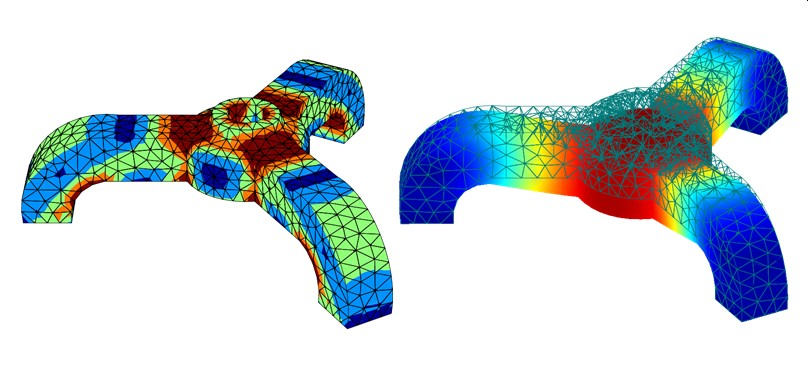
\includegraphics[width=12cm]{pics/es_elasticity.jpg}
		\caption{Example of finite element solution to a linear elasticity problem (from GETFem++ documentation)}
		\label{fig:es_elasticity}
	\end{figure}
	
	
A basic representation of \textbf{linear elasticity} is given by the following PDE, embedding an equilibrium equation, a strain-displacement equation, and a constitutive equation: 
\begin{align}
	\left\{
	\begin{aligned}
		 & \nabla \cdot \tensor{\sigma} + \tensor{b} = \vect{0} \\
		 & \tensor{\epsilon} = \frac{1}{2} \left( \nabla \vect{u} + \nabla \vect{u}^T \right) \\
		 & \tensor{\sigma} = \tensor{C} : \tensor{\epsilon}
	\end{aligned}
	\right.
\end{align}
where 
$\vect{u}$ is the unknown vector displacement field,
$\vect{b}$ is an applied per-unit-of-volume load,
$\tensor{\epsilon}$ is the strain rank-2 tensor,
$\tensor{\sigma}$ is the stress rank-2 tensor,
$\tensor{C}$ is the stiffness rank-4 tensor. %, of whose $3^4=81$ components only two are independent in a isotropic material, ex. Poisson ratio and Young modulus.

For isotropic elasticity, where $\tensor{C}$ can be made dependant on just two parameters and 
$\tensor{\sigma}=2\mu \tensor{\epsilon} +\lambda \; \mathrm{tr}(\tensor{\epsilon})\tensor{I}$,
one can also write the more compact expression as \textbf{Navier-Lamé equation}:
\[
\mu \nabla^2 \vect{u} + (\lambda + \mu) \nabla ( \nabla \cdot \vect{u}) + \tensor{b} = \vect{0}
\]
with the Lamé constants 
$\lambda = \frac{E\nu}{(1+\nu)(1-2\nu)}$ and 
$\mu = G = \frac{E}{2(1+\nu)}$.
This is again a PDE. 

\begin{itemize}
		\item a Dirichlet boundary condition $\vect{u}=\vect{u}_0, \; \forall \vect{x}\in\Gamma_i$ means imposing a known displacement (hence a known position) on a boundary surface $\Gamma_i$, 
		\item a Neumann boundary condition $\tensor{\sigma} \cdot \vect{n} = \vect{t}_0 \; \forall \vect{x}\in\Gamma_i$ means imposing a known traction $\vect{t}_0$ on the boundary surface $\Gamma_i$.
	\end{itemize}




\subsection{Navier-Stokes equations}

The \textbf{compressible Navier-Stokes equation} describes the motion of fluids under very general assumptions:
\begin{align}
		 \rho \frac{\partial \vect{v}}{\partial t} + \rho \,\vect{v} \cdot \nabla \vect{v} - \mu \, \nabla^2 \vect{v} + \nabla \bar{p}  - \tfrac13 \mu \, \nabla (\nabla\cdot\vect{v}) - \vect{f} = \vect{0}
\label{eq:navierstokes}
\end{align}
It stems from the following assumptions:
\begin{itemize}
	\item the Cauchy momentum equation $\rho \frac{D\vect{v}}{Dt} = \nabla \cdot \tensor{\sigma} + \vect{f}$, with material derivative $D\vect{v}/Dt = \partial \vect{v}/\partial t + \rho \vect{v} \cdot \nabla \vect{v}$,
	\item the rate of strain is $\tensor{\epsilon}=\frac{1}{2}(\nabla\vect{v}+\nabla{\vect{v}}^T)$,
	\item the linear stress constitutive equation is a isotropic function of rate of strain as 
	$\tensor{\sigma} = \zeta (\nabla\cdot\vect{v}) \mathbf I + \mu \left(\nabla\vect{v} + ( \nabla\vect{v} )^{T} - \tfrac23 (\nabla\cdot\vect{v}) \tensor{I}\right)$ 
	\item the continuity equation for balance of mass: $\frac{\partial \rho}{\partial t} = \nabla \cdot (\rho\vect{v})$
\end{itemize}
where $\vect{v}$ is velocity, $\mu$ is dynamic viscosity, $\lambda$ is bulk viscosity, $\zeta$ is the "dilational" second viscosity as in $\zeta \equiv \lambda + \tfrac23 \mu$, pressure is $\bar{p}= p - \zeta \lambda \cdot \vect{v}$, external loads per unit of volume are $\vect{f}$, in many cases $\vect{f}=\rho\vect{g}$ where $\vect{g}$ is gravity acceleration field.

\begin{itemize}

\item The \textbf{incompressible Navier-Stokes equation} is a special case of the Navier-Stokes equations. Except for particular problems at high Mach numbers, in fact, the compressibility of the fluid can be neglected. Again with the assumption of isotropic Newtonian fluids, and recovering the continuity condition as $\nabla\cdot\vect{v}=0$
\begin{align}
	\left\{
	\begin{aligned}
		  \rho\frac{\partial\vect{v}}{dt} + \rho \,\vect{v} \cdot \nabla \vect{v} - \mu \,\nabla^2 \vect{v}  +\boldsymbol{\nabla}p - \vect{f} &= \vect{0} \\
			\nabla\cdot\vect{v}&= 0
	\end{aligned}
	\right.
	\label{eq:stokes}
\end{align}


\item The \textbf{steady state Navier-Stokes equation} is a special case of the Navier-Stokes equations with no dependence on time. 
With the simplification of Newtonian fluid and incompressible flow one has:
\begin{align}
	\left\{
	\begin{aligned}
		  \rho \,\vect{v} \cdot \nabla \vect{v} - \mu \,\nabla^2 \vect{v}  +\boldsymbol{\nabla}p - \vect{f} &= \vect{0} \\
			\nabla\cdot\vect{v}&= 0
	\end{aligned}
	\right.
	\label{eq:stokes}
\end{align}


\item The \textbf{Stokes equations} is a special case of the steady state Navier-Stokes equations where the advective terms are negligible respect to the viscous forces, as in slow creeping fluids with low Reynolds numbers $Re \rightarrow 0$. With simplification of Newtonian fluid and incompressible flow one has:
\begin{align}
	\left\{
	\begin{aligned}
		  -\mu \,\nabla^2 \vect{v} +\boldsymbol{\nabla}p - \vect{f} &= \vect{0} \\
			\nabla\cdot\vect{v}&= 0
	\end{aligned}
	\right.
	\label{eq:stokes}
\end{align}

\item The \textbf{inviscid Euler equations} is a special case of the Navier-Stokes equations where the diffusive terms are negligible, as in high Reynolds numbers $Re \rightarrow \infty$. With simplification of Newtonian fluid and incompressible flow one has:
\begin{align}
	\left\{
	\begin{aligned}
		  \rho\frac{\partial\vect{v}}{dt} + \rho \vect{v} \cdot \nabla \vect{v} + \boldsymbol{\nabla}p - \vect{f} &= \vect{0} \\
			\nabla\cdot\vect{v}&= 0
	\end{aligned}
	\right.
	\label{eq:stokes}
\end{align}


\end{itemize}


\begin{figure}
		\centering
			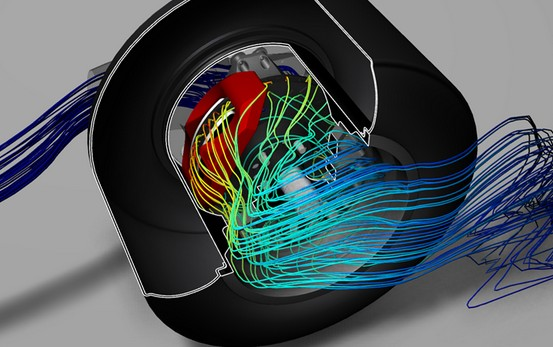
\includegraphics[height=4cm]{pics/es_cfd.jpg}
			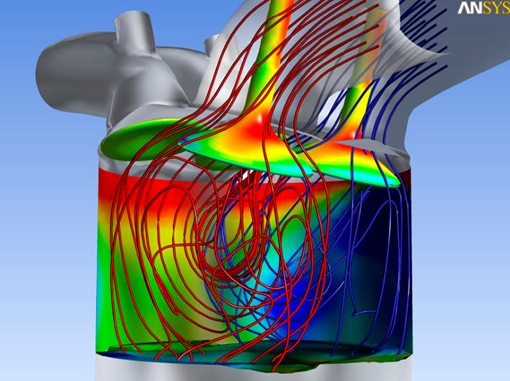
\includegraphics[height=4cm]{pics/es_cfd2.jpg}
		\caption{Examples of computational fluid dynamics, left: with finite elements (Autodesk CFD simulator), right: with finite volume method (from ANSYS Fluent documentation)}
		\label{fig:es_cfd}
	\end{figure}


\subsection{Exercises}

{
\small

\begin{enumerate}
	
	\item Write the strong form of the straight Euler-Bernoulli beam theory in linear elasticity. Extend it to the case of dynamics, adding inertial forces caused by a linear mass density of the beam.
	
	\item Write the strong form of the straight Timoshenko beam theory, where shear is taken into account. Extend it to the case of dynamics, adding inertial forces.
	
	\item Write the strong form of the geometrically-exact beam theory (Cosserat rods).  Extend it to the case of dynamics, adding inertial forces.
	
	\item Write the strong form of the Kirchhoff-Love plate, where one assumes that segments normal to the mid-surface remain straight and normal to the mid-surface after deformation. Add the contribution of inertial forces. 
	Write the strain-displacement relations to compute $\epsilon_{\alpha\beta}$ from the normal displacement field $u$, where $\alpha$ and $\beta$ can be either direction 1 or 2 of the plate, and show that $\epsilon_{\alpha 3}$ and $\epsilon_{33}$ are always null.
	
	\item Write the strong form of the Reissner-Mindlin plate, that extends the Kirchhoff-Love plate theory by taking into account also the effect of shear. Add the contribution of inertial forces.
	
\end{enumerate}

}





\newpage
\section{Discretization}

There are different ways to cast the previous infinite dimensional problems into finite dimensional problems that can be attacked with computational tools. Among the different strategies we mention the finite element method, the finite different method, the finite volume method, etc. In the following we will focus on the finite element Galerkin method.

Deeper insights on the finite element method can be found in the books of the authors that pioneered it, such as \cite{zienkiewiczFEA1977,tjrhughes87,bathe1982,wriggers2006} to name a few.


\subsection{Function spaces}

The following is a primer on basic concepts of functional analysis, this is useful because literature on FEA often cite concepts like Sobolev spaces etc.

\begin{itemize}
	\item A \textbf{vector space}, over a scalar field $K \in \mathbb{R}$, is a set $V$ equipped with 
	addition $+: V \times V \rightarrow V$, commutative and associative, 
	and scalar multiplication $\cdot: F \times V \rightarrow V$, distributive and associative.
	
	\item An \textbf{inner product space} is a vector space equipped with an inner product, $\left\langle\cdot,\cdot\right\rangle : V \times V \rightarrow F$.
	
	\item A \textbf{normed vector space} is a vector space equipped with a norm, $\| \cdot \| : V \rightarrow \mathbb{R}$.
	
	\item A $L^p$-norm is a norm defined as $\| \vect{x} \|_p = \left( |x_1|^p + |x_2|^p + \dotsb + |x_n|^p \right) ^{1/p}$, the Euclidean $L^2$ norm being the most common.
	
	\item A space $V$ is \textbf{complete} if all Cauchy sequences converge to an element in $V$.
	
	\item A \textbf{Banach} space is a complete normed vector space.
	
	\item A \textbf{Hilbert}\footnote{It is remarkable how many bright scientists attended the University of Göttingen.} space is a complete normed inner product space.
	
	\item A \textbf{function space} is a topological space whose points are functions. Some examples will follow.
	
	
	
	\begin{itemize}
		\item $B$ is the space of \textit{bounded} functions
		
		\item $C$ is the space of \textit{continuous} functions
		
		\item $C_c$ is the space of \textit{continuous} functions with compact support
		
		\item $C^r$ is the space of functions that are \textit{continuous} up to the first $r$ \textit{derivatives}
		
		\item $C^\infty$ is the space of \textit{smooth functions}, ex. $f=\sin(x)$.
		
		\item $L^p$ is the \textbf{Lebesgue space} of measurable functions with finite norm $\| f \|_{L^p}=\left( \int_\Omega |f|^p d\mu \right)^{1/p}$, these functions are not necessarily continuous.
		\[
		L^p(\Omega) = \left\{ f \; \left| \; \int_\Omega |f|^p d\mu < \infty \right. \right\}
		\]
		
		\item Lebesgue $L^p$ space is a Banach space with norm 
		$\| f \|_{L^p}=\left( \int_\Omega |f|^p d\mu \right)^{1/p}$.
		
		\item Lebesgue $L^2$ space is a Hilbert space with inner product 
		$\left\langle u , v \right\rangle_{L^2} = \int_\Omega u v d\mu$.
		
		\item Let $f \in L^2(\Omega)$, the \textit{weak derivative} $\partial^\alpha f$ of order $\alpha$ is a function in $L^2(\Omega)$ that satisfies:
		\[
		\int_\Omega \partial^\alpha f \psi d\mu =  (-1)^{|\alpha|} \int_\Omega f \partial^{|\alpha|} \psi d\mu, \quad \forall \psi 
		\in C^{\infty}_c
		\]
		It does not require the function to be differentiable, it is enough that it is integrable.
		
		\item  $W^{m,p}$ is the \textbf{Sobolev space} is the subspace of $L^p(\Omega)$ functions which possess up to order-$m$ weak derivatives $\partial^\alpha$, with $\alpha \leq m$.
		\[
		W^{m,p}(\Omega) = \left\{ f \in L^p(\Omega) \; | \; \partial^\alpha f \in L^p(\Omega), 1\leq  \alpha \leq m \right\}
		\]
		
		\item  $H^m$ is the \textbf{Hilbert-Sobolev space} more in detail is a $W^{m,2}$ space:
		\[
		H^m(\Omega) = \left\{ f \in L^2(\Omega) \; | \; \partial^\alpha f \in L^2(\Omega), 1\leq  \alpha \leq m \right\}
		\]
		
		\item The norm in $H^m$ is defined as
		\[
		\| f \|_{H^m} = \left( \sum_{\alpha=0}^m \int_\Omega |\partial^\alpha f|^2 d\mu \right)^{1/2} \; = \; 
							    \left( \sum_{\alpha=0}^m \int_\Omega ||\partial^\alpha f||^2_{L^2} d\mu \right)^{1/2}
		\]
		

		\item The importance of Sobolev space is that solutions of PDEs are often searched in $H^m$ space (so called \textit{weak}, or integral solutions) rather than in the $C^k$ space (as in \textit{strong} solutions for order-k PDEs), thus relaxing the continuity requirement.
		
		\item We denote with $H^m_0$ the subspace of $H^m$ with $m-1$ derivatives equal to zero at the boundary.
		
		\item In detail $H^1_0$ is the subspace of $H^1$ functions that are zero at the boundary. 
		
		\item In detail $H^1_g$ is the subspace of $H^1$ functions that have a prescribed value $g$ at the boundary.
		
		\item Functions in $H^m$ are required to be in $C^{m-1}$.
		
		\item Example: the step function is in $L^2$ but not in $H^1$ (as derivative contains Dirac deltas), the hat function is in $L^2$ and in $H^1$, meanwhile it is in $C^0$. 
		
	\end{itemize}
	
\end{itemize}

\subsection{The weak formulation}

The weak formulation reduces the regularity assumptions for the solution of the PDE: whereas the solution of the original PDE must be in $C^2$, the weak solution must be only in $H^1_0$, a requirement that makes the problem much more practical. This is the positive side effect of using an integral (variational) form of the equations. 

We introduce the weak formulation starting from the case of a generic Poisson equation (a PDE like the steady state heat equation or the electrostatic problem already discussed previously) with unknown scalar function $u$, paired with Dirichlet and Neumann boundary conditions:

\begin{align}
\boxed{
	\left\{
	\begin{aligned}
			& k\nabla^2 u + f = 0	& \forall \vect{x}\in\Omega \\ 
			& u=u_D, \; 					& \forall \vect{x}\in\Gamma_D \\
			& k\partial{u}/\partial{\vect{n}}=q_N \; & \forall \vect{x}\in\Gamma_N
	\end{aligned}
	\right.
	\label{eq:strongpoisson}
	}
\end{align}

A solution to the strong form above should satisfy $u \in C^2(\Omega)$, that is, at least it should be twice differentiable over the entire domain $\Omega$. 

We will rewrite it as a weak formulation, that requires less stringent requirement on the functional class of the solution -letting it to be approximated by a piecewise polynomial $u^h \approx u$ at the end. In fact we will assume a $u \in H^1_{u_D}(\Omega)$, that is we assume the solution to be a function with just the first derivative being square integrable, and with prescribed value $u_D$ at the boundary in order to satisfy the Dirichlet boundary condition.

We also introduce a \textit{test function}, namely $v \in H^1_0(\Omega)$, assumed null at the $\Gamma_D$ boundary. 
For compactness we introduce functional spaces $\mathcal{U}$ and $\mathcal{U}_0$ as:
\begin{align}
	u \in \mathcal{U}   &=& \left\{  u \in H^1(\Omega) \; : \; u=u_D \forall \vect{x} \in \Gamma_D \right\} \\
	v \in \mathcal{U}_0 &=& \left\{  v \in H^1(\Omega) \; : \; v=0   \forall \vect{x} \in \Gamma_D \right\}
\end{align}



We start multiplying the terms of the PDE by the test function $v$ and we integrate over the domain, obtaining:
\begin{align}
	\int_\Omega v \, k\nabla^2 u  \, d\Omega + \int_\Omega  v \, f \, d\Omega = 0
	\label{eq:weakpoisson01}
\end{align}

The first term can be integrated by parts (or just applying the Leibnitz product rule, that leads here to the known property of divergence operator: $\nabla\cdot\left(v\mathbf{A}\right)= v\nabla\cdot\mathbf{A}+\mathbf{A}\cdot\nabla v$ where our $\nabla^2 u$ is in fact $\nabla\cdot\mathbf{A}$ for $\mathbf{A}=\nabla u$) thus obtaining:
\begin{align}
	\int_\Omega k \nabla \cdot (v \nabla u)  \,d\Omega - \int_\Omega k \nabla v \cdot \nabla u \,d\Omega    + \int_\Omega  v \, f  \,d\Omega = 0
	\label{eq:weakpoisson02}
\end{align}

Then, we use the Gauss divergence theorem to turn the first term into a boundary integral:
\[
\int_\Omega k \nabla \cdot (v \nabla u)  \,d\Omega = \int_{\Gamma} k v \nabla u \cdot \vect{n} \,d\Gamma
\]
where on the Dirichlet boundaries $\Gamma_D$ it simplifies to zero because $v=0$ on $\Gamma_D$ by construction, whereas on the 
boundaries $\Gamma_N$ it assumes the value prescribed by Neumann condition as $ k \partial{u}/\partial{\vect{n}} = k \nabla u \cdot \vect{n} = q_N$:
\begin{align}
\int_{\Gamma_D} k v \nabla u \cdot \vect{n} \,d\Gamma_D &= 0 \\
\int_{\Gamma_N} k v \nabla u \cdot \vect{n} \,d\Gamma_N &= \int_{\Gamma_N} v \, q_N \,d\Gamma_N
\end{align}

Substitute the above in \eqref{eq:weakpoisson02} and see that the weak formulation simplifies to:
\begin{align}
  \int_\Omega k \nabla v \cdot \nabla u \,d\Omega = \int_\Omega  v \, f  \,d\Omega  + \int_{\Gamma_N} v \, q_N \,d\Gamma_N
	\label{eq:weakpoisson}
\end{align}

We note in passing that going to the weak formulation of the Poisson equation, the original $\nabla^2$ term disappeared, 
and now it does not require anything more than the first derivative of $u$ to be integrable 
(and same for the test function $v$).

Also note that if no Neumann conditions are required it, the weak formulation simplifies even more: 
\[
\int_\Omega k \nabla v \cdot \nabla u \,d\Omega = \int_\Omega  v \, f \,d\Omega 
\]

The weak formulation \eqref{eq:weakpoisson} can be rewritten with a more compact notation, introducing a
bilinear operator 
$\mathcal{B}: \mathcal{U} \times \mathcal{U}_0 \rightarrow \mathbb{R}$ 
and a linear operator 
$\mathcal{L}:  \mathcal{U}_0 \rightarrow \mathbb{R}$ 
that, in our Poisson case above, are:
\begin{align}
  \mathcal{B}(u,v) &= \int_\Omega k \nabla v \cdot \nabla u \,d\Omega      \label{eq:bilinearop}\\
	\mathcal{L}(v)   &= \int_\Omega v \, f \,d\Omega    + \int_{\Gamma_N} v \, q_N \,d\Gamma_N         \label{eq:linearop}
\end{align}

This said, the weak form can be written as
\begin{align}
\boxed{
\mathcal{B}(u,v) = \mathcal{L}(v)
}
\label{eq:weakbl}
\end{align}
In the following we see that most of the PDE problems seen in the previous sections can be expressed with a sum of bilinear and linear terms like the above (but the expressions of the bilinear and linear operators can be different in the sense that the integrands could have different expressions).

We remark in passing that, for symmetrical $\mathcal{B}(u,v)$, \eqref{eq:weakbl} is equivalent to a variational problem $u = \mathrm{argmin}_{u}I[u]$ with the functional $I[u]=\frac{1}{2}\mathcal{B}(u,u) - \mathcal{L}(u)$ representing some form of energy, and whose stationary condition is $\mathcal{B}(u,\partial u) - \mathcal{L}(\partial u) = 0$; note how in elasticity the $\partial u$ can be considered a virtual displacement, and this turns into the principle of virtual work. 



\subsection{Discretization}

Now, one can introduce an approximation of $u$ and $v$, to pass from an infinite-dimensional problem to a finite-dimensional problem that depends on a countable set of variables, hence more computer-friendly. 
We assume a discretized approximate solution $u^h \approx u$, with $u^h \in \mathcal{U}^h \subset \mathcal{U}$. 
Here $h$ represents the discretization size, and $u^h \rightarrow u$ as $h\downarrow 0$.
Similarly, $v^h \approx v$, with $v^h \in \mathcal{U}_0^h \subset \mathcal{U}_0$. 

The finite-dimensional function spaces $\mathcal{U}^h, \mathcal{U}_0^h$ are built using $n$ \textit{shape functions}, here named $N_i(\vect{x})$, as in:
\begin{align}
u^h(\vect{x}) &= \sum_i^n \hat{u}_i N_i(\vect{x}) \\
v^h(\vect{x}) &= \sum_j^n \hat{v}_j N_j(\vect{x})
\end{align}

Thank to this discretization, the unknown is not a function $u$ anymore, but it is rather a vector with a finite amount of $\hat{u}_i$ unknowns. 
We also remark that one can split the entire domain $\Omega$ in multiple finite elements, each with its $\hat{u}_i$ unknowns, leading to a finer 
discretization and to a larger amount of $\hat{u}_i$ unknowns. 

Shape functions can be linear, quadratic, etc., depending on the finite element type.

This variational setting is attributed to W.Ritz\footnote{It is remarkable how many bright scientists attended the University of Göttingen.}
and B.Gal{\"e}rkin\footnote{The pronounciation of {\"e} in russian sounds like \textit{yo}, so one should pronounce \textit{Galyorkin}, I do not why everyone spells it Gal\textit{e}rkin.}, hence the name \textbf{Galerkin} method. More in detail, if the same approximation space is used for both $u$ and $v$, this is sometimes referred as \textbf{Bubnov-Galerkin} method, and if a different approximation space is chosen for $v$, this is called \textbf{Petrov-Galerkin} method. 
The modern mathematical setting and terminology for the finite element method is credited to R.Courant\footnote{It is remarkable how many bright scientists attended the University of Göttingen.}.

Using the discretization, the weak form can be written:
\begin{align}
\mathcal{B}(u^h,v^h) &= \mathcal{L}(v^h) \\
\mathcal{B}\left(\sum_i^n u_i N_i(\vect{x}),\sum_j^n v_j N_j(\vect{x})\right) &= \mathcal{L}\left(\sum_j^n v_j N_j(\vect{x})\right)
\end{align}

Exploiting the fact that $\mathcal{B}$ is bilinear and $\mathcal{L}$ is linear, one can take the $\hat{u}_i$ and $\hat{v}_i$ weights outside integrals, leading to:
\begin{align}
\sum_j^n \hat{v}_j \sum_i^n \hat{u}_i \mathcal{B}\left(N_i(\vect{x}),N_j(\vect{x})\right) &= \sum_j^n \hat{v}_j \mathcal{L}\left( N_j(\vect{x})\right)
\end{align}

One can simplify the $\hat{v}_j$ terms and obtain a very simple form of the discretized weak form where one can see that the bilinear and linear operators act only on the shape functions:
\begin{align}
\sum_i^n \hat{u}_i \mathcal{B}\left(N_i(\vect{x}),N_j(\vect{x})\right) &= \mathcal{L}\left( N_j(\vect{x})\right)
\end{align}

In sake of further compactness one can group all $\hat{u}_i$ in the vector of unknowns $\hat{\vect{u}}$, introduce a matrix $\matr{K} \in \mathbb{R}^{n\times n}$ and a vector $\vect{b} \in \mathbb{R}^{n}$, and obtain a linear system: 
\begin{align}
\boxed{
\begin{aligned}
\matr{K} \hat{\vect{u}}  &= \vect{b} & \\[2mm]
 K_{ij}   &=  \mathcal{B}\left(N_i,N_j \right) \\
 b_j &=  \mathcal{L}\left( N_j )\right)
\end{aligned}
}
\end{align}
This $\matr{K} \vect{u} = \vect{b}$ linear system gives the solution $\vect{u}$ to the discretized PDE problem. Of course, the finer the discretization, the larger the size of $\hat{\vect{u}}$, hence the larger the matrix $\matr{K}$, and the more computationally intensive is the solution. To this end, one might consider using special types of solvers, such as Krylov solvers, that exploit the fact that in many cases the $\matr{K}$ matrix is sparse and contains many structural zeros: please go to the section on linear solvers for a primer on this topic. 


\subsection{Quadrature}

One can see that, for computing the elements of $\matr{K}$, in our example of the Poisson equation, one needs to compute 
\[
K_{ij}  = \mathcal{B}\left(N_i,N_j \right) = \int_\Omega k \nabla N_i(\vect{x}) \cdot \nabla N_j(\vect{x}) d\Omega
\]
just like for the elements of $\vect{b}$ one computes
\[
b_j  = \mathcal{L}\left( N_j )\right) = \int_\Omega N_i(\vect{x}) \, f \,d\Omega + \int_{\Gamma_N} N_i(\vect{x}) \, q_N \,d\Gamma_N
\]
This amounts to performing some type of integration over a domain (the finite element volume, for instance) per each term. This can be
done via analytical methods only in limited cases, otherwise using Newton-Cotes quadrature, or Gauss-Legendre quadrature, or other approximations. 
We discuss the Gauss quadrature briefly, ie. an approximation of the integral via a weighted sum of values sampled in some Gauss points $\vect{x}_g$ scattered in the volume domain.

In general, Gauss integration over $n{GP}$ Gauss points with corresponding $w_g$ weights at $\vect{x}_g$ abscyssae points is done with a sum, for example:
\begin{align*}
\int_\Omega k \nabla N_i(\vect{x}) \cdot \nabla N_j(\vect{x}) d\Omega &= \sum_{g=1..n_{GP}} w_g \nabla N_i(\vect{x}_g) \cdot \nabla N_j(\vect{x}_g)
\end{align*}
and the same for other bilinear/linear terms.
 
The lower the degree of shape functions, the smaller the amount of Gauss point samples that are needed to correctly compute the quadrature; for example, a tetrahedral finite element with its four linear shape functions requires only a single Gauss point in the middle, etc. 

Note, however, that most often the $w_g$ and values are tabulated assuming generic abscyssae $\zeta_g$ ranging in the $[-1,+1]$ interval, hence one has to express $\vect{x}=\vect{x}(\vect{\zeta})$ (as happens in the \textit{isoparametric} finite element approach, where $\vect{\zeta}$ for example contains the three parametric coordinates along the direction of a brick each ranging in $[-1,+1]$ and shape functions are functions of these parametric coordinates) and simply scale the result using jacobians $\partial\vect{x}/\partial\vect{\zeta}$ as in
\[
\int_a^b f(x) dx = \int_{-1}^{+1} J_{\zeta} f(\zeta) d\zeta \approx J_{\zeta} \sum_{g=1..n_{GP}} w_g f(\zeta_g)
\]
that in our case would lead to:
\begin{align*}
\int_\Omega k \nabla N_i(\vect{x}) \cdot \nabla N_j(\vect{x}) d\Omega \approx J_{\vect{\zeta}} \sum_{g=1..n_{GP}} w_g \nabla N_i(\vect{\zeta}_g) \cdot \nabla N_j(\vect{\zeta}_g)
\end{align*} 

The reader interested in quadrature should look also at the following connected problems: \textit{hourglass modes} (zero-energy spurious modes), selective and \textit{reduced integration}, \textit{shear locking} (ex.in Timoshenko beams) and how to get rid of it using ad-hoc integration.


\subsection{Constraints}

Apart from the already mentioned treatment of Dirichlet and Neumann conditions, a straightforward and powerful way to apply generic constraints to nodes of a FE mesh -especially in a context of mechanical problems where nodes represent points of a deformable material- is to couple the discretized PDE with algebraic constraints. A (possibly linear) constraint equation is a function that gives zero residual when satisfied:
\[
\vect{C}(\hat{\vect{u}})=\vect{0}
\]
For example, in the context of 3D continuum elasticity, if one requires that the displacement $\hat{\vect{u}}_k$ of the $k$-th node is equal to some $\overline{\vect{u}}$ value, one would write:
\[
\vect{C}(\hat{\vect{u}}) = \hat{\vect{u}}_k - \overline{\vect{u}} 
\]
Another example, again with a node in a 3D continuum: if one requires the node to be able to move on the yz plane of a coordinate system with rotation matrix $\matr{R}$, while precluding the x displacement relative to such coordinate system, one would write:
\[
\vect{C}(\hat{\vect{u}}) = [1, 0, 0] \matr{R}^T \hat{\vect{u}}_k  
\]

One can add multiple constraints in this way, obtaining a large $\vect{C}(\hat{\vect{u}})$ vector of $m$ scalar constraints, $\vect{C}:\mathbb{R}^n \rightarrow \mathbb{R}^m$. 
The constraint jacobian is a matrix $\matr{C}_u \in \mathbb{R}^{m \times n}$:
\[
\matr{C}_u = \frac{\partial \vect{C}(\hat{\vect{u}})}{\partial \hat{\vect{u}}}
\]
Not all $m$ constraints act on all the $n$ variables of the system-wide $\hat{\vect{u}}$ vector, so the jacobian is often a very sparse matrix.

By linearizing the constraint equation, one has
\[
\vect{C}(\hat{\vect{u}}) \approx \matr{C}_u (\hat{\vect{u}}-\hat{\vect{u}}_0) + \vect{C}(\hat{\vect{u}}_0)
\]
where here we pose $\hat{\vect{u}}_0 = \vect{0}$, thus the constraint equations leads to a linear algebra equation 
$\matr{C}_u \hat{\vect{u}} + \vect{C}(\hat{\vect{u}}_0) = \vect{0}$.

Roughly speaking, the transpose of the jacobian matrix multiplied by a unknown multiplier $\vect{\lambda}$ gives a reaction force in global coordinates, where the unknown multiplier is the reaction in the coordinates of the constraint, therefore the final linear system to be solved becomes:

\begin{align}
\boxed{
\begin{bmatrix}
	\matr{K} & \matr{C}_u^T \\
	\matr{C}_u  & \matr{0}
\end{bmatrix}
\begin{Bmatrix}
	\hat{\vect{u}} \\
	\vect{\lambda}
\end{Bmatrix}
=
\begin{Bmatrix}
	\vect{b} \\
	-\vect{C}(\vect{u}_0)
\end{Bmatrix}
}
\end{align}

The structure of the linear system above, featuring a square matrix $\matr{K}$ bordered to the right and below by constraint jacobians $\matr{C}_u$ and additional unknown multipliers $\vect{\lambda}$ (the constraint reaction forces in this case) like in a Karush Kuhn Tucker (KKT) matrix, is very frequent in other problems involving constraints - not only in structural mechanics. Solving the KKT matrices efficiently is a key to a robust and fast computational tool.

The question is: we added constraints using the KKT matrix by enforcing constraints at level of an already discretized problem, but is it possible to recover the same KKT machinery also if the constraints are defined in the previous step, i.e. when the formulation is still infinite-dimensional? The answer is yes, but the variational procedure is left to the user.


\subsection{Weak formulations for other classes of problems}

So far, we have seen how to translate a Poisson problem (stationary heat problem, magnetostatics, Reynolds lubrication etc.) into a corresponding weak form, and from the weak form we obtained a discretized problem to be solved via a linear system. One can see that other weak formulations can be derived for other classes of problems. For sake of compactness here we present just a few.

\begin{itemize}
	\item Weak form of the Navier-Lamé (linar elasticity) equation:
	\begin{align}
	\int_\Omega \tensor{\sigma}(\vect{u}) : \tensor{\epsilon}(\vect{v}) \,d\Omega = 
	 \int_\Omega \vect{f} \cdot \vect{v} \,d\Omega + 
	 \int_\Gamma \tensor{\sigma}(\vect{u}) \vect{n} \cdot \vect{v} \,d\Gamma   
	\end{align}
	This can be again expressed as $\mathcal{B}(\vect{u}^h,\vect{v}^h) = \mathcal{L}(\vect{v}^h)$, and therefore also to a linear system 
	\[
	\matr{K}\hat{\vect{u}}=\vect{b}
	\]
	once discretized (but look how the expression of $\mathcal{B}$ changes respect to the Poisson problem).
	
	
	\item Weak form of the steady-state incompressible Navier-Stokes equation:
	\begin{align}
	\left\{
	\begin{aligned}
   \int_{\Omega} \mu \nabla \boldsymbol u \cdot \nabla \boldsymbol v  + \int_{\Omega}\rho (\boldsymbol u \cdot \nabla) \boldsymbol u \cdot \boldsymbol v  
	- \int_{\Omega} p \nabla \cdot \boldsymbol v &= \int_{\Omega}\boldsymbol f \cdot \boldsymbol v +  \int_{\Gamma_N} \boldsymbol h \cdot \boldsymbol v\\
	\int_{\Omega} q \nabla \cdot \boldsymbol u &= 0 
	\end{aligned}
	\right.
	\end{align}
	assuming a Dirichlet condition $\tensor{\sigma}(\boldsymbol u, p) \boldsymbol{n} = \boldsymbol h$ in $\Gamma_N$.
	Note that this required an additional test function $q$, for the incompressibility constraint, and note that the discretization will lead to a KKT matrix, 
	%
\begin{align*}
\begin{bmatrix}
	\matr{K} & \matr{C}_u^T \\
	\matr{C}_u  & \matr{0}
\end{bmatrix}
\begin{Bmatrix}
	\hat{\vect{u}} \\
	\hat{\vect{p}}
\end{Bmatrix}
=
\begin{Bmatrix}
	\vect{b} \\
	\vect{0}
\end{Bmatrix}
\end{align*}
%
	where the lower-left and upper-right submatrices $\matr{C}_u$ are indeed jacobians of the incompressibility constraint. The $K$ upper left submatrix will depend on the viscosity and density. The unknowns of the discretized KKT system are indeed the vector of discrete velocities $\hat{\vect{u}}$, and the vector of discrete pressures $\hat{\vect{p}}$ as lagrangian multipliers of the constraints.\footnote{Finite elements for velocity and pressure must be to be well matched, otherwise the CFD discretized problem has no proper solution, for instance the shape function polynomials of pressure are often one degree lower respect to the degree of polynomials of velocity.}

	Note that if adding also the time dependent term, $\displaystyle \int_{\Omega}\rho \dfrac{\partial \boldsymbol u}{\partial t}\cdot \boldsymbol v$, one has the weak form of the full incompressible Navier-Stokes equation.
	
	
\end{itemize}



\subsection{Exercises}

{
\small

\begin{enumerate}
	
	\item Implement the finite element for the Timoshenko beam theory in a 2D plane using Matlab or similar tools.  Assume a single beam aligned to the X axis, with N nodes each having $y$ displacement and $\theta$ rotation as degrees of freedom (hence no bar compression effects in the horizontal direction and no inclined beams for simplicity). Hint: the main task is implementing the procedure to compute the stiffness matrix. As a benchmark, simulate a cantilever with 100 finite elements: constrain the left end and apply a vertical force to the right end, and compare the end displacement to the displacement fo the analytical solution. Hint: use a single integration point in Gauss quadrature.
	
	\item Using the finite element above, perform the cantilever benchmark with increasing number of nodes up to n=256, starting from n=2 and each time doubling them. Plot the relative error using a logarithmic plot, and see how the result converges to the analytical solution with an almost straight line in the plot. Repeat this using two Gauss quadrature points per element, and see how the convergence gets worse and worse when the thickness/length slenderness ratio becomes smaller (the shear lock numerical phenomena are more evident in thin, long beams).	
	
	\item Implement the finite element for a 2D triangle, assuming linear displacements interpolated from the three corner displacements, and use it to study linear elasticity in 2D membranes. Hint: use triangle coordinates as auxiliary parametric coordinates, this will simplify shape functions. Hint: this will require a single integration point in the center, while for non-homogeneous materials (or if you want to implement quadratic triangles, with more than 3 nodes each) you can use more Gauss points, but the distribution of those points and their weights for the quadrature must be retrieved from special Gauss tables aimed at triangle quadratures.
	
\end{enumerate}

}




\newpage
\section{Numerical methods for linear systems}

We assume a square matrix $\matr{A}  \in \mathbb{R}^{n \times n}$ and a known vector $\vect{b} \in \mathbb{R}^n$. 
The problem we want to solve is
\[
\matr{A} \vect{x} = \vect{b}
\]
with $\vect{x}$ unknowns.

This is a problem often encountered in the numerical methods for computational mechanics.

Potential difficulties stem from the following facts: 

\begin{itemize}
	\item the $\matr{A}$ matrix might have a large size,
	\item the $\matr{A}$ matrix might be rank-deficient or badly conditioned,
	\item in some context the $\matr{A}$ is never explicitly assembled, because it is known in a factored form or as a sparse data structure, and in an optimal scenario the solver should be able to exploit this data storage type without building the full matrix.
\end{itemize}

There are different classes of solvers that can be used, each with benefits or drawbacks. Among the most relevant classes:
\begin{itemize}
	\item Direct methods
	\item Stationary iterations (fixed point iterations)
	\item Krylov methods
	\item Multigrid methods
\end{itemize}
In the following we briefly list the main solver types belonging to these classes.

For additional details on numerical methods for large scale linear systems, we suggest the interested reader to look at these textbooks: \cite{Saad2003,greenbaum1997}. Other references for the more specific topic of multigrid methods can be, for instance, \cite{brandt2011multigrid,trottenberg2000multigrid}.


\subsection{Direct methods}

Direct methods provide the exact solution to the linear problem, at least up to the floating-point precision of the machine, in a limited number of steps.
Their drawback is that, except some special cases (ex. matrices with banded structure) the number of steps grows superlinearly with the number of unknowns, up to $O(n^3)$ complexity in the worst case for full matrices. 
 
The \textbf{Gauss elimination} is one of the oldest direct schemes. It reduces the matrix in a form where the lower left triangle is filled with zeros, so a quick backward elimination procedure can compute $\vect{x}$. 
%This is the pseudocode for computing the matrix with lower left zeros:
%{
%\footnotesize
%\begin{lstlisting}
 %h := 1 
 %k := 1 
 %while h <= m and k <= n
     %/* Find the k-th pivot: */
     %i_max := [[argmax]] (i = h ... m, abs(A[i, k]))
     %if A[i_max, k] = 0
         %k := k+1
     %else
          %swap rows(h, i_max)
          %for i = h + 1 ... m:
                 %f := A[i, k] / A[h, k]
                 %A[i, k] := 0
                 %for j = k + 1 ... n:
                      %A[i, j] := A[i, j] - A[h, j] * f
          %h := h + 1
          %k := k + 1
%\end{lstlisting}
%}
Note that the algorithm requires a pivoting strategy in case it encounters a zero pivot (a zero on the diagonal) because it would cause a division by zero. Pivoting can still fail if the matrix is singular, in detail it fails $p$ steps before reaching the last line if $p$ is the number of zero singular values.

The \textbf{LU decomposition} decomposes the matrix into $\matr{A}=\matr{L} \matr{U}$ with upper right triangular matrix $\matr{U}$ ad lower left triangular matrix $\matr{L}$. This done, the system is easily solved via backward substitutions. This method is quite similar to the Gauss substitution in terms of storage, complexity, CPU time.

The \textbf{Cholesky decomposition} decomposes the matrix into $\matr{A}=\matr{L} \matr{L}^T$ with lower left triangular matrix $\matr{L}$, this can be seen as a special type of LU decomposition for symmetric positive definite $\matr{A}$ matrices. Exploiting symmetry, it is a twice as faster as LU. 

The \textbf{LDLt decomposition} decomposes the matrix into $\matr{A}=\matr{L} \matr{D} \matr{L}^T$ with lower left triangular matrix $\matr{L}$ and diagonal $\matr{D}$, and it is similar to the Cholesky decomposition. It avoids square roots of Cholesky algorithm, and the matrix can be also negative definite (leading to negatives values in D diagonal, in fact). Pivoting can be used to make the algorithm more stable if pivots are too small, but to avoid breaking symmetry it cannot use generic pivoting, and it must use a diagonal pivoting.


\subsubsection{Parallelization and HPC}

In general, it is difficult to implement direct methods on\textit{ parallel computing architectures} and on High Performance Computing (HPC) at large. There are some noticeable examples of direct parallel solvers, though, and among these we mention PARDISO from the MKL Intel libarary, and MUMPS. Both are able to exploit multicore CPUs to a good extent.


\subsection{Stationary iterations}

This is the simplest class of iterative methods. Stationary methods, also known as fixed point methods, reach the solution by iterative refinements. 

Benefits: 
their implementation is very simple, 
they do not need to store the full matrix (they are sparse-matrix friendly),
in some flavors they are robust in case of singular matrices,
their implementation is most often based on a single computational primitive: (sparse) matrix by vector. 
Also, they can be easily modified to become \textit{projected} fixed point iterations to solve also nonlinear complementarity problems (ex obstacle problems).

Drawbacks: 
their convergence is very slow (in some case they can stall and converge to desired tolerance in a too large number of iterations, hence eliding the benefit of the simple implementation). Especially in the case of PDEs arising from FEA, and more markedly FEA with structural elements such as shells, the A matrix might be badly conditioned (bad spectral radius) and this has a huge negative effect on the speed of convergence, up to rendering those methods unusable.

Here is a list of the most famous fixed point iterations for solving $\matr{A} \vect{x} = \vect{b}$

\subsubsection{Jacobi method}

The \textbf{Jacobi method} assumes a splitting $\matr{A}=\matr{D}+ \matr{R}$, and obtain the solution by iterating 
\[
\vect{x}^{(k+1)} = D^{-1} (\vect{b} - R \vect{x}^{(k)})
\]
or, in element-wise notation, by iterating 
\[
x^{(k+1)}_i  = \frac{1}{a_{ii}} \left(b_i -\sum_{j\ne i}a_{ij}x^{(k)}_j\right),\quad i=1,2,\ldots,n.
\]
up to $k \leq k_{max iters}$ or up to reaching tolerance.
A sufficient -but not necessary- condition for the method to converge is that $\matr{A}$ is strictly diagonally dominant. 
One can see that the Jacobi method is intuitively like solving each linear equation separately for one variable, assuming the other variable fixed, and repeating the process in $k$ loop.


\subsubsection{Gauss-Jacobi method}

The \textbf{Gauss-Jacobi method} assumes a splitting $\matr{A}=\matr{L}+ \matr{U}$, where $L$ contains the diagonal and $U$ doesn't, and obtain the solution by iterating 
\[
\vect{x}^{(k+1)} = L^{-1} (\vect{b} - U \vect{x}^{(k)})
\]
There is no need to invert $L$ explicitly, neither to build $L$ or $U$ explicitly, in fact one can exploit the triangular nature of $L$ so that $L^{-1}\ldots$ becomes, componentwise, a sequential backward substitution:
\[
x^{(k+1)}_i  = \frac{1}{a_{ii}} \left(b_i - \sum_{j=1}^{i-1}a_{ij}x^{(k+1)}_j - \sum_{j=i+1}^{n}a_{ij}x^{(k)}_j \right),\quad i=1,2,\dots,n.
\]
From an intuitive point of view, this method is similar to the Jacobi method, i.e solves each linear equation separately for one variable, sequentially in each iteration $k$, but instead of keeping the other variable fixed as they were known at the last $k-1$ iteration, here it reuses instantly the variables as soon as updated.

\subsubsection{SOR successive over-relaxation method}

The \textbf{SOR successive over-relaxation method} assumes a splitting $\matr{A}=\matr{L}+ \matr{D} + \matr{U}$ with $\matr{D}$ diagonal, then performs 
\[
\mathbf{x}_{(k+1)} = (D+\omega L)^{-1} \big(\omega \mathbf{b} - [\omega U + (\omega-1) D ] \mathbf{x}_{(k)}\big)=L_w \mathbf{x}_{(k)}+\mathbf{c},
\]
Again, this can be written sequentially to avoid matrix inverse, and we get the sequential form:
\[
x_{(k+1)}{}_i  = (1-\omega)x_{(k)}{}_i + \frac{\omega}{a_{ii}} \left(b_i - \sum_{j<i} a_{ij}x_{(k+1)}{}_j - \sum_{j>i} a_{ij}x_{(k)}{}_j \right),\quad i=1,2,\ldots,n. 
\]
It is similar to the Gauss-Jacobi method, with the exception that it introduces the relaxation parameter $\omega$. For $\omega=1$ it is exactly Gauss-Jacobi. For higher $\omega$ it can converge faster - but this depends on the spectral radius of the matrix, too high $\omega$ will lead to divergence.


\subsubsection{Parallelization and HPC}

Note that Gauss-Jacobi parallelize very easily (just assign lines of the matrix to different threads and perform the updates: these are independent and they just need a synchronization at each $k$ iteration).

On the other side, SOR and Gauss-Jacobi updates imply cross-dependency of variables, hence cannot be parallelized as in Jacobi otherwise one can run into race conditions. 

To avoid this issue, one must develop \textit{red-black partitioning} methods.




\subsection{Krylov methods}

Krylov methods, also called Krylov subspace methods, are based on the construction of a basis of successive matrix powers times the initial residual. A Krylov subspace is:
\[
\mathcal{K}_r(A,\vect{b}) = \operatorname{span} \, \{ \vect{b}, A\vect{b}, A^2\vect{b}, \ldots, A^{r-1}\vect{b} \}. 
\]
Building the subspace draws on \textit{matrix by vector} multiplications, and we will see that this computational primitive is the basic building block of all Krylov methods.

Krylov methods find the $\mathcal{K}_r(A,\vect{b})$ space, and in theory Krylov methods should converge to a maximum number of iterations $n$ with $n$ being the amount of unknowns. In many practical situations, however, they might converge to acceptable precision much faster than this worst case scenario. On the other hand, finite precision of floating point algebra means that the upper limit $n$ could be even broken, and this could happen in unlucky cases with badly conditioned matrices, for example.

For very large scale problems, Krylov methods are competitive respect to direct methods, and the fact that they can work seamlessly with sparse matrices make them a good choice for many PDE solvers.

Parallelization of Krylov methods can be performed at various levels (ex on GPU via CUDA or OpenCL, on multicore using OpenMP, or even on multiple nodes using MPI for extremely large problems) and in general it boils down to parallelizing the matrix x vector operation. Other computational primitives that might be parallelized are the inner products and the vector sums and scaling.

In the following we comment some of the most used Krylov methods, leaving the discussion on others (QMR, TFQMR, QMRCGSTAB, CGS, Barzilai-Borwein, etc) do specialized textbooks.


\subsubsection{Steepest descend}

This is a very simple method that is not used in practice, but useful for didactical purposes It requires the matrix $\matr{A}$ to be 
\begin{itemize}
\item positive definite,
\item symmetric.
\end{itemize}
The method requires iterating through these steps:
\begin{align}
	\left| \quad
	\begin{aligned}
			& \text{repeat} \\
		  & \qquad \vect{r}_{(k)} = \vect{b} - \matr{A}\vect{x}_{(k)} \\
			& \qquad \hbox{if } ||\mathbf{r}_{(k)}|| < \epsilon \quad \text{exit loop} \\
			& \qquad \alpha_{(k)} = \frac{\vect{r}_{(k)}^T\vect{r}_{(k)}}{\vect{r}_{(k)}^T \matr{A} \vect{r}_{(k)}} \\
			& \qquad \vect{x}_{(k+1)} = \vect{x}_{(k)} + \alpha_{(k)} \vect{r}_{(k)}
	\end{aligned}
	\right.
	\label{eq:stokes}
\end{align}
Note that the computational bottleneck is the computational primitive matrix x vector in $\matr{A} \vect{r}^{(k)}$. 

The matrix can be sparse and there is no need of fill-in elements as the sparsity pattern is not changed (this is a positive feature of all Krylov methods).

The issue of this method is that it converges slowly, as it can be intuitively interpreted by remembering that it corresponds to the gradient descend algorithm for finding the minimum of a function $f(\vect{x})= 1/2 \vect{x}^T\matr{A}\vect{x} - \vect{b}^T \vect{x} + c$, that can get stuck in a zigzag pattern if the "valley" is skewed and squeezed in a diagonal direction.

 
\subsubsection{Conjugate gradient}

This method greatly improves the performance of the steepest descend gradient method. It requires the matrix $\matr{A}$ to be 
\begin{itemize}
\item positive definite,
\item symmetric.
\end{itemize}

The pseudocode is:
\begin{align}
\left| \quad
	\begin{aligned}
& \mathbf{r}_0 := \mathbf{b} - \matr{A} \mathbf{x}_0 \\
& \mathbf{p}_0 := \mathbf{r}_0 \\
%& k := 0 \\
& \text{repeat} \\
& \qquad \alpha_{(k)} := \frac{\mathbf{r}_{(k)}^\mathsf{T} \mathbf{r}_{(k)}}{\mathbf{p}_{(k)}^\mathsf{T} \mathbf{A p}_{(k)}}  \\
& \qquad \mathbf{x}_{(k+1)} := \mathbf{x}_{(k)} + \alpha_{(k)} \mathbf{p}_{(k)} \\
& \qquad \mathbf{r}_{(k+1)} := \mathbf{r}_{(k)} - \alpha_{(k)} \matr{A} \mathbf{p}_{(k)} \\
& \qquad \hbox{if } ||\mathbf{r}_{(k+1)}|| < \epsilon \quad \text{exit loop} \\
& \qquad \beta_{(k)} := \frac{\mathbf{r}_{(k+1)}^\mathsf{T} \mathbf{r}_{(k+1)}}{\mathbf{r}_{(k)}^\mathsf{T} \mathbf{r}_{(k)}} \\
& \qquad \mathbf{p}_{(k+1)} := \mathbf{r}_{(k+1)} + \beta_{(k)} \mathbf{p}_{(k)} \\
%& \qquad k := k + 1 \\
\end{aligned}
	\right.
\end{align}

Also this method requires only one CPU-intensive operation per each iteration, namely the matrix x vector computational primitive.

Note that also the convergence of the conjugate gradient method can be negatively affected by ill-conditioned matrices. In such circumstances, one should revert to using some type of \textbf{preconditioner}, that is like an approximate solver of other specie that is interleaved to the Krylov iteration. There is no space here to discuss preconditioners more in detail and how to rewrite the CG iteration in order to accommodate a preconditioner, suffices to say that there are many options (none being optimal in all scenarios) and we name a few: diagonal scaling, ILU (Incomplete LU factorization), block ILU, multigrid, stationary iterations, spectral preconditioners, etc.



\subsubsection{MINRES}

The Minimum Residual (MINRES) method is similar to the Conjugate Gradient solver but it can work also with singular matrices, in fact it corresponds to finding a minimum norm residual solution to the system of linear equations.
It requires the matrix $\matr{A}$ to be 
\begin{itemize}
\item symmetric.
\end{itemize}

Just like all other iterative methods, MINRES is usually paired with a preconditioning method in order to improve convergence.

The MINRES method is very simple to implement, it does not require substantial additions to the CG method, and shows about the same convergence speed in many practical scenarios.


\subsubsection{GMRES}

The Generalized Minimum Residual (GMRES) method is a more complex Krylov solver that fixes the limitation of the Conjugate Gradient solver, in fact it can work also with non-symmetric matrices. This comes at a cost: the code is more complex (not shown here for conciseness) and it requires the storage of more auxiliary vectors.
It requires the matrix $\matr{A}$ to be 
\begin{itemize}
\item positive definite.
\end{itemize}

Just like all other iterative methods, GMRES is usually paired with a preconditioning method in order to improve convergence.

The GMRES method is sometimes restarted after a user-defined number of iterations. Also, anti-stagnation procedures must be put in place in this practical implementation.


\subsubsection{BiCGSTAB}

The Biconjugate gradients stabilized method (BiCGSTAB)  is a refined version of the biconjugate gradient method (BiCG) that exhibits a better convergence. The implementation is simplier than GMRES, but it may exhibit easier stagnation and non monotone irregular convergence.
It requires the matrix $\matr{A}$ to be 
\begin{itemize}
\item positive definite.
\end{itemize}

Note that the BiCGSTAB method requires two matrix x vector operations per each iteration. The BiCG method requires one multiplication by an inverse of $A$, that makes it not practical especially when using sparse matrices. 

Although the convergence is irregular and non monotone, it is one of the best among Krylov methods. 




\subsection{Multigrid methods}

(To do...)

\begin{itemize}
	\item iterate in 'V' or 'W' cycles until tolerance reached,
  \item solve the problem on different scales, from fine to coarse, then back,
	\item the solver for each level is a very simple stationary method, often one or two steps of Gauss-Seidell might suffice,
	\item complex implementation,
	\item very good performance also on badly conditioned matrices,
  \item can be used as stand-alone or can be used as preconditioners to other methods (ex Krylov methods).
\end{itemize}

We distinguish between \textit{geometric multigrid}	- requiring structured meshes (rectangular grids)
and \textit{algebraic multigrid} - requiring a complex implementation, especially of the smoothing operator.

\begin{figure}
		\centering
			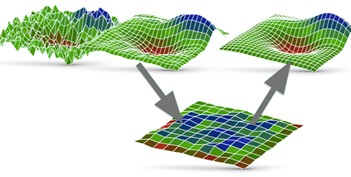
\includegraphics[height=5cm]{pics/es_multigrid.jpg}
		\caption{The V cycle in a multigrid method.}
		\label{fig:es_multigrid}
	\end{figure}




\subsection{Exercises}

{
\small

\begin{enumerate}
	
	\item Implement the LDLt decomposition using Matlab or similar software tools. Try it with a singular $A$ matrix: what causes the breakup of the method? 
	
	\item Implement the MINRES Krylov method using Matlab or similar software tools. Test it with randomly generated symmetric matrices. Generate a nearly singular matrix and plot the convergence. 
	
	\item Implement the preconditioned CG Krylov method using Matlab or similar software tools. Test it on random symmetric matrices using a diagonal preconditioner and later using an ILU preconditioner (you can reuse the ILU code in Matlab to avoid implementing the ILU) and show which is converging faster.
	
	\item Use a Krylov solver from the Matlab toolkit to solve randomly generated \textit{sparse} linear systems (or better a linear system generated from a FEA problem). Add the ILU preconditioner and see how the convergence improves. Force the ILU to exploit symmetry if any. Plot the convergence of the preconditioned Krylov method for decreasing ILU tolerance to fills-in creation, up to the case where ILU is forced to create no fills-in at all.
	
	
\end{enumerate}

}



\newpage
\section{Time integration}

Among the PDEs, there are some problems that depend on time. Studying the time evolution of such systems, starting from given 
initial conditions, is a numerical problem that can be solved via time integration. 

There are many different time integration 
methods (aka time steppers) which fit better some cases or others. 

Here we cannot present all of them, but we briefly 
discuss relevant aspects: the interested reader can find additional details in literature.

Classical textbooks about ODE time integration are \cite{hawa93,hawa96}. Further details on DAE time stepping schemes can be found in \cite{aspe98}.
The quite advanced topic of DVIs and MDIs can be approached using sources like \cite{pastew03dvi,pfeifferGlocker1996,acary2008numerical}.


\subsection{Classes of time-dependent problems}


In this section we introduce terminology and classifications for time-dependent problems.
Among these, the ODEs and DAEs represent by far the most relevant, and we urge the reader to 
understand their meaning. Remaining classes presented here, namely DIs, DVIs, MDIs are used
only in the more rare cases of problems subject to non-smooth set-valued laws, such as in
case of multibody systems with hard frictional contacts or simulation of analog electronic 
circuits with diods etc.


\subsubsection{ODEs}

Given a generic state $\vect{x}$ and time $t$, an \textit{Ordinary Differential Equation (ODE)} is a system of equations as:
%
\begin{align}
  \frac{d\vect{\vect{x}}}{dt}  = \vect{f} \left( \vect{x}, t\right)
\end{align}
%
together with prescribed initial conditions $\vect{x}(t_0)=\vect{x}_0$ 
\footnote{The expression above is the \textit{explicit form} of the ODE. One could express ODEs also in \textit{implicit form} as 
\[
\vect{F} \left( \frac{d\vect{\vect{x}}}{dt}, \vect{x}, t\right) = \vect{0}
\].
}.

An example: the transient heat equation \eqref{eq:transientheat} is an ODE with unknown $x$ as the temperature $T$, 
in fact it can be written as 
\[
\frac{\partial T}{\partial t} = \frac{1}{\rho c_p}\left(k\nabla^2 T + q\right)
\]
Solving such ODE means that one can obtain the time evolution of the temperature $T=T(\vect{x},t)$ for each point $\vect{x} \in \Omega$. Initial temperature
$\vect{T}(t_0)=\vect{T}_0$ must be prescribed as initial conditions.


The expression above is an ODE of \textit{index one}. Generic \textit{index-n} ODEs are in the form
%
\begin{align}
  \frac{d^n\vect{\vect{x}}}{dt^n}  = \vect{f} 
	\left( 
	\frac{d^{(n-1)}\vect{\vect{x}}}{dt^{(n-1)}},
	\ldots
	\frac{d^2\vect{\vect{x}}}{dt^2},
	\frac{d\vect{\vect{x}}}{dt},
	\vect{x}, t\right)
\end{align}

Its interesting to note that all index-n ODE can be converted into an index-one ODE by introducing a larger state with all the derivatives up to $n-1$ as in  $\vect{s}=\left\{\frac{d^{(n-1)}\vect{\vect{x}}}{dt^{(n-1)}}, \ldots, \frac{d^2\vect{\vect{x}}}{dt^2}, \frac{d\vect{\vect{x}}}{dt}, \vect{x} \right\}^T$ and rewriting it as:
%
\begin{align}
\frac{d\vect{\vect{s}}}{dt}  = 
\left\{
\begin{array}[pos]{c}
\frac{d^n\vect{\vect{x}}}{dt^n} \\
\ldots \\
\frac{d^2\vect{\vect{x}}}{dt^2} \\
\frac{d\vect{\vect{x}}}{dt}
\end{array}
\right\}
=
\left\{
\begin{array}[pos]{c}
\vect{f} 
	\left( 
	\frac{d^{(n-1)}\vect{\vect{x}}}{dt^{(n-1)}},
	\ldots
	\frac{d^2\vect{\vect{x}}}{dt^2},
	\frac{d\vect{\vect{x}}}{dt},
	\vect{x}, t\right) \\
\ldots \\
\frac{d^2\vect{\vect{x}}}{dt^2} \\
\frac{d\vect{\vect{x}}}{dt}
\end{array}
\right\};
\quad
\frac{d\vect{\vect{s}}}{dt}  = \vect{f}_s \left( \vect{s}, t\right)
\end{align}

An example is the index-2 ODE of unconstrained multibody dynamics: 
%
\begin{align}
  \matr{M} \frac{d\vect{\vect{v}}}{dt}  = \vect{f} \left( \vect{v},\vect{x}, t \right)  
	\label{eq:odemechanics}
\end{align}
%
that can be converted into a first-order ODE $\frac{d\vect{\vect{s}}}{dt}  = \vect{f}_s \left( \vect{s}, t \right)$ with $\vect{s} = \left\{ \vect{v}, \vect{x} \right\}$ and $\frac{d\vect{\vect{s}}}{dt}  = \left\{ \vect{a}, \vect{v} \right\} = \left\{ \matr{M}^{-1}\vect{f}(\vect{v},\vect{x}, t), \vect{v} \right\} = \vect{f}_s \left( \vect{s}, t \right)$.

This means that integration methods designed for first-order ODEs can be applied also to second-order ODEs without much work. However, this said, it is better to develop custom integrators for second-order ODEs when possible. %; this is the case of implicit integrators in \Chrono, for example.

The \textit{Picard-Lindelh\"{o}f theorem} states that for $\vect{f}\left( \vect{x}, t\right)$ uniformly Lipschitz continuous in $\vect{x}$ and continuous in $t$, there is an unique solution $\vect{x}(t)$ to the ODE for a given initial value. See also Cauchy–Lipschitz theorem.

For infinite-dimensional problems like the transient heat equation and similars, in most cases the ODE is expressed 
at the discretized level (look the section on weak formulation and discretization) 
so that one has a finite dimensional problem with a countable set of components in the unknown vector.



\subsubsection{DAEs}

Given a generic state $\vect{x}$, and time $t$, a \textit{Differential Algebraic Equation (DAE)} is a system of equations as:
%
\begin{align}
  \frac{d\vect{\vect{x}}}{dt}  &= \vect{f} \left( \vect{x}, \vect{y}, t\right) \\
	\vect{g} \left( \vect{x}, \vect{y}, t\right) &= \vect{0}
\end{align}
%
where $\vect{g}(.)$ is a set of constraint equations, also called \textit{geometric} or \textit{algebraic constraints}, and where $\vect{y}$ are the \textit{algebraic variables}.

The expression above is the \textit{semi-explicit form} of the DAE. One could express DAEs also in \textit{implicit form} as 
%
\begin{align}
\vect{F} \left( \frac{d\vect{\vect{x}}}{dt}, \vect{x}, \vect{y}, t\right) = \vect{0}
\end{align}
%
where the jacobian matrix $\frac{\partial \vect{F}}{\partial \vect{y}}$ is singular; in fact if it was singular, one could cast it as a simple ODE $\frac{d\vect{\vect{x}}}{dt}  = \vect{f} \left(\vect{x}, t\right)$.

The DAE \textit{initial conditions} cannot be provided as arbitrarily as in ODEs, because they must be \textit{consistent}, i.e. they must satisfy $\vect{F} \left( \frac{d\vect{\vect{x}}(t_0)}{dt}, \vect{x}(t_0), \vect{y}(t_0), t_0 \right) = \vect{0}$.

The \textit{differentiation index} of a DAE, or simply the \textit{index} of a DAE is the number of the differentiations that are required on the constraint equations of the semi-explicit form in order to obtain a pure ODE, after substitutions. An ODE is a DAE of index 0.

After index-reduction to an ODE, one might be tempted to perform the time integration of such ODE with classical integration schemes of ODEs. This might work for some steps but later some error tends to build up in the algebraic equations, giving a \textit{drift-off} phenomena in constraints. This because constraints would be satisfied only at the n-th derivative level (ex. acceleration, and not position) in the reduced ODE. To solve such drifting problem there are different methods. A rough approach is to introduce Baumgarte stabilization terms, like spring dampers that attracts the solution back on the manifold of the original, non differentiated constraints. Another approach is to satisfy constraints in implicit integrations methods specially crafted for DAEs, using Newton-Raphson solvers, and this is the case of HHT, generalized-$\alpha$ and other DAE-oriented implicit solvers.

An example: the incompressible Navier-Stokes equations are a DAE\footnote{Some authors call it a PDAE
to underline the (P)artial derivative differential algebraic equation nature, but it is only a matter of
terminology.} of index 2, where the constraints $\vect{g}(\vect{x},t) = \vect{0}$ are given
by the incompressibility constraint $\nabla \cdot \vect{u}=0$. 

An example: the index-2 DAE of constrained multibody dynamics
%
\begin{align}
  \matr{M} \frac{d\vect{\vect{v}}}{dt} - \matr{C}_q^T \vect{\lambda}  &= \vect{f} \left( \vect{q},\vect{v}, t \right)   \\
	\vect{C}(\vect{q},\vect{v},t) &=\vect{0} \\
	\dot{\vect{q}} &= \Gamma(\vect{q}) \vect{v}
	\label{eq:daemechanics}
\end{align}
%
with constraint reactions $\vect{\lambda}$, configuration $\vect{q}$, velocities $\vect{v}$, external and gyroscopic forces $\vect{f}$. 
Usually $\vect{v}=\dot{\vect{q}}$, but the complication of rotations in 3D might lead to the heterogeneous choice of using, say, quaternions in $\vect{q}$ and
angular velocities in $\vect{v}$, and this would require the linear operator $\Gamma$ for $\dot{\vect{q}} = \Gamma(\vect{q}) \vect{v}$.

\subsubsection{DIs}

A Filippov \textbf{Differential Inclusion} (DI) can be interpreted as an ODE 
for problems with discontinuous $\vect{f}(\vect{x},t)$:
\begin{equation}
\label{eq:FilippovDI}
\frac{d\vect{x}}{dt} \in \mathcal{F}\vect{f}(\vect{x},t) 
\quad
 \mathcal{F}f(\vect{x},t) = \bigcap_{\eta > 0} \bigcap_{N:\lambda_0(N)=0}
  \bar{\mathrm{co}} \vect{f}(\vect{x+\eta B_1}\setminus N,t)
\end{equation}
where $\lambda_0(E)$ is a Lebesgue measure on $E$, $B_1$ is a origin-centered 
unit ball, and $\vect{f}$ is discontinuous in $\vect{x}$. 

More in general, a \textit{Differential Inclusion} (DI) is a problem
\begin{equation}
\label{eq:DI}
\frac{d\vect{x}}{dt} \in \mathcal{F}(\vect{x},t) 
\end{equation}
where the set-valued function $\mathcal{F}(\vect{x},t)$ is
closed, bounded and convex and is upper semi-continuous, or
equivalently, $\mathcal{F}(\vect{x},t)$ has closed graph.


\subsubsection{DVIs}

We introduce \textbf{Differential Variational Inequality} (DVI) problems as:
\begin{subequations}
\label{eq:DVI}
\begin{align}
\frac{d\vect{x}}{dt} &= \vect{f}(\vect{x},\vect{u},t)  \\
\vect{u} &\in \mathsf{SOL}(\vect{F},\mathcal{K})
\end{align}
\end{subequations}
where $\mathsf{SOL}(\vect{F},\mathcal{K})$ is the (set of) solution 
to the VI$(\vect{F},\mathcal{K})$.
This is a special type of DI, too.
One can see that a DVI includes DAE as a special case: with $n$ bilateral
algebraic constraints one takes $\vect{F}$ as the vector of algebraic constraint residuals,
and uses $\mathcal{K}=\mathbb{R}^n$ so that $\vect{F}=\vect{0}$ everywhere by definition VI.


\subsubsection{MDIs}

A \textbf{Measure Differential Inclusion} (MDI) is a
generalization of DI (DVI) that also accomodates impulsive events. 
For second order problems as in mechanics, with 
$\vect{v}(t)=d\vect{q}/dt$
it reads:
\begin{equation}
\label{eq:MDI}
\frac{d\vect{v}}{dt} \in \mathcal{K}(\vect{q},t) 
\end{equation}
where $\vect{v}$ is a function of bounded variation and
$\mathcal{K}(\vect{q},t)$ is a set-valued function with
closed graph and closed convex values. 
The \textit{strong} definition of solution (Moreau) follows the singular
measure decomposition of $d\vect{v}=\vect{\nu}$ into 
$\vect{\nu}_s+\vect{h}\lambda_0$,
with respect to the singular part $\vect{\nu}_s$ 
and Lebesgue measure
$\lambda_0$ for continuous $\vect{h}(t) \in L^1(a,b)$: then the strong definition of solution is: 
$\vect{h}(t) \in \mathcal{K}(t)$ almost all $t$, and 
$d\vect{\nu}_s/|\vect{\nu}_s|(t) \in \mathcal{K}(t)_\infty$, 
i.e. the Radon-Nikodym derivative fits the horizon cone.
The \textit{weak} definition of solution (Stewart) is:
\begin{equation}
\label{eq:MDI_weak}
\frac{\int \phi(t) d\vect{\nu}(dt)}{ \int \phi(t) dt} 
 \in \bar{\mathrm{co}} \bigcup_{\tau:\phi(\tau)\neq 0} \mathcal{K}(\tau) 
\end{equation}
for any continuous $\phi(t):\mathbb{R}\rightarrow\mathbb{R}^+$ with compact support.





\subsection{Time integration numerical methods}

The goal is to provide methods that, given a state $\vect{x}_n$ at time $t_{n}$, can proceed to the next state at time $\vect{x}_{n+1}$ at time $t_{n+1}$ by advancing with a time step $h$, with $h=t_{n}-t_{n+1}$.

Focusing on ODEs only, for the moment, we can introduce some taxonomies of methods.

\begin{itemize}

\item
We can distinguish between \textbf{multistep} and \textbf{Runge\footnote{It is remarkable how many bright scientists attended the University of Göttingen.}-Kutta} methods.
The former depends on a history of previous timesteps in order to extrapolate a new one at the end of the new step, whereas the latter starts from the last timestep information then computes temporary intermediate $\vect{f}_j \left( \vect{x}_j, t\right)$ values after it, in order to compute the value at the end of the step.

\item
We can distinguish between \textbf{explicit} and \textbf{implicit} methods, the former using formulas that do not require any information on the value of state at the end of the step, whereas the latter uses (nonlinear) formulas that depend on the value of state at the end of the step, thus leading to more intricate solution schemes that rely on fixed point iterations or Newton iterations or in general iterative schemes that reach the solution at the end of the time step by iterating multiple times over a nonlinear set of equations. 
A notable feature of implicit methods is that they can solve problems with large stiffness (steep integrals with sudden rapid oscillations, so to speak) without the need of short time steps, whereas explicit methods require much shorter time steps to avoid divergence - see L-stability etc.

\item
We can distinguish between \textbf{fixed} time step or \textbf{variable} time step methods depend on the fact that, in the former case the time step $h$ is assumed constant, whereas in the second case the method can embed some smart heuristics to change the time step $h$ depending on its needs, for example making it shorter when approaching steepy stiff integrals, and making it larger when the time integration can proceed faster with lower CPU overhead. The latter case often involve the ability of un-doing and \textit{repeating the time step} with shorter $h$ when convergence or precision is not satisfactory. 
Think at this property as a simple add-on feature: almost all fixed step methods can be made of variable time step type by adding the rewinding capability to the original algorithms and adding some heuristics for shrinking/enlarging the time step.

\item
We mention that someone distinguishes between \textbf{stiff} and \textbf{non-stiff} methods, meaning the capability of handling problems with high stiffness without incurring in divergence. As this property is specific of implicit methods, often one can consider the class of stiff methods to be synonym of implicit methods. In a broader interpretation, one can use the term stiff also for explicit methods that, once embedded with some variable time step scheme, can attack (moderately) stiff problems by reducing automatically the time step up to avoid divergence.

\item
We also mention the not so frequent definition of \textbf{predictor-corrector} schemes. Rather than being a pure mathematical quality, this is an elaborate trick to help the convergence of sub-iterations of some implicit methods by warmstarting them with the help of another (often cheaper) integrator. In fact, in many predictor-corrector schemes, an explicit method is used to roughly estimate the new state working a bit like an extrapolator, and then an implicit integrator uses this estimate as a starting point for the refinement of the solution by running few Neton Raphson (or fixed point) iterations.

\end{itemize}

The qualities above are orthogonal, in the sense that a specific integration method could be, for example the backward Euler method is of Runge-Kutta type, implicit, usually with fixed time step, and stiff.

We present some relevant integration schemes in the following.


\subsubsection{Explicit Runge-Kutta methods}

These methods are based on multiple evaluation of the derivative at intermediate time steps, thus subdividing the $h$ time step into invisible temporary sub-steps.
The count of substeps is called \textit{stages}. The general formula for an \textbf{explicit Runge Kutta} method of $s$ stages is:
\begin{fleqn}
\begin{align}
\left[
\begin{aligned}
\vect{x}_{n+1} &= \vect{x}_n + h \sum_{i=1}^s b_i \vect{k}_i  \\
t_{n+1} &= t_n + h &
\end{aligned}
\right.
\end{align}
\end{fleqn}
with 
\begin{align}
 \vect{k}_1 & = \vect{f}(t_n, \vect{x}_n), \\
 \vect{k}_2 & = \vect{f}(t_n+c_2h, \vect{x}_n+h(a_{21}\vect{k}_1)), \\
 \vect{k}_3 & = \vect{f}(t_n+c_3h, \vect{x}_n+h(a_{31}\vect{k}_1+a_{32}\vect{k}_2)), \\
     & \ \ \vdots \\
 \vect{k}_s & = \vect{f}(t_n+c_sh, \vect{x}_n+h(a_{s1}\vect{k}_1+a_{s2}\vect{k}_2+\cdots+a_{s,s-1}\vect{k}_{s-1})).
\end{align}
where coefficients are given by a \textit{Butcher tableau}, satisfying $\sum_{j=1}^{i-1} a_{ij} = c_i \text{ for } i=2, \ldots, s.$

Among the explicit Runge-kutta methods, the most popular is the 4th order one, with $c_1=0, c_2=0.5, c_3=0.5, c_4=1, b_1=1/6, b_2=1/3, b_3=1/3, b_4=1/6$. 
It has a local truncation error on the order of $O ( h^5 )$. 

One can estimate the local error by performing a 5th order RK alongside the 4th order one, but to avoid
computing 4+5=9 functions $f()$, special methods such as the Runge-Kutta Fehlberg 4/5th order have been developed, that for the 5th order reuse 4 evaluations of $f()$ of the 4th order plus just one additional $f()$, that is used only for estimating the local error. A similar idea is used for Runge-Kutta 2/3 methods. These are known as ODE45 and ODE23 in Matlab or other packages.

Knowing an estimate of the local truncation error is useful for two reasons: for diagnostic during postprocessing, and/or to tell the integrator that the $h$ step is too large to give acceptable precision and therefore $h$ must be decreased or even re-done, if the integrator is of \textit{variable} time step type.


\subsubsection{Explicit Euler}

The \textbf{explicit Euler} method is a special type of explicit Runge-Kutta method, the simpliest one by the way. It boils down to:
\begin{fleqn}
\begin{align}
\left[
\begin{aligned}
\vect{x}_{n+1} &= \vect{x}_n + h \vect{f}(t_n, \vect{x}_n) \\
   t_{n+1} &= t_n + h 
\end{aligned}
\right.
\end{align}
\end{fleqn}

In terms of precision, it is a first-order method, thus it has a local truncation error on the order of $O ( h^2 )$ and its precision is a bit disappointing (even a simple parabolic ballistic trajectory will be approximated with growing error accumulation).

Moreover, large time steps in stiff problems will easily bring this method to divergence. 

The positive note, however, is that the explicit Euler method is very cheap in the computational sense, because it just requires one evaluation of the $\vect{f}(t_n, \vect{x}_n)$ term at each time step, given the current state $\vect{x}_n$.  Therefore, one can afford making very short time steps to circumvent its limitation on precision and to avoid the risk of divergence.


\subsubsection{Implicit Runge-Kutta methods}

The \textbf{implicit Runge-Kutta} methods are defined as:
\begin{fleqn}
\begin{align}
\left[
\begin{aligned}
\vect{x}_{n+1} &= \vect{x}_n + h \sum_{i=1}^s b_i\vect{k}_i \\
t_{n+1} &= t_n + h 
\end{aligned}
\right.
\end{align}
\end{fleqn}
%
with terms that depend on $\vect{x}_{n+1}$ as in
\begin{align}
\vect{k}_i = \vect{f}\left( t_n + c_i h,\ \vect{x}_{n} + h \sum_{j=1}^s a_{ij} \vect{k}_j \right), \quad i = 1, \ldots, s.
\end{align}


\subsubsection{Implicit Euler}

A very famous sub-case of implicit Runge-Kutta schemes is the \textbf{implicit Euler} (also known as backward Euler) method.
It is expressed as:
\begin{fleqn}
\begin{align}
\left[
\begin{aligned}
\vect{x}_{n + 1} &= \vect{x}_n + h f(t_n + h,\ \vect{x}_{n + 1}) \\
t_{n+1} &= t_n + h 
\end{aligned}
\right.
\end{align}
\end{fleqn}

Note here a typical complication of all implicit methods: a system of (possibly nonlinear) algebraic equations has 
to be solved to compute $\vect{x}_{n + 1}$, and this must happen at each time step.



\subsubsection{Adams-Bashforth methods}

This is an example from the class of multistep methods. As for all multisteps methods, it requires an history of previous time steps. 

Recycling the information of previous time steps will help the precision with low computational cost - consider that Runge-Kutta methods achieve accuracy at the cost of computing intermediate time steps that are discarded. However it also leads to some issues, one being the fact that they require some tricks in starting them from scratch, when previous time history is not given.

The Adams-Bashforth methods of order $s$ are explicit methods given by the general linear multistep formula:
\begin{fleqn}
\begin{align}
\left[
\begin{aligned}
\sum_{j=0}^s a_j \vect{x}_{n+j} &= h\sum_{j=0}^s b_j \vect{f}(t_{n+j},\vect{x}_{n+j}) \\
t_{n+1} &= t_n + h 
\end{aligned}
\right.
\end{align}
\end{fleqn}
where one has $a_s=-1$, $a_j=0$ for $j<s$, and $b_j$ coefficients are given by a Lagrange polynomial interpolation hence $b_{s-j-1} = \frac{(-1)^j}{j!(s-j-1)!} \int_0^1 \prod_{i=0 \atop i\ne j}^{s-1} (u+i) \,du, \qquad \text{for } j=0,\ldots,s-1$, since the method is explicit $b_s=0$; for example the 4-th order Adams-Bashforth boils down to 
\begin{fleqn}
\begin{align}
\left[
\begin{aligned}
\vect{x}_{n+4} &= \vect{x}_{n+3} + h\left( \frac{55}{24} \vect{f}(t_{n+3}, \vect{x}_{n+3}) - \frac{59}{24} \vect{f}(t_{n+2}, \vect{x}_{n+2}) + \frac{37}{24} \vect{f}(t_{n+1}, \vect{x}_{n+1}) - \frac{9}{24} \vect{f}(t_n, \vect{x}_n) \right) \\
t_{n+1} &= t_n + h 
\end{aligned}
\right.
\end{align}
\end{fleqn}
and one can see that it can reuse three previous $\vect{f}$ informations each time it advances one $h$ step.

Adams-Bashforth methods with $s$ steps have local truncation error on the order of $O ( h^{(s+1)} )$.






\subsubsection{Adams-Moulton methods}

This is another class of linear multistep methods, similar to Adams-Bashforth, but this time it is an implicit integration.
For example, the 4-th order Adams-Moulton method boils down to:
\begin{fleqn}
\begin{align}
\left[
\begin{aligned}
\vect{x}_{n+3} &= \vect{x}_{n+2} + h \left( \frac{9}{24} \vect{f}(t_{n+3},\vect{x}_{n+3}) + \frac{19}{24} \vect{f}(t_{n+2},\vect{x}_{n+2}) - \frac{5}{24} \vect{f}(t_{n+1},\vect{x}_{n+1}) + \frac{1}{24} \vect{f}(t_n,\vect{x}_n) \right) \\
t_{n+1} &= t_n + h 
\end{aligned}
\right.
\end{align}
\end{fleqn}
and one can see that the $\vect{f}(t_{n+3},\vect{x}_{n+3})$ terms depends on the state at the end of the time step $\vect{x}_{n+3}$, making it an implicit method (and consequently requiring some complicate machinery like Newton-Raphson iterations to solve for $\vect{x}_{n+3}$).

Adams-Moulton methods with $s$ steps have order $s+1$ and local truncation error of order $O ( h^{(s+2)} )$.


\subsubsection{Trapezoidal method}

The trapezoidal integrator is in implicit integrator, and it can be seen both as a special case of Adams-Moulton integrator with one step, or an implicit Runge-Kutta of 2nd order. After the impicit Euler, it is perhaps the simplest implicit integration scheme.
The scheme is:
\begin{fleqn}
\begin{align}
\left[
\begin{aligned}
\vect{x}_{n+1} &= \vect{x}_n + \tfrac12 h \left( \vect{f}(t_n,\vect{x}_n) + \vect{f}(t_{n+1},\vect{x}_{n+1} \right) \\
t_{n+1} &= t_n + h 
\end{aligned}
\right.
\end{align}
\end{fleqn}
This method has order 2, local truncation error of order $O ( h^{(s+2)} )$. The method unstable even if it is unconditionally stable. 

Among the implicit methods, it stands out because it does not introduce numerical damping, but this property is less usable than it seems in practical scenarios with strong nonlinearities that can create divergence (the unconditional stability holds in the theoretical ideal case of linear stiffness) so a bit of numerical damping in implicit integrators would be welcome anyway.


\subsubsection{BDF methods}

These are implicit linear multistep methods, but are a bit simplier and more efficient than the Adams-Moulton methods. The general formula for an order-$s$ BDF scheme is:
\begin{fleqn}
\begin{align}
\left[
\begin{aligned}
\sum_{k=0}^s a_k \vect{x}_{n+k} &= h \beta \vect{f}(t_{n+s}, \vect{x}_{n+s}) \\
t_{n+1} &= t_n + h 
\end{aligned}
\right.
\end{align}
\end{fleqn}
with properly chosen coefficients $\beta$ and $a_k$.

The implicit Euler is also the special case of BDF with order one. We mention here the coefficients for other orders:
\begin{itemize}
	\item second order BDF: 
	\[
	\vect{x}_{n+2} - \tfrac43 \vect{x}_{n+1} + \tfrac13 \vect{x}_n = \tfrac23 h \vect{f}(t_{n+2}, \vect{x}_{n+2})
	\]
	\item third order BDF: 
	\[
	\vect{x}_{n+3} - \tfrac{18}{11} \vect{x}_{n+2} + \tfrac9{11} \vect{x}_{n+1} - \tfrac2{11} \vect{x}_n = \tfrac6{11} h \vect{f}(t_{n+3}, \vect{x}_{n+3})
	\]
	\item fourth order BDF: 
	\[
	\vect{x}_{n+4} - \tfrac{48}{25} \vect{x}_{n+3} + \tfrac{36}{25} \vect{x}_{n+2} - \tfrac{16}{25} \vect{x}_{n+1} + \tfrac{3}{25} \vect{x}_n = \tfrac{12}{25} h \vect{f}(t_{n+4}, \vect{x}_{n+4})
	\]
\end{itemize}

Note that linear multistep methods with an order greater than 2 cannot be A-stable (see stability).



\subsection{Numerical implementation of methods}

In the previous section we presented some of the most relevant integration schemes, but in a general setting that assumes an index-1 ODE, without telling how to perform the Newton-Raphson substeps for the implicit methods, and telling nothing about DAEs. 

In a practical setting, however, one should better exploit the structure of the problem at hand. For example, in mechanics, it is true that one can turn an order-2 ODE (with accelerations) into an index-1 ODE grouping positions and speeds in a single state $\vect{x}=(\vect{q},\vect{v})$, however it is better to express the method directly at the level of index-2 ODE with separate equations for speeds and accelerations. This also makes easier to recover the jacobian matrices for the implicit methods that require Newton-Raphson iterations.

Moreover, what can be done in case of DAEs, that is when algebraic constraints are added to ODEs?

In this section we show, for a limited set of integrators, how to implement them at the algorithmical level, also showing some schemes for DAEs.


\subsubsection{Trapezoidal, for index-2 ODE}

For simplicity, let's start with the ODE case, i.e. also a DAE where no constraints are present.


For an index-2 ODE as used in dynamics in \label{eq:odemechanics} (btw the DAE case will be dealt later), we use state 
$\vect{x}=\left\{ \vect{q},\vect{v} \right\}$, $\dot{\vect{x}}=\left\{ \vect{v},\vect{a} \right\}$ so we have:


\begin{empheq}[left=\empheqlbrack]{align}
\vect{q}^{l+1}-\vect{q}^l - \left( \frac{\vect{v}^{l+1}+\vect{v}^l}{2} \right) h = 0
\label{eq:trapzoidal_q}
\\
\vect{v}^{l+1}-\vect{v}^l - \left( \frac{\vect{a}^{l+1}+\vect{a}^l}{2} \right) h = 0
\label{eq:trapzoidal_v} \\
t^{l+1} = t^l + h
\end{empheq}


In general one has computable $\vect{a}^{l}$ and $\vect{a}^{l+1}$, where in sake of compactness we 
write
$\vect{a}^{l}$ for $\vect{a}(\vect{q}^{l},\vect{v}^{l},t^{l})$, as well as 
$\vect{a}^{l+1}$ for $\vect{a}(\vect{q}^{l+1},\vect{v}^{l+1},t^{l+1})$.
Given that in a mechanical context one splits $\vect{f}=\matr{M} \vect{a}$, 
one can also write the following (that fits in ODE too) where for brevity we write 
$\vect{f}^{l}$ for $\vect{f}(\vect{q}^{l},\vect{v}^{l},t^{l})$, as well as 
$\vect{f}^{l+1}$ for $\vect{f}(\vect{q}^{l+1},\vect{v}^{l+1},t^{l+1})$, :

\begin{align}
\vect{q}^{l+1}-\vect{q}^l - \left( \frac{\vect{v}^{l+1}+\vect{v}^l}{2} \right) h = 0
\label{eq:trapzoidal_q2}
\\
\left( \vect{v}^{l+1}-\vect{v}^l \right) \left( \matr{M}^{l+1}+\matr{M}^{l} \right) - h \vect{f}^{l+1} -h \vect{f}^l = 0
\label{eq:trapzoidal_v2}
\end{align}

Let's call $\vect{G}=\left\{ \vect{G}_q, \vect{G}_v \right\}$ the residual of the system above. 
To satisfy $\vect{G}=0$, one can use a Newton-Raphson iteration (the subscribt means the iteration number) and solve 
for the proper $\vect{q}^{l+1},\vect{v}^{l+1}$:

\begin{align}
\vect{G}(\vect{q}^{l+1},\vect{v}^{l+1}) = 0 \\
\vect{G}(\vect{q}^{l+1}_n,\vect{v}^{l+1}_n) + 
\left[ 
\begin{array}[pos]{cc}
	\frac{\partial \vect{G}_q}{\partial \vect{q}} & \frac{\partial \vect{G}_q}{\partial \vect{v}}  \\
	\frac{\partial \vect{G}_v}{\partial \vect{q}} & \frac{\partial \vect{G}_v}{\partial \vect{v}} 
\end{array}
 \right]_n^{l+1} 
\left\{ 
\begin{array}[pos]{c}
	\vect{q}^{l+1}_{n+1} - \vect{q}^{l+1}_{n} \\ 
	\vect{v}^{l+1}_{n+1} - \vect{v}^{l+1}_{n}
\end{array}
 \right\}
 = 0  
\end{align}
%
also using deltas as a more compact notation for corrections:
\begin{align}
\vect{G}(\vect{q}^{l+1}_n,\vect{v}^{l+1}_n) + \left[ 
\begin{array}[pos]{cc}
	\frac{\partial \vect{G}_q}{\partial \vect{q}} & \frac{\partial \vect{G}_q}{\partial \vect{v}}  \\
	\frac{\partial \vect{G}_v}{\partial \vect{q}} & \frac{\partial \vect{G}_v}{\partial \vect{v}} 
\end{array}
 \right]_n^{l+1}
\left\{  
\begin{array}[pos]{c}
	\Delta\vect{q}^{l+1} \\ 
	\Delta\vect{v}^{l+1}
\end{array}
 \right\} 
 = 0  
\label{eq:trapzoidal_qv}
\end{align}
%

or, in a even more compact notation for jacobian $\matr{J}$, it boils down to a Newton-Raphson step of the type 
\begin{align}
\matr{J}
\left\{ 
\begin{array}[pos]{c}
	\Delta\vect{q}^{l+1} \\ 
	\Delta\vect{v}^{l+1}
\end{array}
 \right\} 
 = -\vect{G}(\vect{q}^{l+1}_n,\vect{v}^{l+1}_n)
\end{align}

Now, note that a straight implementation of the above NR step is not efficient since $J$ would be highly sparse and unsymmetric. 
One can unroll the equations, and from Eq.\ref{eq:trapzoidal_q} one gets
$\Delta\vect{q}^{l+1}=\frac{h}{2}\Delta\vect{v}^{l+1}$, that allows 
	\footnote{The fact that $\Delta\vect{q}^{l+1}=\frac{h}{2}\Delta\vect{v}^{l+1}$ is used in various literature, 
	but it is true only close to the solution, when 
	the residual $\vect{G}_q$ is close to zero, 
	otherwise it would be 
	$\Delta\vect{q}^{l+1}=\frac{h}{2}\Delta\vect{v}^{l+1}-\vect{G}_q = \frac{h}{2}\Delta\vect{v}^{l+1} -\vect{q}^{l+1}+\vect{q}^l + \left( \frac{\vect{v}^{l+1}+\vect{v}^l}{2} \right) h$. However this might overly complicate the NR step that follows. } 
to rewrite as: 

\begin{align}
\matr{J} = 
\left[ 
\begin{array}[pos]{cc}
	\frac{\partial \vect{G}_q}{\partial \vect{q}} & \frac{\partial \vect{G}_q}{\partial \vect{v}}  \\
	\frac{\partial \vect{G}_v}{\partial \vect{q}} & \frac{\partial \vect{G}_v}{\partial \vect{v}} 
\end{array}
 \right]_n^{l+1}
 = 
\left[ 
\begin{array}[pos]{cc}
	\matr{I} & -\frac{h}{2} \matr{I}  \\
	-h \nabla_q \vect{f}^{l+1}  & (M^{l+1}+ M^l) -h \nabla_v \vect{f}^{l+1}
\end{array}
 \right] 
\end{align}

Now one can put that jacobian in Eq.\ref{eq:trapzoidal_qv}, develop the equations and arrange them so that one can write the step Eq.\ref{eq:trapzoidal_qv} as three substeps to be repeated in sequence for each Newton iteration, until $\Delta\vect{q}^{l+1}$ and $\Delta\vect{v}^{l+1}$ go to zero. 
In such steps we define $\left( \frac{\matr{M}^{l+1}+\matr{M}^l}{2} \right) = \hat{\matr{M}}$, that is often the constant mass $\matr{M}$ in many cases. 
One gets the Newton step procedure:


\begin{empheq}[box=\fbox]{align}
\left[ \hat{\matr{M}} - \frac{h^2}{4} \nabla_q \vect{f}^{l+1} - \frac{h}{2} \nabla_v \vect{f}^{l+1} \right] \Delta\vect{v}^{l+1} &=
\left( \vect{v}^{l}-\vect{v}^{l+1} \right) \hat{\matr{M}} + \frac{h}{2} \vect{f}^{l} + \frac{h}{2} \vect{f}^{l+1} 
\label{eq:trapzoidal_qv1}
\\
\vect{v}^{l+1}_{n+1} &= \vect{v}^{l+1}_{n} + \Delta\vect{v}^{l+1}
\label{eq:trapzoidal_qv2}
\\
\vect{q}^{l+1} &= \vect{q}^{l} + \left( \frac{\vect{v}^{l+1}_{n+1} + \vect{v}^{l}}{2} \right) h
\label{eq:trapzoidal_qv3}
\end{empheq}
%
where only the 1st step Eq.\ref{eq:trapzoidal_qv1} is the computationally intensive step. But the matrix is hermitian, at least.

\begin{itemize}

	\item Note that the residual in Eq.\ref{eq:trapzoidal_qv1} is the same residual of Eq.\ref{eq:trapzoidal_v2}, except everything is divided by a factor 2 for convenience.
	
	\item Note that if the exact expression $\Delta\vect{q}^{l+1}=\frac{h}{2}\Delta\vect{v}^{l+1}-\vect{G}_q$ is used, the term $-\vect{G}_q$ must modify the residual in Eq.\ref{eq:trapzoidal_qv1} by adding $... + \frac{h}{2} \nabla_q \vect{f}^{l+1} \vect{G}_q$ that is $... + \frac{h}{2} \nabla_q \vect{f}^{l+1} \left( \vect{q}^{l+1}-\vect{q}^l - \left( \frac{\vect{v}^{l+1}+\vect{v}^l}{2} \right) h \right)$.
	
	\item Note that $\nabla_q \vect{f}$ is $-\matr{K}$, the stiffness matrix in structural elments, and $\nabla_v \vect{f}$ is $-\matr{R}$, the damping matrix.

	
\end{itemize}





\subsubsection{Euler implicit, for index-2 ODE}

The Euler implicit method (backward Euler), for a 2nd order ODE, is:

\begin{empheq}[left=\empheqlbrack]{align}
\vect{q}^{l+1}-\vect{q}^l - \vect{v}^{l+1} h = 0
\label{eq:euler_q}
\\
\vect{v}^{l+1}-\vect{v}^l - \vect{a}^{l+1} h = 0
\label{eq:euler_v} 
\\
t^{l+1}= t^l + h
\end{empheq}

Again, as with the trapezoidal, this can be solved with a Newton-Raphson iteration.
Let's call $\vect{G}=\left\{ \vect{G}_q, \vect{G}_v \right\}$ the residual of the system above. 
%
\begin{align}
\matr{J}
\left\{ 
\begin{array}[pos]{c}
	\Delta\vect{q}^{l+1} \\ 
	\Delta\vect{v}^{l+1}
\end{array}
 \right\} 
 = -\vect{G}(\vect{q}^{l+1}_n,\vect{v}^{l+1}_n)
\end{align}
%
where the jacobian, in this case, is:
%
\begin{align}
\matr{J} = 
\left[ 
\begin{array}[pos]{cc}
	\frac{\partial \vect{G}_q}{\partial \vect{q}} & \frac{\partial \vect{G}_q}{\partial \vect{v}}  \\
	\frac{\partial \vect{G}_v}{\partial \vect{q}} & \frac{\partial \vect{G}_v}{\partial \vect{v}} 
\end{array}
 \right]_n^{l+1}
 = 
\left[ 
\begin{array}[pos]{cc}
	\matr{I} & -h\matr{I}  \\
	-h \nabla_q \vect{f}^{l+1}  & \hat{\matr{M}} -h \nabla_v \vect{f}^{l+1}
\end{array}
 \right] 
\end{align}

Also in this case we defined $\left( \frac{\matr{M}^{l+1}+\matr{M}^l}{2} \right) = \hat{\matr{M}}$, that is often the constant mass $\matr{M}$ in many cases. 
By developing the expression above and by setting $\Delta\vect{q}^{l+1}=h \Delta\vect{v}^{l+1}$  one gets the Newton step procedure:


\begin{empheq}[box=\fbox]{align}
\left[ \hat{\matr{M}} - h^2 \nabla_q \vect{f}^{l+1} - h \nabla_v \vect{f}^{l+1} \right] \Delta\vect{v}^{l+1} &=
\left( \vect{v}^{l}-\vect{v}^{l+1} \right) \hat{\matr{M}} + h \vect{f}^{l+1} 
\label{eq:euler_qv1}
\\
\vect{v}^{l+1}_{n+1} &= \vect{v}^{l+1}_{n} + \Delta\vect{v}^{l+1}
\label{eq:euler_qv2}
\\
\vect{q}^{l+1} &= \vect{q}^{l} + h \vect{v}^{l+1}_{n+1} 
\label{eq:euler_qv3}
\end{empheq}

Some remarks here.

\begin{itemize}

	\item 
	In Eq.\ref{eq:euler_qv3} one could use $\Delta\vect{q}^{l+1}=h \Delta\vect{v}^{l+1}$ and rather write 
	$\vect{q}^{l+1}_{n+1} = \vect{q}^{l+1}_{n} + h \Delta\vect{v}^{l+1}_{n+1}$, but this is questionable.
	
	\item 
	The single first step of this NR process is exactly the Euler semi-implicit DVI in Chrono::Engine
	(not considering the constraints and contacts, here) because 
	one can express it with unknowns $\vect{v}^{l+1}_{n+1}$ rather than deltas, so it can be also:
%
\begin{align}
\left[ \hat{\matr{M}} - h^2 \nabla_q \vect{f}^{l+1} - h \nabla_v \vect{f}^{l+1} \right] \vect{v}^{l+1}_{n+1} &= 
\left[ \hat{\matr{M}} - h^2 \nabla_q \vect{f}^{l+1} - h \nabla_v \vect{f}^{l+1} \right] \vect{v}^{l+1}_{n} + \nonumber \\
& + \left( \vect{v}^{l}-\vect{v}^{l+1} \right) \hat{\matr{M}} + h \vect{f}^{l+1} 
\label{eq:euler_qv1b}
\\
\vect{q}^{l+1} &= \vect{q}^{l} + \vect{v}^{l+1}_{n+1} h
\label{eq:euler_qv2b}
\end{align}
%
and then, if at the first step we set $\vect{v}^{l+1}_0 = \vect{v}^{l}$, and assuming $\vect{f}^{l+1} \approx \vect{f}^{l}$, we simply get:
%
\begin{align}
\left[ \hat{\matr{M}} - h^2 \nabla_q \vect{f}^{l+1} - h \nabla_v \vect{f}^{l+1} \right] \vect{v}^{l+1} &= 
\left[ \hat{\matr{M}} - h^2 \nabla_q \vect{f}^{l+1} - h \nabla_v \vect{f}^{l+1} \right] \vect{v}^{l} + h \vect{f}^{l} 
\label{eq:euler_qv1c}
\\
\vect{q}^{l+1} &= \vect{q}^{l} + \vect{v}^{l+1}_{n+1} h
\label{eq:euler_qv2c}
\end{align}
%
(just by removing the stiffness and damping matrices $\nabla_q \vect{f}^{l+1}$, $\nabla_v \vect{f}^{l+1}$ if there are no finite elements, and by adding jacobians to satisfy bilateral constraints, one turns Eq.\ref{eq:euler_qv1c} into the same problem solved by the DVI timestepper of Chrono::Engine if without unilateral constraints)

\end{itemize}




\subsubsection{Euler implicit, for DAE}


Let's consider an index-2 DAE as in constrainted multibody mechanics, see \eqref{eq:daemechanics}.

There are different options for the DAE solution, for instance use constraints in DAE implicit form $F()$ to solve with Newton-Raphson, or do not solve them monolithically with DAE but just do projections on the manifold at each Newton iteration, etc. 
Here we enforce constraints (at the end of the time step) using a Newton-Raphson iteration, together with the Euler first order approximation used in the constraint-less case.

Add constraints $\vect{C}(\vect{q},t)=\vect{0}$. 
For brevity, denote 
\begin{align}
\matr{C}_q &= \nabla_q \vect{C}^T =  \frac{\partial \vect{C}}{\partial \vect{q}} \\
\matr{C}_t &= \nabla_t \vect{C}^T =  \frac{\partial \vect{C}}{\partial t}
\end{align}
Also, in sake of compactness we write
$\vect{C}^{l}$ for $\vect{C}(\vect{q}^{l},t^{l})$, as well as 
$\vect{C}^{l+1}$ for $\vect{C}(\vect{q}^{l+1},t^{l+1})$.

The Euler implicit method (backward Euler), for DAE with constraints satisfied at the end of timestep, is:

\begin{empheq}[left=\empheqlbrack]{align}
\vect{q}^{l+1}-\vect{q}^l - \vect{v}^{l+1} h = 0
\label{eq:eulerDAE_q}
\\
\hat{\matr{M}}(\vect{v}^{l+1}-\vect{v}^l) - h \vect{f}^{l+1} - h \matr{C}_q^T \vect{\lambda}^{l+1} = 0
\label{eq:eulerDAE_v}
\\
\vect{C}(\vect{q}^{l+1},t^{l+1}) = \vect{0}
\label{eq:eulerDAE_c}
\\
t^{l+1} = t^l + h
\end{empheq}

Let's call $\vect{G}=\left\{ \vect{G}_q, \vect{G}_v, \vect{G}_c \right\}$ the residual of the system above.
Solving with a Newton-Raphson iteration: 
%
\begin{align}
\left[ 
\begin{array}[pos]{ccc}
\matr{I} & -h\matr{I} & 0 \\
	-h \nabla_q \vect{f}^{l+1}  & \hat{\matr{M}} -h \nabla_v \vect{f}^{l+1} & - h \matr {C}_q^T  \\
	\matr {C}_q & 0 & 0
\end{array}
 \right]
\left\{ 
\begin{array}[pos]{c}
	\Delta\vect{q}^{l+1} \\ 
	\Delta\vect{v}^{l+1} \\ 
	\Delta\vect{\lambda}^{l+1}
\end{array}
 \right\} 
 = -\vect{G}
\end{align}
%

By developing the expression above and by setting $\Delta\vect{q}^{l+1}=\frac{h}{2}\Delta\vect{v}^{l+1}$ (see footnote in previous page) 
one gets the 'unrolled' Newton step procedure, where the hard part is the 1st step, the classical saddle-point problem:


\begin{empheq}[box=\fbox]{align}
\left[
\begin{array}[pos]{cc}
\left[ \hat{\matr{M}} - h^2 \nabla_q \vect{f}^{l+1} - h \nabla_v \vect{f}^{l+1} \right] & \matr{C}_q^T \\ 
\matr{C}_q & 0
\end{array}
\right] 
&
\left\{
\begin{array}[pos]{c}
\Delta\vect{v}^{l+1} \\
-h \Delta\vect{\lambda}^{l+1}
\end{array}
\right\}
 = \nonumber \\
 \left\{
\begin{array}[pos]{c}
\left( \vect{v}^{l}-\vect{v}^{l+1} \right) \hat{\matr{M}} + h \vect{f}^{l+1} + h \matr{C}_q^T \vect{\lambda}^{l+1} \\
\frac{\vect{C}^{l+1}}{h}
\end{array}
\right\} &
\label{eq:eulerDAE_qv1}
\\
\vect{v}^{l+1}_{n+1} &= \vect{v}^{l+1}_{n} + \Delta\vect{v}^{l+1}
\label{eq:eulerDAE_qv2}
\\
\vect{\lambda}^{l+1}_{n+1} &= \vect{\lambda}^{l+1}_{n} + \Delta\vect{\lambda}^{l+1}
\label{eq:eulerDAE_qv3}
\\
\vect{q}^{l+1} &= \vect{q}^{l} + h \vect{v}^{l+1}_{n+1} 
\label{eq:eulerDAE_qv4}
\end{empheq}




\subsubsection{Trapezoidal, for DAE}


A possibility is to add to Eqs. \ref{eq:trapzoidal_q2} and \ref{eq:trapzoidal_v2} the following constraint that requires positions to be satisfied at the end of the step:
\[
\vect{C}(\vect{q}^{l+1},t^{l+1})=\vect{0}
\] 
and add reaction forces $\vect{\lambda}$ too, as $\vect{f} + \nabla_v \vect{C} \vect{\lambda} =\matr{M}\vect{a} $.
This leads to the following trapezoidal rule for DAE:

\begin{empheq}[left=\empheqlbrack]{align}
\vect{q}^{l+1}-\vect{q}^l - \left( \frac{\vect{v}^{l+1}+\vect{v}^l}{2} \right) h = 0
\label{eq:trapzoidal_q3}
\\
\left( \vect{v}^{l+1}-\vect{v}^l \right) \left( \matr{M}^{l+1}+\matr{M}^{l} \right) - h \vect{f}^{l+1} -h \vect{f}^l  
- h \nabla_v \vect{C}^{l} \vect{\lambda}^{l} - h \nabla_v \vect{C}^{l+1} \vect{\lambda}^{l+1}= 0
\label{eq:trapzoidal_v3}
\\
\vect{C}(\vect{q}^{l+1},t^{l+1})=\vect{0}
\label{eq:trapzoidal_c3}
\\
t^{l+1} = t^l +h
\end{empheq}

This done, one can express a Newton-Raphson process to compute the unknowns $\vect{v}^{l+1}$, $\vect{v}^{l+1}$, $\vect{\lambda}^{l+1}$ that give a zero residual $\vect{G}$ for the three equations above:
%
\begin{align}
\left[ 
\begin{array}[pos]{ccc}
\matr{I} & -\frac{h}{2}\matr{I} & 0 \\
	-\frac{h}{2} \nabla_q \vect{f}^{l+1}  & \hat{\matr{M}} -\frac{h}{2} \nabla_v \vect{f}^{l+1} &  -\frac{h}{2} \matr {C}_q^{l+1,T}  \\
	\matr {C}_q^{l+1} & 0 & 0
\end{array}
 \right]
\left\{ 
\begin{array}[pos]{c}
	\Delta\vect{q}^{l+1} \\ 
	\Delta\vect{v}^{l+1} \\ 
	\Delta\vect{\lambda}^{l+1}
\end{array}
 \right\} 
 = -\vect{G}
\end{align}

This can be unrolled to work with a more friendly linear system with hermitian matrix and two following uncoupled steps:

\begin{empheq}[box=\fbox]{align}
&
\left[
\begin{array}[pos]{cc}
\left[ \hat{\matr{M}} - \frac{h^2}{4} \nabla_q \vect{f}^{l+1} - \frac{h}{2} \nabla_v \vect{f}^{l+1} \right] & \matr {C}_q^{l+1,T} \\ 
\matr {C}_q^{l+1} & 0
\end{array}
\right] 
\left\{
\begin{array}[pos]{c}
\Delta\vect{v}^{l+1} \\
-\frac{h}{2} \Delta\vect{\lambda}^{l+1}
\end{array}
\right\}
 = \nonumber \\
& 
 \left\{
\begin{array}[pos]{c}
\left( \vect{v}^{l}-\vect{v}^{l+1} \right) \hat{\matr{M}} 
+ \frac{h}{2}\left( \vect{f}^{l} + \vect{f}^{l+1} + \matr{C}_q^{l,T} \vect{\lambda}^{l} + \matr{C}_q^{l+1,T} \vect{\lambda}^{l+1} \right) \\
\frac{1}{h}\vect{C}^{l+1}
\end{array}
\right\} 
\label{eq:trapezDAE_qv1}
\\ &\quad
\vect{v}^{l+1}_{n+1} = \vect{v}^{l+1}_{n} + \Delta\vect{v}^{l+1}
\label{eq:trapexDAE_qv2}
\\ &\quad
\vect{\lambda}^{l+1}_{n+1} = \vect{\lambda}^{l+1}_{n} + \Delta\vect{\lambda}^{l+1}
\label{eq:trapezDAE_qv3}
\\ &\quad
\vect{q}^{l+1} = \vect{q}^{l} + \frac{h}{2} \left( \vect{v}^{l} + \vect{v}^{l+1}_{n+1} \right)
\label{eq:trapezDAE_qv4}
\end{empheq}



\subsubsection{Newmark, for ODE and DAE}


The Newmark family of second-order integrators is very popular in the FEM community. 

One has

\begin{empheq}[left=\empheqlbrack]{align}
\vect{q}^{l+1}-\vect{q}^l - h \vect{v}^l - \frac{h^2}{2} \left[ (1-2\beta) \vect{a}^l + 2\beta \vect{a}^{l+1} \right]  = 0
\label{eq:newmark_q}
\\
\vect{v}^{l+1}-\vect{v}^l - h \left[(1-\gamma) \vect{a}^l + \gamma \vect{a}^{l+1} \right]= 0
\label{eq:newmark_v}
\\
\matr{M} \vect{a}^{l+1} + (\matr{C}_q^T\vect{\lambda}-\vect{f})^{l+1}  = 0
\label{eq:newmark_a}
\\
t^{l+1} = t^l + h
\end{empheq}

Different values of the $\gamma$ and $beta$ parameters provide different behaviors.
\begin{itemize}
	\item The $\gamma$ parameter usually ranges in the $[1/2, 1]$ interval. 
	\item For $\gamma = 1/2$, no numerical damping.
	\item For $\gamma > 1/2$, numerical damping increases.
	\item The $\beta$ parameter usually ranges in the $[0, 1]$ interval.
	\item For $\beta = 1/4, \gamma = 1/2$ one gets the constant acceleration method.
	\item For $\beta = 1/6, \gamma = 1/2$ one gets the linear acceleration method.
	\item The method is second order accurate only for $\gamma = 1/2$.
\end{itemize}

For this type of method, considering constraints being enforced in the DAE, the Newton iteration is represented again by a linear problem, this time in accelerations:


\begin{empheq}[box=\fbox]{align}
&
\left[
\begin{array}[pos]{cc}
 \matr{H} & \matr{\overline{C}}_q^T \\ 
\matr{\overline{C}}_q & 0
\end{array}
\right] 
\left\{
\begin{array}[pos]{c}
\Delta\vect{a}^{l+1} \\
\Delta\vect{\lambda}^{l+1}
\end{array}
\right\}
 = \nonumber \\
& 
 \left\{
\begin{array}[pos]{c}
\matr{M}\vect{a}^{l+1}
+ (\matr{C}_q^T\vect{\lambda}-\vect{f})^{l+1} 
\\
\frac{1}{\beta h^2}\vect{C}^{l+1}
\end{array}
\right\} 
\label{eq:newmark_qv1}
\\ &\quad
\vect{a}^{l+1}_{n+1} = \vect{a}^{l+1}_{n} + \Delta\vect{a}^{l+1}
\label{eq:newmark_qv2}
\\ &\quad
\vect{\lambda}^{l+1}_{n+1} = \vect{\lambda}^{l+1}_{n} + \Delta\vect{\lambda}^{l+1}
\label{eq:newmark_qv3}
\\ &\quad
\vect{v}^{l+1} = \vect{v}^l + h \left[(1-\gamma) \vect{a}^l + \gamma \vect{a}^{l+1} \right]
\label{eq:newmark_qv4}
\\ &\quad
\vect{q}^{l+1} = \vect{q}^l + h \vect{v}^l + \frac{h^2}{2} \left[ (1-2\beta) \vect{a}^l + 2\beta \vect{a}^{l+1} \right] 
\label{eq:newmark_qv5}
\end{empheq}
 
where 
\[
\matr{H} = 
\left[
\matr{M}
- \gamma h  \nabla_v \vect{f}^{l+1}
- \beta h^2 \nabla_q \vect{f}^{l+1}
+ \beta h^2 \left[ (\matr{M}\vect{a})_q + (\matr{C_q}^T\vect{\lambda})_q \right]
\right]
\]



\subsubsection{HHT, for DAE}

The HHT integrator is a generalization of the Newmark family of second-order integrators, and provides a control on the numerical dissipation yet retaining a second order accuracy as the trapezoidal method.

One has

\begin{empheq}[left=\empheqlbrack]{align}
\vect{q}^{l+1}-\vect{q}^l - h \vect{v}^l - \frac{h^2}{2} \left[ (1-2\beta) \vect{a}^l + 2\beta \vect{a}^{l+1} \right]  = 0
\label{eq:hht_q}
\\
\vect{v}^{l+1}-\vect{v}^l - h \left[(1-\gamma) \vect{a}^l + \gamma \vect{a}^{l+1} \right]= 0
\label{eq:hht_v}
\\
\matr{M} \vect{a}^{l+1}+ (1+\alpha)(\matr{C}_q^T\vect{\lambda}-\vect{f})^{l+1} -  \alpha(\matr{C}_q^T\vect{\lambda}-\vect{f})^{l}  = 0
\label{eq:hht_a}
\\
t^{l+1} = t^l +h
\end{empheq}

The HHT method provides the A-stability and order provided that $\alpha \in [-\frac{1}{3},0]$ and 
%
\begin{align}
\gamma = \frac{1-2\alpha}{2} \quad \beta=\frac{(1-\alpha)^2}{4}
\end{align}

The closer to 0 is $\alpha$, the less damping has the method, where for $\alpha=0$ one has precisely the trapezoidal method.

Looking at the work in \cite{negrutHHT07}, one sees that the Newton iteration is represented again by a linear problem with unknown accelerations and constraint forces:


\begin{empheq}[box=\fbox]{align}
&
\left[
\begin{array}[pos]{cc}
 \matr{H} & \matr{\overline{C}}_q^T \\ 
\matr{\overline{C}}_q & 0
\end{array}
\right] 
\left\{
\begin{array}[pos]{c}
\Delta\vect{a}^{l+1} \\
\Delta\vect{\lambda}^{l+1}
\end{array}
\right\}
 = \nonumber \\
& 
 \left\{
\begin{array}[pos]{c}
\frac{1}{1+\alpha}(\matr{M}\vect{a}^{l+1})
+ (\matr{C}_q^T\vect{\lambda}-\vect{f})^{l+1} 
- \frac{\alpha}{1+\alpha}(\matr{C}_q^T\vect{\lambda}-\vect{f})^{l}
\\
\frac{1}{\beta h^2}\vect{C}^{l+1}
\end{array}
\right\} 
\label{eq:hht_qv1}
\\ &\quad
\vect{a}^{l+1}_{n+1} = \vect{a}^{l+1}_{n} + \Delta\vect{a}^{l+1}
\label{eq:hht_qv2}
\\ &\quad
\vect{\lambda}^{l+1}_{n+1} = \vect{\lambda}^{l+1}_{n} + \Delta\vect{\lambda}^{l+1}
\label{eq:hht_qv3}
\\ &\quad
\vect{v}^{l+1} = \vect{v}^l + h \left[(1-\gamma) \vect{a}^l + \gamma \vect{a}^{l+1} \right]
\label{eq:hht_qv4}
\\ &\quad
\vect{q}^{l+1} = \vect{q}^l + h \vect{v}^l + \frac{h^2}{2} \left[ (1-2\beta) \vect{a}^l + 2\beta \vect{a}^{l+1} \right] 
\label{eq:hht_qv5}
\end{empheq}
 
where 
\[
\matr{H} = 
\left[
\matr{M}
- \gamma h  \nabla_v \vect{f}^{l+1}
- \beta h^2 \nabla_q \vect{f}^{l+1}
+ \beta h^2 \left[ (\matr{M}\vect{a})_q + (\matr{C_q}^T\vect{\lambda})_q \right]
\right]
\]

Note the term 
$\beta h^2 \left[ (\matr{M}\vect{a})_q + (\matr{C_q}^T\vect{\lambda})_q \right]$, 
could be omitted for faster performance, at the risk of lower Newton convergence.



\subsubsection{Generalized-$\alpha$, for DAE}

The generalized-$\alpha$ integrator is an evolution of the Newmark and HHT methods, where a single parameter $\rho_\infty$ can be used to define the numerical damping. Just like the HHT integrator, it is a second-order implicit integrator that provides a control on the numerical dissipation yet retaining a second order accuracy as the trapezoidal method.

We recall the second barrier of the Dahlquist theorem: there are no explicit A-stable and linear multistep methods, and the implicit ones have order of convergence at most 2. The trapezoidal rule has the smallest error constant amongst the A-stable linear multistep methods of order 2. The HHT and the 
generalized-$\alpha$ methods are among the few timesteppers of practical interest that feature the second order of convergence, and that can solve constrained DAEs. In fact the trapezoidal method is confined mostly to ODEs since it gives oscillatory unstable reactions in constraints if used in DAEs.

In generalized-$\alpha$ one has

\begin{empheq}[left=\empheqlbrack]{align}
\vect{q}^{l+1}-\vect{q}^l - h \vect{v}^l - \frac{h^2}{2} \left[ (1-2\beta) \vect{a}^l + 2\beta \vect{a}^{l+1} \right]  = 0
\label{eq:alpha_q}
\\
\vect{v}^{l+1}-\vect{v}^l - h \left[(1-\gamma) \vect{a}^l + \gamma \vect{a}^{l+1} \right]= 0
\label{eq:alpha_v}
\\
(1-\alpha_m)\vect{a}^{l+1} + \alpha_m\vect{a}^{l} = (1-\alpha_f)\vect{a*}^{l+1} + \alpha_f\vect{a*}^{l}
\label{eq:alpha_aa}
\\
\matr{M} \vect{a*}^{l+1}+ (\matr{C}_q^T\vect{\lambda}-\vect{f})^{l+1} = 0
\label{eq:alpha_a}
\\
t^{l+1} = t^l + h
\end{empheq}


The coefficients in the generalized-$\alpha$ method are automatically set as following, 
once the spectral value $\rho_\infty$ is set in the $[0,1]$ range:

\begin{align}
\alpha_m = \frac{2 \rho_\infty - 1}{1+ \rho_\infty} 
\\
\alpha_f = \frac{\rho_\infty}{1+ \rho_\infty} 
\\
\beta = \frac{1}{4} \left(\gamma + \frac{1}{2} \right)^2
\\
\gamma =\frac{1}{2} + \alpha_f - \alpha_m
\end{align}

Note that for $\rho_\infty = 0$ one has the maximum asymptotic dissipation, 
and the method introduce the maximum numerical damping (i.e. whatever frequency is 
damped in a single step $h$). 

One can see that the HHT method is like the generalized-$\alpha$ with $\alpha_m=0$, $\alpha_f=\alpha$. Indeed they behave in a similar way, and they also are the only implicit methods of practical interest that feature second-order accuracy and that can solve constrained DAEs.

On the other side, the limit of $\rho_\infty = 1$ has no numerical dissipation,
just like in the trapezoidal method. Differently from the trapezoidal method, though, this 
integrator behaves well with constrains and does not lead to oscillatory reactions in constraints.

Of course it is always convenient to introduce some artificial numerical dissipation even if the system, at the physical level, is not dissipative at all. This because, even with simplectic integrators, numerical issues might lead to increasing hamiltonian after many oscillations - something that in the long run is more likely to cause divergence and bad artifacts.

Usually, an intermediate $\rho_\infty \in [0,1]$ value is used. This helps the user to discard unnecessary high frequency oscillations that are of little interest, ant that would just hamper the performance of the solver. Setting a proper value of $\rho_\infty$ in general, non-linear cases, is often an heuristic process. One can start with a near zero value and raise it by repeating the same  test simulation, until unnecessary high frequency oscillations start to appear.
 
The Newton iteration is represented again by a linear problem. As with the HHT case, the iteration can be expressed at the acceleration level, at the velocity level, at the configuration (i.e. position) level. Here we report the iteration with position (increments) as unknowns:


\begin{empheq}[box=\fbox]{align}
&
\left[
\begin{array}[pos]{cc}
 \matr{H} & \matr{\overline{C}}_q^T \\ 
\matr{\overline{C}}_q & 0
\end{array}
\right] 
\left\{
\begin{array}[pos]{c}
\Delta\vect{q}^{l+1} \\
\Delta\vect{\lambda}^{l+1}
\end{array}
\right\}
 = \nonumber \\
& 
 \left\{
\begin{array}[pos]{c}
\vect{r}^q
\\
\vect{r}^{\lambda}
\end{array}
\right\} 
\label{eq:alpha_qv1}
\\ &\quad
\vect{q}^{l+1}_{n+1} = \vect{q}^{l+1}_{n} + \Delta\vect{q}^{l+1}
\label{eq:alpha_qv2}
\\ &\quad
\vect{v}^{l+1}_{n+1} = \vect{v}^{l+1}_{n} + \gamma' \Delta\vect{q}^{l+1}
\label{eq:alpha_qv3}
\\ &\quad
\vect{a*}^{l+1}_{n+1} = \vect{a*}^{l+1}_{n} + \beta' \Delta\vect{q}^{l+1}
\label{eq:alpha_qv4}
\\ &\quad
\vect{\lambda}^{l+1}_{n+1} = \vect{\lambda}^{l+1}_{n} + \Delta\vect{\lambda}^{l+1}
\label{eq:alpha_qv5}
\end{empheq}
 
where 
\[
\matr{H} = 
\left[
      \nabla_q \left[ \matr{M}\vect{a}^{l+1} -\vect{f}^{l+1} + \matr{C}_q^T\vect{\lambda}^{l+1} \right]
- \gamma'   \nabla_v \vect{f}^{l+1}
+ \beta'  \matr{M}\vect{a} -
\right]
\]
and
\[
\beta' = \frac{1-\alpha_m}{h^2 \beta(1-\alpha_f)}
\]
\[
\gamma' = \frac{\gamma}{h \beta}
\].

After the iteration has converged, one updates
\[
\vect{a}^{l+1} = \vect{a}^{l} + \frac{1-\alpha_f}{1-\alpha_m} \vect{a*}^{l+1}
\]
and similarly, before starting the iteration, $\vect{q}^{l+1}_{n}$, $\vect{v}^{l+1}_{n}$, $\vect{a}^{l+1}_{n}$ are initialized with proper formulas.

Note that the term 
$\nabla_q \left[ \matr{M}\vect{a}^{l+1} -\vect{f}^{l+1} + \matr{C}_q^T\vect{\lambda}^{l+1} \right]$ 
could be simplified, approximating to $- \nabla_q \vect{f}^{l+1} $ for higher performance, at the risk of a worse convergence in the Newton loop.

Note that, although the method is unconditionally stable, this theoretical result
holds for linearly stiff problems. This means that the method might still diverge if
too large $h$ is used in real cases that feature marked nonlinear geometric behaviour or highly nonlinear material properties. 

Also, the Newton iteration is not guaranteed to converge in highly nonlinear cases.
For instance, when dealing with buckling and near-bifurcation situations, some
continuation or globalization strategies in the Newton computation are required, otherwise
smaller timesteps must be used anyway.




\subsection{Abstracting a common solver architecture}

Looking at equations in boxed frames for all the DAE time-steppers, one can see that all methods share a common feature: at each time step there is one (or more) linear system to solve that has a saddle-point structure, usually (but not always) with unknowns about velocities and reactions, always with such structure:
%
\begin{align}
\left[
\begin{array}[pos]{cc}
\matr{H}  & \matr{D}^t \\ 
\matr{D} & 0
\end{array}
\right] 
&
\left\{
\begin{array}[pos]{c}
\vect{x} \\
\vect{\lambda}
\end{array}
\right\}
 = 
 \left\{
\begin{array}[pos]{c}
\vect{a} \\
\vect{b}
\end{array}
\right\} &
\label{eq:structure}
\end{align}

All implicit integrators therefore will interface to the physical system via two procedures: one that can provide the $\matr{H}$ jacobians (usually from mass, stiffness and damping matrices), and one that can provide the $\vect{a}$ terms (usually from internal+external forces). If constraints are used too, also $\matr{D}$ constraint jacobians and $\vect{b}$ terms should be fetched.


\subsection{Accuracy, convergence, stability}

In general, shorter time steps allow integration schemes to achieve a better \textit{accuracy}. Also, short time steps are
used to avoid \textit{divergence}, that is the behavior that amplifies errors leading to solutions that explode to infinite values after one or 
few diverging oscillations, where divergence is more likely to happen if dealing with stiff equations. Some methods are less prone 
to divergence even if dealing with stiff equations, that is, they exploit better qualities of \textit{stability}, and 
there are methods that are \textit{unconditionally stable}, that is, their stability is guaranteed regardless of the integration time step. 
How these concepts expressed in a formal way?

We refer the reader for more details on this subject, here we just recall basic terminology and concepts.

\begin{itemize}

	\item
	The \textbf{global error} is the error accumulated after $n$ integration steps, that is, the error at the end of a sequence of time steps 
	as the difference between the exact value $x(t_{n})$ and the computed value $x_{n}$.
	\[
	\epsilon_n = x(t_{n}) - x_{n}
	\]
	Note that in most cases there is no analytical solution $x(t)$ even for moderately complex
	ODEs and DAEs, hence the exact error value cannot be computed. In lucky scenarios, maybe one can just estimate upper bounds.
	
	\item 
	The \textbf{local truncation error} of a method is the error committed over a single step when moving to the approximated $x_{n+1}$, respect to the exact $x(t_{n+1})$ 
	\[
	\tau_{n+1} = \left(x(t_{n+1}) - x(t_n) \right) - \left(x_{n+1}  - x_{n} \right)
	\]
	Note that for all methods presented so far, one can express $x_{n+1}$ as a function $x_{n+1} = L(x_{n},x_{n-1},x_{n-2},\ldots,h)$
	and therefore 
	\[
	\tau_{n+1} =  L(x_{n},x_{n-1},x_{n-2},\ldots,h)  -  x(t_{n+1})
	\]
	
	\item 
	A method is said \textbf{consistent} if 
	\[
	\lim_{h \rightarrow 0} \frac{L(x_{n},x_{n-1},x_{n-2},\ldots,h)}{h} = 0
	\]
	
	\item
	A method has \textbf{order} $p$ if
	\[
	\tau_{n+1} = O(h^{p+1}) \quad \mathrm{as} \quad h\rightarrow 0
	\]
	
	\item 
	A method is said \textbf{convergent} if $x_{n}$ approaches the true solution $x(t_{n})$ as the time step is refined to zero: $\lim_{h \rightarrow 0} x_{n} = x(t_{n})$, or equivalently
	\[
	\lim_{h \rightarrow 0} \max_{0<n<N} \| \epsilon_n \| = 0
	\]
	
	\item 
	A method is said to be \textbf{stable} if there exists an integration time step $h_0>0$ so that for any $h\in[0,h_0]$, 
	a finite variation of the state at time $t_n$ leads only a non-increasing variation of the state at a successive time.
	Consistency and convergence are necessary and sufficient conditions for stability. See also \textit{zero-stability}.
	
	\item
	A system is said to be \textbf{stiff} if stability requirements, rather than those of accuracy, constrain the step length to be small. 
	Stiff systems, in a mechanical intuitive sense, are those that exhibit sudden changes of values in the state vector, as in jumps, sudden
	oscillations, quick decays. 
	
	The big issue of stiff systems is that, in common engineering scenarios, those quick phenomena are often interleaved by calm and smooth time intervals, 
	so if one picks a short time step to be stable across the quick phenomena, it also wastes computational time during the smooth events where a long time step 
	woudl have guaranteed stability anyways. Variable-time-stepping schemes can fix this to some extent, but not always; a more radical solution is to use 
	implicit methods that exhibits \textit{absolute} stability -see later- and that, for this reason, can overcome stiff phenomena even with large time steps.
	
	\item 
	In order to study the stability of methods, one can restrict the attention to a special case of ODE, that is the \textit{linearly stiff} differential equation
	\[
	\dot{x}= \lambda x  \quad \mathrm{for} \; \lambda \in \mathbb{C}_- \, , \; x_0 \in \mathbb{R}
	\]
	for whom, by the way, one already knows the analytical solution $x(t)=x_0 e^{\lambda t}$. This can be stable only if $\mathrm{Re} \lambda < 0$ otherwise $x(t)$ will grow to $\infty$ anyway, also in the analytical solution regardless of the numerical scheme, that is why we restrict $\lambda$ to be a complex but excluding the positive real plane: $\lambda \in \mathbb{C}_-$, thus decaying from $x_0$ and converging as $\lim_{t\rightarrow 0} x(t)=0$.
	Finally, one can intuitively see that the larger $|\lambda|$, the faster the decay, thus the stiffer the equation.
	
	\begin{figure}[ht]
		\centering
			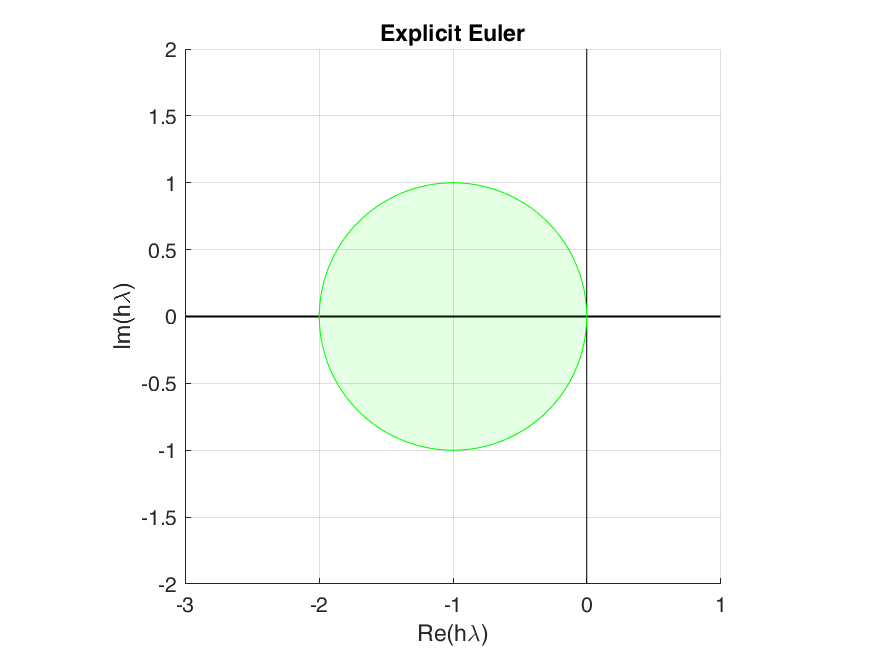
\includegraphics[width=0.48\textwidth]{stability_euler.png}
			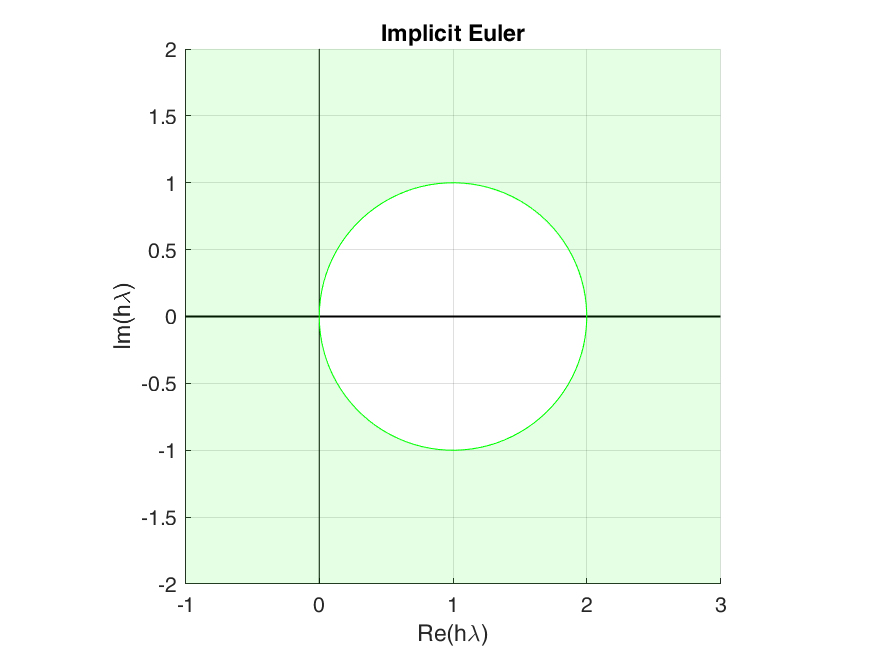
\includegraphics[width=0.48\textwidth]{stability_ieuler.png}
		\caption{Stability region of explicit Euler (left) and stability region of implicit Euler (right)}
		\label{fig:stability_euler}
	\end{figure}
	\begin{figure}[ht]
		\centering
			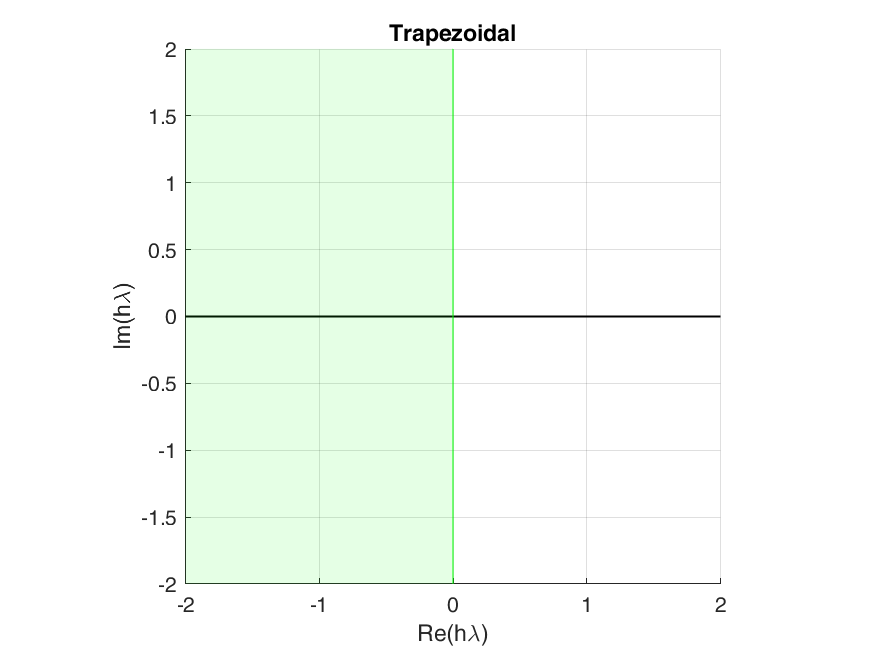
\includegraphics[width=0.48\textwidth]{stability_trapezoidal.png}
			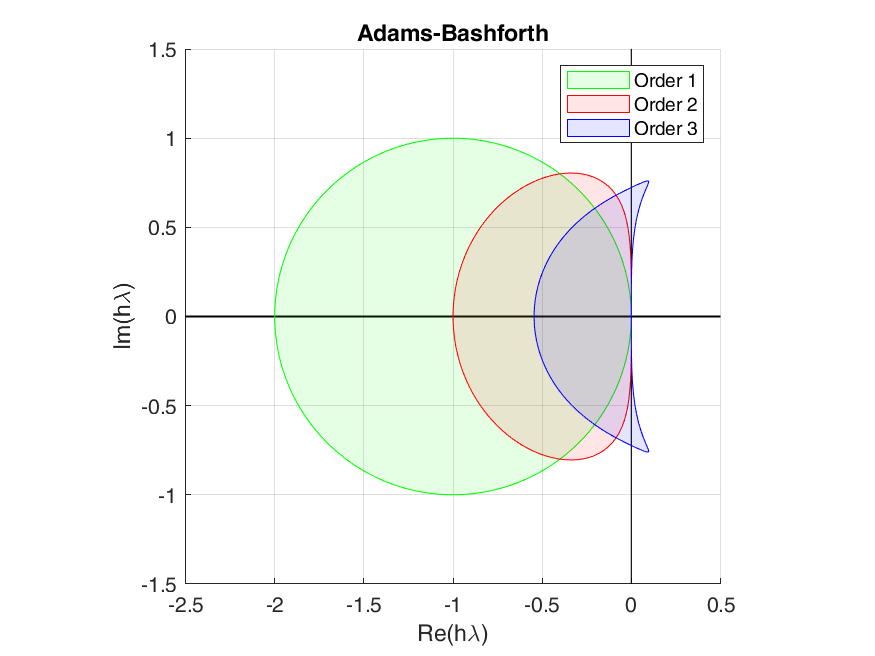
\includegraphics[width=0.48\textwidth]{stability_adams.png}
		\caption{Stability region of trapezoidal method (left) and stability region of Adams-Bashforth (right)}
		\label{fig:stability_euler}
	\end{figure}
	\begin{figure}[ht]
		\centering
			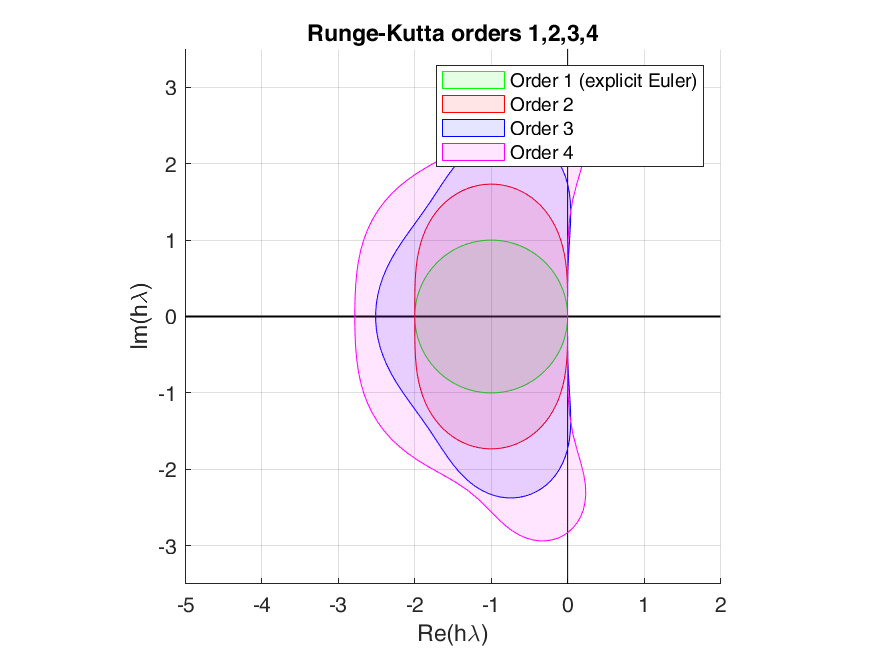
\includegraphics[width=0.48\textwidth]{stability_runge.png}
			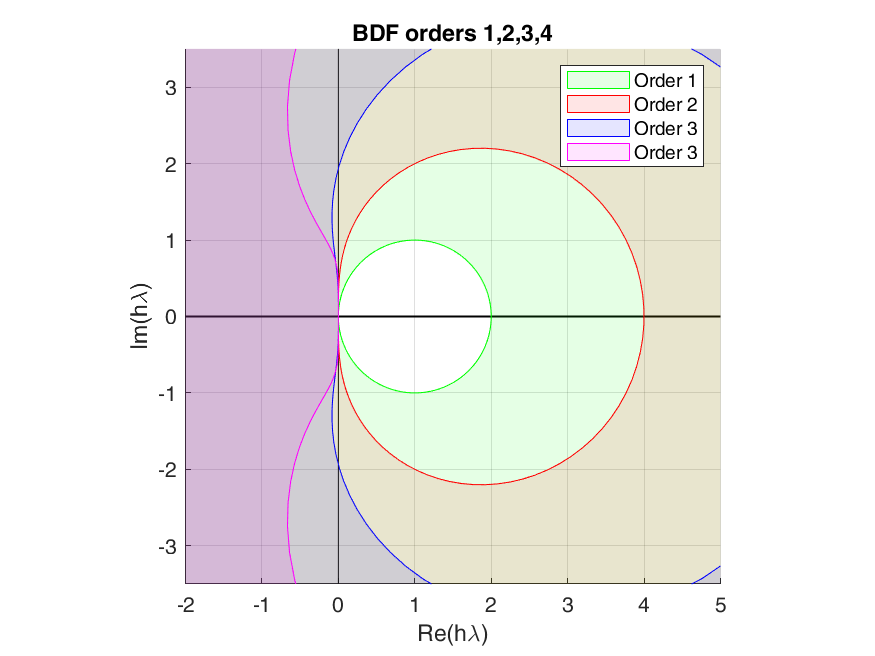
\includegraphics[width=0.48\textwidth]{stability_bdf.png}
		\caption{Stability region of explicit Runge-Kutta (left) and stability region of implicit BDF (right)}
		\label{fig:stability_euler}
	\end{figure}
	
	\item 
	If we can express an integration method, applied to the linearly stiff test equation above, as a product $x_{n+1} = \Phi(h \lambda) x_{n}$, the term $\Phi(h \lambda)$ is called \textbf{stability function}, and one can see that the series converges $\lim_{n \rightarrow \infty} x_{n} = 0$ only for $|\Phi(h \lambda)| < 1$. 
	For the values $h \lambda$ where it holds, the method is called \textbf{linearly stable}. 
	
	\item 
	For a given method, one can plot the region(s) where the linearly stable property holds, as a function of the $h \lambda$ value in the complex plane,
	obtaining areas shown in Fig.\ref{fig:stability_euler}. Those region where the stability function is $|\Phi(h \lambda)| < 1$, is called \textbf{stability region} $\mathcal{R}_A$of the method
	\[
	\mathcal{R}_A = \left\{ h \lambda \, : \,  |\Phi(h \lambda)| < 1 \right\}
	\]
	
	\item
	All methods of practical interest contain the origin $0,0$ of the plane, that is called \textbf{zero-stability}. Note that, for bounded stability regions like circles etc., the larger the $h$ value, or the larger the $\lambda$ value, the farther we go from the origin and the easier we go out of the stability region. This explains why the need of using short $h$ if meeting large stiffness $\lambda$.
	
	\item 
	Methods whose stability region covers at least the entire half plane of negative real values, are called \textit{absolutely stable}, hence the property called \textbf{A-stability}. 
	\[
	\mathrm{A-stability} \; \Leftrightarrow \; \mathcal{R}_A \supseteq \left\{ h \lambda \, : \,  \mathrm{Re} \{h \lambda\} < 0 \right\}
	\]
	Those method converges to zero with the test function regardless of how much stiffness $\lambda$ or how large is $h$. Example: the implicit Euler, the trapezoidal method. Note: not all implicit methods are A-stable, for example BDF of order greater than 2 cover a large portion of the left half plane, but not entirely. 
	
	
	\item 
	Theorem (the \textbf{second Dahlquist barrier}). An A-stable multistep method must be of order $r\leq 2$. 
	\footnote{This means that, despite the efforts, no one would ever invent a method that has absolute stability and integration order greater than 2. If one needs an
	high order because he is concerned with extreme precision, as it happens in celestial mechanics when studying trajectories, probably he better give up with 
	the requirement of absolute stability (luckily enough, in those cases there are no problems of stiff integration).}
	
	\item 
	A more relaxed requirement it the \textbf{A($\alpha$)-stability}, where the stability region must include a cone in the left semiplane, with aperture $2\alpha$:
	\[
	\mathrm{A}\alpha\mathrm{-stability} \; \Leftrightarrow \; \mathcal{R}_A \supseteq \left\{ h \lambda \, : \,  -\alpha < \pi - \mathrm{arg}(h \lambda) < \alpha \right\}
	\]
	
	\item 
	A more stringent requirement is the \textbf{L-stability}, that requires the method to be A-stable plus $\lim_{ h \lambda \rightarrow -\infty} |\Phi(h \lambda)| = 0 $. For instance, the trapezoidal method is A-stable but not L-stable because its $|\Phi(h \lambda)| \rightarrow 1$ when $\lambda \rightarrow -\infty$\footnote{In practical scenarios, this can be seen as the known issue of the trapezoidal method: it dampens decays and harmonics like other implicit methods, but the damping is less and less noticeable for increasing frequencies.}. The implicit Euler is L-stable. 
	
	\item
	From the stronger to the more relaxed property:
	\[
	\mathrm{L-stability}  \Rightarrow \mathrm{A-stability}  \Rightarrow \mathrm{A}\alpha\mathrm{-stability} \rightarrow \mathrm{A}_0\mathrm{-stability}  
	\]
	From a practical perspective, methods that stay on the left of this scale are more and more robust (in the computer science sense, that is, they cope better with unknown and unpredictable systems). For instance, the implicit Euler, although a first order and not so accurate integrator, is often used in VR, videogames and real-time applications because of its L-stability, that make it able to handle sudden stiff situations without exploding into divergence.
	
	\item
	Remember that the stability classes introduced so far are relative to a linearly-stiff test function, but in real scenarios the right hand side can be highly non-linear, therefore it is not guaranteed that even a L-stable method will work all the times. For example, divergence or breakdown of the method could happen for many reasons such as missed convergence in Newton-Raphson iterations, resonance and aliasing with rheonomic terms, finite floating point precision, etc. For instance, if simulating contacts with stiff penalty functions, also L-stable methods could diverge or give unusable results. 
	This said, anyway, L-stable and A-stable method are much less likely to have problems than others.
	
	\item
	Despite the superior stability properties, implicit methods have some drawbacks. First, they introduce some numerical damping, that is more and more visible the larger the $h$ time step. For example, the implicit Euler for DAEs presented in these pages will approach a static analysis for $h\rightarrow \infty$ - look at the formulas. This can be a positive side effect (this artificial numerical damping can be welcome to make the simulation more stable and robust), but if not needed, few implicit methods allow to adjust it, one notable case is the generalized-$\alpha$ method.
	
	\item 
	Another drawback of implicit methods: they require a complex implementation leading to at least 3-4 Newton-Raphson iterations at each time step (hence the need of solving 3-4 linear systems per time step). Explicit integrators on the other hand do not need any linear system to be solved, so they require much less CPU time per each time step. Therefore, implicit integrators pay back if you use large time steps thus making good use of their stability properties. Otherwise, if you must use extremely short time steps anyway, for example for geometric reasons such as when studying high-speed collisions with thin objects, maybe that explicit integrators would be more efficient (as they would be stable anyway with such short time steps).
	
\end{itemize}

\subsection{Exercises}

{
\small

\begin{enumerate}
	
	\item Implement the Runge-Kutta 4th order scheme using Matlab or similar softare tools, and use it to simulate the time integral of a horizontal linear spring-dashpot system attached to a mass, where the parameters are: stiffness $k=1000$Nm, damping  $c=30$Nm/s, mass $m=2$kg. The initial conditions are: $x=0.2$m, $v=0.5$m/s. Test it with increasing time steps $h$ starting from $h=0.002$s and see how precision and stability is affected. 
	
	\item Implement an implicit Euler scheme using Matlab or similar softare tools, and use it to simulate the time integral of a horizontal non-linear spring-dashpot system attached to a mass, where the parameters are: stiffness $k=1000$Nm when $x>0$, $k=100000$Nm when $x\leq0$, damping  $c=30$Nm/s, mass $m=2$kg. The initial conditions are: $x=0.2$m, $v=0.5$m/s. Test it with increasing time steps $h$ starting from $h=0.002$s and see how precision and stability is affected. How does the explicit Euler scheme behaves for the same time steps?
	
	\item A pendulum of length $L=1$m has a disc connected at the lower end, with mass $M=2$kg and inertia $J=0.1$kgm$^2$. The gravitational field is $g=-9.8$ms$^{-2}$ Write the equations of motion as an ODE, with a single generalized coordinate $\theta$ expressing the rotation, and simulate it with an explicit Euler scheme using Matlab or similar tools, from initial conditions $\theta=0.1$rad, $\dot{\theta}=0$rad/s. 
	
	\item For the pendulum of the previous exercise, write the equations of motion as an index-2 DAE, using body coordinates $x,y,\theta$ and unknown reactions in the revolute joint, $\lambda_x, \lambda_y$. How to compute consistent initial values $x_0,y_0,\theta_0, \lambda_{x0},\lambda_{y0}$ from the initial conditions $\theta=0.1$rad, $\dot{\theta}=0$rad/s?
	
	\item For the DAE of the previous exercise, implement a solver using the \textit{implicit Euler for DAE} method presented in this paper, and simulate it. Compare the results to the same pendulum expressed as an ODE and simulated with an explicit Euler scheme. How are the computational times of the DAE solver compared to the ODE solver in this case?
	
	
\end{enumerate}

}


\printbibliography


%%%%%%%%%Bibliography%%%%%%%%
%\bibliographystyle{plain}

%\bibliography{../../../Papers/BibFiles/LaTeXrelated/BibMBS}

%%%%%%%%%%%%%%%%%%%%%%%%%%%%%	


\end{document}



